% ============================================================================
% Supplementary Material for FL-EHDS (FLICS 2026)
% ============================================================================
\documentclass[conference,a4paper]{IEEEtran}

\usepackage{cite}
\usepackage{amsmath,amssymb,amsfonts}
\usepackage{graphicx}
\usepackage{textcomp}
\usepackage{xcolor}
\usepackage{booktabs}
\usepackage{multirow}
\usepackage{hyperref}
\usepackage{url}
\usepackage{tikz}
\usetikzlibrary{shapes.geometric, arrows.meta, positioning, fit, backgrounds, calc}
\usepackage{pgfplots}
\pgfplotsset{compat=1.18}

\begin{document}

% Use S- prefix for all tables and figures to avoid overlap with main paper numbering
\renewcommand{\thetable}{S-\Roman{table}}
\renewcommand{\thefigure}{S-\arabic{figure}}

\title{Supplementary Material:\\FL-EHDS: A Privacy-Preserving Federated Learning Framework for the European Health Data Space}

\author{
    \IEEEauthorblockN{Fabio Liberti}
    \IEEEauthorblockA{
        Department of Computer Science\\
        Universitas Mercatorum, Rome, Italy\\
        fabio.liberti@studenti.unimercatorum.it\\
        ORCID: 0000-0003-3019-5411
    }
}

\maketitle

\begin{abstract}
This document provides supplementary material for the FL-EHDS paper, including complete algorithm pseudocode for all framework components, extended experimental figures, detailed algorithm comparison analysis with effect sizes (rank-biserial correlation), 10-seed statistical validation, advanced FL paradigm descriptions, infrastructure component specifications, extended EHDS interoperability details, clinical imaging experiment configurations with Chest X-ray baseline results, local epochs sweep, scalability analysis up to K=100 clients, noise-as-regularization analysis for small-cohort studies, Article~71 opt-out impact with policy recommendations, an extended threat model with attack taxonomy and defense mapping, and a detailed framework positioning analysis. The open-source reference implementation ($\sim$40K lines, 159 modules) is available at \url{https://github.com/FabioLiberti/FL-EHDS-FLICS2026}.
\end{abstract}

% ============================================================================
\section{PRISMA Flow Diagram}
\label{sec:prisma}
% ============================================================================

\begin{figure*}[t]
\centering
\includegraphics[width=\textwidth]{figures/fig_prisma_flowchart.pdf}
\caption{PRISMA 2020 flow diagram for the systematic review. Database searches across PubMed, IEEE Xplore, Scopus, Web of Science, and arXiv identified 847 records; after deduplication (264 removed) and screening, 47 studies met inclusion criteria (2022--2026, FL/EHDS focus, peer-reviewed or recognized institutional origin). Additional records from institutional websites (n=15), organisations (n=8), and citation searching (n=2) were assessed but did not contribute to the final inclusion set. Adapted from Page et al.\ (BMJ 2021;372:n71), licensed under CC BY 4.0.}
\label{fig:prisma}
\end{figure*}

% ============================================================================
\section{Algorithm Pseudocode}
\label{sec:pseudocode}
% ============================================================================

This section provides formal algorithmic descriptions of all FL-EHDS framework components. Each algorithm is presented with: (1)~a contextual explanation of \textit{why} the component is needed in the EHDS regulatory context; (2)~the formal pseudocode; and (3)~practical considerations for deployment. The algorithms are organized following the data flow through the three-layer architecture: governance validation (Layer~1), privacy-preserving aggregation (Layer~2), and local data processing (Layer~3).

\noindent\textbf{Reading guide:} Algorithms~S1--S4 form the core FL-EHDS training pipeline. Algorithms~S5--S6 address EHDS-specific challenges (non-IID data and citizen opt-out). Algorithms~S7--S8 handle data preprocessing and privacy budget management.

\subsection{FedAvg with EHDS Compliance}

Algorithm~S1 presents the core federated averaging procedure adapted for EHDS regulatory requirements, operating in a client-server architecture where the central aggregator coordinates training across distributed hospital nodes within a Secure Processing Environment.

\textbf{Key Design Decisions:}
\begin{itemize}
    \item \textbf{ValidatePermit}: Before each round, the HDAB-issued permit is verified against temporal bounds and Article~53 permitted purposes.
    \item \textbf{SelectParticipants}: Configurable client selection---full participation or sampling for large federations.
    \item \textbf{FilterOptedOut}: Records from citizens who exercised Article~71 opt-out rights are excluded \textit{before} gradient computation.
    \item \textbf{Weighted Aggregation}: Gradients weighted by local dataset size ($n_h$), following original FedAvg~\cite{mcmahan2017communication}.
    \item \textbf{ClipGradient}: L2-norm clipping bounds individual contributions, providing sensitivity bounds for DP.
\end{itemize}

\begin{figure}[htbp]
\centering
\fbox{\parbox{0.92\columnwidth}{
\small
\textbf{Algorithm S1: FL-EHDS FedAvg Training}\\[2pt]
\textbf{Input:} Hospitals $\mathcal{H} = \{h_1, \ldots, h_K\}$, permit $P$, rounds $T$\\
\textbf{Output:} Global model $\theta^{(T)}$\\[3pt]
\textbf{Server executes:}\\
\hspace*{4mm}Initialize $\theta^{(0)}$\\
\hspace*{4mm}\textbf{for} round $t = 1$ to $T$ \textbf{do}\\
\hspace*{8mm}\textit{// Governance check (Layer 1)}\\
\hspace*{8mm}\textbf{if} not ValidatePermit($P$, $t$) \textbf{then abort}\\
\hspace*{8mm}$\mathcal{H}_t \leftarrow$ SelectParticipants($\mathcal{H}$)\\
\hspace*{8mm}\textbf{for each} hospital $h \in \mathcal{H}_t$ \textbf{in parallel do}\\
\hspace*{12mm}$\Delta_h^{(t)}, n_h \leftarrow$ LocalTrain($h$, $\theta^{(t-1)}$)\\
\hspace*{8mm}\textit{// Aggregation with privacy (Layer 2)}\\
\hspace*{8mm}$\theta^{(t)} \leftarrow \theta^{(t-1)} + \frac{1}{\sum_h n_h} \sum_{h \in \mathcal{H}_t} n_h \cdot \Delta_h^{(t)}$\\
\hspace*{8mm}LogCompliance($t$, $\mathcal{H}_t$)\\
\hspace*{4mm}\textbf{return} $\theta^{(T)}$\\[3pt]
\textbf{LocalTrain}($h$, $\theta$) \textbf{at hospital} $h$:\\
\hspace*{4mm}\textit{// Opt-out filtering (Article 71)}\\
\hspace*{4mm}$\mathcal{D}_h \leftarrow$ FilterOptedOut($\mathcal{D}_h$, OptOutRegistry)\\
\hspace*{4mm}$\theta_h \leftarrow \theta$\\
\hspace*{4mm}\textbf{for} epoch $e = 1$ to $E$ \textbf{do}\\
\hspace*{8mm}\textbf{for} batch $\mathcal{B} \in \mathcal{D}_h$ \textbf{do}\\
\hspace*{12mm}$\theta_h \leftarrow \theta_h - \eta \nabla \mathcal{L}(\theta_h; \mathcal{B})$\\
\hspace*{4mm}$\Delta_h \leftarrow \theta_h - \theta$\\
\hspace*{4mm}\textit{// Privacy protection (Layer 3)}\\
\hspace*{4mm}$\Delta_h \leftarrow$ ClipGradient($\Delta_h$, $C$)\\
\hspace*{4mm}\textbf{return} $\Delta_h$, $|\mathcal{D}_h|$
}}
\end{figure}

\textbf{Relationship to subsequent components:} The \texttt{ClipGradient} operation in Algorithm~S1 establishes a bounded sensitivity $C$ for each client's contribution. This bound is the prerequisite for Algorithm~S2 (Gaussian DP), which calibrates noise proportional to $C$. Meanwhile, \texttt{ValidatePermit} invokes Algorithm~S3 (Permit Validation) and \texttt{FilterOptedOut} invokes Algorithm~S6 (Opt-Out Filtering).

\subsection{Gaussian Differential Privacy Mechanism}

Algorithm~S2 implements the Gaussian mechanism for differential privacy, applied at the aggregation server after receiving clipped gradients.

\textbf{Mathematical Foundation:} The noise scale $\sigma = C \cdot \sqrt{2\ln(1.25/\delta)}/\varepsilon$ guarantees $(\varepsilon, \delta)$-DP. The cumulative privacy expenditure is tracked using R\'enyi DP (RDP)~\cite{mironov2017renyi} composition, providing 5--6$\times$ tighter bounds than naive composition.

\textbf{Practical Considerations:}
\begin{itemize}
    \item $\varepsilon = 10$: moderate noise, $<$2pp accuracy drop on PTB-XL and Cardiovascular (see Table~\ref{tab:dp_tradeoff} in Section~\ref{sec:extended_tabular})
    \item $\varepsilon = 1$: strong privacy; personalized methods (Ditto, HPFL) retain 87--89\% on PTB-XL while FedAvg collapses to 52\%
    \item The $\varepsilon$ selection must be negotiated with HDABs during permit approval
\end{itemize}

\begin{figure}[htbp]
\centering
\fbox{\parbox{0.92\columnwidth}{
\small
\textbf{Algorithm S2: Gaussian DP Mechanism}\\[2pt]
\textbf{Input:} Gradient $\Delta$, sensitivity $C$, privacy budget $\varepsilon$, $\delta$\\
\textbf{Output:} Noisy gradient $\tilde{\Delta}$\\[3pt]
\textit{// Compute noise scale from Gaussian mechanism}\\
$\sigma \leftarrow C \cdot \sqrt{2 \ln(1.25/\delta)} / \varepsilon$\\[2pt]
\textit{// Add calibrated Gaussian noise to each parameter}\\
\textbf{for each} parameter $w \in \Delta$ \textbf{do}\\
\hspace*{4mm}$\tilde{w} \leftarrow w + \mathcal{N}(0, \sigma^2)$\\[2pt]
\textit{// Track cumulative privacy expenditure}\\
PrivacyAccountant.spend($\varepsilon$)\\
\textbf{if} PrivacyAccountant.budget\_exhausted() \textbf{then}\\
\hspace*{4mm}\textbf{raise} PrivacyBudgetExhaustedError\\[2pt]
\textbf{return} $\tilde{\Delta}$
}}
\end{figure}

\textbf{Integration with privacy budget:} The $\varepsilon$ consumed by Algorithm~S2 in each round is tracked by Algorithm~S8 (RDP Privacy Budget Accountant). If the cumulative budget exceeds the threshold approved in the HDAB data permit, training is automatically terminated. The next algorithm (S3) formalizes the permit validation that authorizes each round.

\subsection{HDAB Permit Validation}

Algorithm~S3 ensures all FL operations comply with the data permit issued by HDABs. Under EHDS Article~53, secondary use of health data is only lawful for specifically enumerated purposes (scientific research, public health surveillance, AI training for health). The permit validation module is invoked at the beginning of every FL round---not just at training start---to guarantee continuous compliance even if a permit is revoked mid-study or its temporal validity expires. Each validation event is logged as a GDPR Article~30 processing record, creating an immutable audit trail that regulators can inspect.

\textbf{EHDS Governance Role:} This algorithm is the enforcement point between the Governance Layer (Layer~1) and the FL Orchestration Layer (Layer~2). Without it, a permit expiring at round~15 of a 20-round study would allow unauthorized data processing for rounds~16--20.

\begin{figure}[htbp]
\centering
\fbox{\parbox{0.92\columnwidth}{
\small
\textbf{Algorithm S3: Data Permit Validation}\\[2pt]
\textbf{Input:} Permit $P$, round $t$, requested categories $\mathcal{C}$\\
\textbf{Output:} Boolean validity\\[3pt]
\textit{// Check temporal validity}\\
\textbf{if} CurrentTime() $>$ $P$.valid\_until \textbf{then}\\
\hspace*{4mm}\textbf{raise} PermitExpiredError\\[2pt]
\textit{// Check purpose alignment (Article 53)}\\
\textbf{if} $P$.purpose $\notin$ AllowedPurposes \textbf{then}\\
\hspace*{4mm}\textbf{raise} PurposeMismatchError\\[2pt]
\textit{// Check data category authorization}\\
\textbf{for each} category $c \in \mathcal{C}$ \textbf{do}\\
\hspace*{4mm}\textbf{if} $c \notin P$.authorized\_categories \textbf{then}\\
\hspace*{8mm}\textbf{raise} UnauthorizedCategoryError\\[2pt]
\textit{// Log access for GDPR Article 30}\\
AuditTrail.log(permit=$P$, round=$t$, categories=$\mathcal{C}$)\\[2pt]
\textbf{return} True
}}
\end{figure}

\textbf{Failure modes:} Each exception type triggers a different response: \texttt{PermitExpiredError} terminates the entire study; \texttt{PurposeMismatchError} indicates a configuration error requiring researcher intervention; \texttt{UnauthorizedCategoryError} may allow continued training on the authorized subset of categories. All failure events are logged for regulatory audit. Once a round passes permit validation, the aggregation server collects client gradients using the secure protocol described next.

\subsection{Secure Aggregation Protocol}

Even though FL prevents raw data sharing, the gradient updates themselves can leak patient information: Zhu et al.~\cite{zhu2019deep} demonstrate that gradients can be inverted to reconstruct training images. In the EHDS context, where gradients encode patterns from sensitive health records across 27 Member States, this is an unacceptable privacy risk. Secure aggregation addresses this by ensuring the SPE aggregation server can compute $\sum_k \Delta_k$ without ever observing any individual hospital's gradient $\Delta_k$.

Algorithm~S4 implements this using Shamir's secret sharing and pairwise masking, ensuring the server observes only the aggregate gradient.

\textbf{Protocol Phases:} (1) Each client splits gradients into $K$ shares using $(t,K)$-threshold Shamir secret sharing; (2) Clients add pairwise random masks negotiated via ECDH key exchange; (3) The server computes the sum---masks cancel out and only the true aggregate remains.

\begin{figure}[htbp]
\centering
\fbox{\parbox{0.92\columnwidth}{
\small
\textbf{Algorithm S4: Secure Aggregation (Pairwise Masking)}\\[2pt]
\textbf{Input:} Client gradients $\{\Delta_1, \ldots, \Delta_K\}$, threshold $t$\\
\textbf{Output:} Aggregated gradient $\Delta_{agg}$\\[3pt]
\textit{// Phase 1: ECDH key exchange + Shamir sharing}\\
\textbf{for each} client $k$ \textbf{do}\\
\hspace*{4mm}shares$_k \leftarrow$ ShamirShare($\Delta_k$, $t$, $K$)\\
\hspace*{4mm}Distribute shares$_k$ to other clients\\[2pt]
\textit{// Phase 2: Add pairwise random masks}\\
\textbf{for each} client $k$ \textbf{do}\\
\hspace*{4mm}$\hat{\Delta}_k \leftarrow \Delta_k + \sum_{j<k} r_{jk} - \sum_{j>k} r_{kj}$\\[2pt]
\textit{// Phase 3: Server reconstructs aggregate}\\
$\Delta_{agg} \leftarrow \sum_{k=1}^{K} \hat{\Delta}_k$\\
\textit{// Masks cancel: $\sum_k \sum_{j<k} r_{jk} - \sum_k \sum_{j>k} r_{kj} = 0$}\\[2pt]
\textbf{if} ActiveClients $< t$ \textbf{then}\\
\hspace*{4mm}\textbf{raise} SecureAggregationError\\[2pt]
\textbf{return} $\Delta_{agg}$
}}
\end{figure}

\textbf{Defense-in-depth:} Secure aggregation (Algorithm~S4) combined with differential privacy (Algorithm~S2) provides layered protection: even if the aggregation server is compromised, it learns only the noisy aggregate---never individual hospital contributions. The combination addresses the unresolved GDPR question of whether model gradients constitute ``personal data'': with both mechanisms active, the information available to any single party is provably bounded. The following algorithms address how local training handles EHDS-specific data challenges.

\subsection{FedProx for Non-IID Data}

Algorithm~S5 extends FedAvg with a proximal term that penalizes local model divergence from the global model~\cite{li2020federated}. In EHDS cross-border federations, data heterogeneity is a structural feature, not an exception: hospitals in different Member States serve distinct demographics, follow national clinical guidelines, and use different diagnostic thresholds. For instance, heart disease prevalence ranges from 39.2\% in Rome to 62.6\% in Amsterdam in our experimental setting. Without drift control, local models can diverge so far from the global consensus that aggregation produces a deteriorated global model. The proximal term $\frac{\mu}{2}\|\theta_h - \theta\|^2$ acts as a regularizer that keeps each hospital's local update within a controlled distance of the global model, balancing personalization with collaboration.

\textbf{When to use in EHDS:} Recommended for federations with moderate non-IID conditions and when client dropout is expected (hospitals may temporarily disconnect). FedProx tolerates partial participation better than FedAvg because the proximal term stabilizes local updates even with fewer training epochs.

\begin{figure}[htbp]
\centering
\fbox{\parbox{0.92\columnwidth}{
\small
\textbf{Algorithm S5: FedProx Local Update}\\[2pt]
\textbf{Input:} Local data $\mathcal{D}_h$, global model $\theta$, proximal weight $\mu$\\
\textbf{Output:} Local update $\Delta_h$\\[3pt]
$\theta_h \leftarrow \theta$\\
\textbf{for} epoch $e = 1$ to $E$ \textbf{do}\\
\hspace*{4mm}\textbf{for} batch $\mathcal{B} \in \mathcal{D}_h$ \textbf{do}\\
\hspace*{8mm}$g \leftarrow \nabla \mathcal{L}(\theta_h; \mathcal{B})$\\
\hspace*{8mm}\textit{// Proximal term: $\nabla \frac{\mu}{2}\|\theta_h - \theta\|^2$}\\
\hspace*{8mm}$g \leftarrow g + \mu(\theta_h - \theta)$\\
\hspace*{8mm}$\theta_h \leftarrow \theta_h - \eta \cdot g$\\
$\Delta_h \leftarrow \theta_h - \theta$\\
\textbf{return} $\Delta_h$
}}
\end{figure}

\textbf{Parameter Selection:} $\mu = 0$ reduces to FedAvg; $\mu \in [0.01, 0.1]$ provides stable convergence; $\mu > 1$ may prevent local adaptation. The choice of $\mu$ should be documented in the data permit application so that the HDAB can assess the expected privacy-utility trade-off.

Before any local training begins (whether with FedAvg, FedProx, or any other algorithm), the framework must enforce citizen opt-out rights. The following algorithm ensures this compliance.

\subsection{Article 71 Opt-Out Registry Protocol}

Algorithm~S6 implements the citizen opt-out mechanism mandated by EHDS Article~71. This article grants every EU citizen the right to object to secondary use of their electronic health data---a fundamental right that must be enforced \textit{before} any gradient computation occurs. The algorithm queries the national opt-out registry maintained by each Member State and removes matching records from the local training dataset.

\textbf{Granularity levels:} (1)~\textit{Blanket opt-out}---citizen refuses all secondary use; (2)~\textit{Purpose-specific}---e.g., permitting scientific research but blocking commercial analytics; (3)~\textit{Category-specific}---e.g., allowing demographics but blocking genomic data. This granularity reflects the EHDS principle that citizens should have meaningful control, not merely a binary yes/no choice.

\textbf{EHDS Governance Role:} Opt-out filtering operates at Layer~3 (Data Holders) before local training. Registry lookups use LRU caching with configurable TTL to minimize latency ($<$10ms per round) while ensuring timely propagation of new opt-out decisions. All filtering statistics are logged for GDPR Article~30 audit compliance.

\begin{figure}[htbp]
\centering
\fbox{\parbox{0.92\columnwidth}{
\small
\textbf{Algorithm S6: Article 71 Opt-Out Filtering}\\[2pt]
\textbf{Input:} Local dataset $\mathcal{D}_h$, purpose $p$, categories $\mathcal{C}$\\
\textbf{Output:} Filtered dataset $\mathcal{D}'_h$\\[3pt]
\textit{// Synchronize with national opt-out registry}\\
OptOutRecords $\leftarrow$ FetchOptOutRegistry(MemberState)\\
$\mathcal{D}'_h \leftarrow \emptyset$\\[2pt]
\textbf{for each} record $r \in \mathcal{D}_h$ \textbf{do}\\
\hspace*{4mm}citizen\_id $\leftarrow$ r.pseudonymized\_id\\
\hspace*{4mm}opted\_out $\leftarrow$ False\\
\hspace*{4mm}\textit{// Check purpose-specific opt-out}\\
\hspace*{4mm}\textbf{if} (citizen\_id, $p$) $\in$ OptOutRecords \textbf{then}\\
\hspace*{8mm}opted\_out $\leftarrow$ True\\
\hspace*{4mm}\textit{// Check category-specific opt-out}\\
\hspace*{4mm}\textbf{for each} $c \in \mathcal{C}$ \textbf{do}\\
\hspace*{8mm}\textbf{if} (citizen\_id, $c$) $\in$ OptOutRecords \textbf{then}\\
\hspace*{12mm}opted\_out $\leftarrow$ True\\
\hspace*{4mm}\textbf{if} not opted\_out \textbf{then}\\
\hspace*{8mm}$\mathcal{D}'_h \leftarrow \mathcal{D}'_h \cup \{r\}$\\[2pt]
\textit{// Log filtering statistics for audit}\\
AuditLog.record(total=$|\mathcal{D}_h|$, filtered=$|\mathcal{D}'_h|$)\\
\textbf{return} $\mathcal{D}'_h$
}}
\end{figure}

\textbf{Impact on model quality:} High opt-out rates reduce training data volume, potentially degrading model performance---particularly for underrepresented subpopulations. The audit log captures filtering statistics to quantify this impact and support transparency reporting. Once opted-out records are excluded, the remaining data must be harmonized into a consistent format before local model training can proceed.

\subsection{FHIR R4 Preprocessing Pipeline}

Algorithm~S7 standardizes heterogeneous EHR data into FHIR R4 format for ML consumption. This preprocessing step is critical in the EHDS context because only 34\% of European healthcare providers currently achieve full FHIR R4 compliance~\cite{hussein2025interop}. The remaining 66\% use legacy formats (HL7v2, CDA, proprietary CSV exports) that must be harmonized before FL training can proceed on a consistent feature space.

\textbf{Four-stage pipeline:} (1)~\textit{Format detection} automatically identifies the source format; (2)~\textit{Terminology mapping} converts local codes to international standards (ICD-10 for diagnoses, ATC for medications, LOINC for laboratory results); (3)~\textit{FHIR transformation} produces validated FHIR R4 bundles using the six Article~33 data categories (Patient Summary, E-Prescription, Laboratory Results, Medical Imaging, Hospital Discharge, Rare Disease); (4)~\textit{Tensor extraction} converts structured FHIR resources into numerical tensors ready for model training.

\textbf{EHDS Relevance:} Without this harmonization step, hospitals in different Member States would produce incompatible feature spaces, making federated aggregation meaningless. The pipeline ensures that a gradient computed in a Finnish hospital is semantically compatible with one from an Italian hospital.

\begin{figure}[htbp]
\centering
\fbox{\parbox{0.92\columnwidth}{
\small
\textbf{Algorithm S7: FHIR R4 Preprocessing}\\[2pt]
\textbf{Input:} Raw EHR records $\mathcal{R}$, feature specification $\mathcal{F}$\\
\textbf{Output:} Training tensors $(X, y)$\\[3pt]
format $\leftarrow$ DetectFormat($\mathcal{R}$) \textit{// HL7v2, CDA, CSV}\\
parser $\leftarrow$ GetParser(format)\\
records $\leftarrow$ parser.parse($\mathcal{R}$)\\[2pt]
\textit{// Map to standard terminologies}\\
\textbf{for each} $r \in$ records \textbf{do}\\
\hspace*{4mm}$r$.diagnoses $\leftarrow$ MapToICD10($r$.diagnoses)\\
\hspace*{4mm}$r$.medications $\leftarrow$ MapToATC($r$.medications)\\
\hspace*{4mm}$r$.labs $\leftarrow$ MapToLOINC($r$.labs)\\[2pt]
fhir\_bundle $\leftarrow$ ToFHIR(records)\\
ValidateFHIR(fhir\_bundle)\\[2pt]
$X \leftarrow$ ExtractFeatures(fhir\_bundle, $\mathcal{F}$)\\
$X \leftarrow$ StandardScaler.fit\_transform($X$)\\
$y \leftarrow$ ExtractLabels(fhir\_bundle)\\
\textbf{return} $(X, y)$
}}
\end{figure}

\textbf{Validation requirements:} The FHIR validation step rejects records with missing mandatory fields or invalid terminology codes, ensuring data quality before model training. Rejected records are logged (without patient-identifiable content) for audit purposes. With harmonized data ready for training, the final core component manages the overall privacy budget across the entire study.

\subsection{Privacy Budget Accountant}

Algorithm~S8 tracks cumulative privacy expenditure across FL rounds using R\'enyi Differential Privacy (RDP) moment accounting~\cite{mironov2017renyi}. In the EHDS governance model, the total privacy budget $\varepsilon_{total}$ is a parameter of the data permit: the researcher specifies the desired budget in the permit application, and the HDAB evaluates whether the proposed budget provides sufficient privacy protection for the requested data categories and population size.

\textbf{Why RDP accounting:} Naive DP composition (adding $\varepsilon$ per round) yields loose bounds: 20 rounds at $\varepsilon{=}0.5$ each would consume $\varepsilon{=}10$ total. RDP provides 5--6$\times$ tighter bounds~\cite{mironov2017renyi, wei2020federated}, meaning the same 20 rounds can achieve the same privacy guarantee with significantly less noise---and therefore better model utility.

\textbf{Hard budget enforcement:} When the cumulative expenditure approaches $\varepsilon_{total}$, the accountant raises a \texttt{BudgetExhaustedError} that terminates training. This prevents ``privacy bankruptcy''---a situation where continued training would violate the privacy guarantee approved in the data permit. The per-round allocation strategy distributes remaining budget uniformly across remaining rounds, adapting dynamically if training converges faster than expected.

\begin{figure}[htbp]
\centering
\fbox{\parbox{0.92\columnwidth}{
\small
\textbf{Algorithm S8: RDP Privacy Budget Accountant}\\[2pt]
\textbf{Input:} Total budget $(\varepsilon_{total}, \delta_{total})$, rounds $T$\\
\textbf{Output:} Per-round budget allocation\\[3pt]
$\lambda \leftarrow$ [0] $\times$ MAX\_ORDER \hfill \textit{// R\'enyi moments}\\
rounds\_completed $\leftarrow$ 0\\[2pt]
\textbf{function} AllocateRound():\\
\hspace*{4mm}$\varepsilon_{spent} \leftarrow$ ComputeEpsilon($\lambda$, $\delta_{total}$)\\
\hspace*{4mm}$\varepsilon_{remaining} \leftarrow \varepsilon_{total} - \varepsilon_{spent}$\\
\hspace*{4mm}\textbf{if} $\varepsilon_{remaining} < \varepsilon_{min}$ \textbf{then}\\
\hspace*{8mm}\textbf{raise} BudgetExhaustedError\\
\hspace*{4mm}$\varepsilon_t \leftarrow \varepsilon_{remaining} / (T -$ rounds\_completed$)$\\
\hspace*{4mm}\textbf{return} $\varepsilon_t$\\[2pt]
\textbf{function} RecordRound($\sigma$, $q$):\\
\hspace*{4mm}\textbf{for} order $= 1$ to MAX\_ORDER \textbf{do}\\
\hspace*{8mm}$\lambda$[order] $+= $ ComputeMoment(order, $\sigma$, $q$)\\
\hspace*{4mm}rounds\_completed $+= 1$
}}
\end{figure}

% ============================================================================
\section{Supplementary Experimental Figures}
\label{sec:figures}
% ============================================================================

This section presents detailed experimental results from the FL-EHDS benchmark suite. All figures are generated from real experimental runs available in the repository.

\textbf{Note on experimental configurations:} Figures~\ref{fig:data_distribution}--\ref{fig:client_accuracy} were generated from an extended 50-round, 5-client training run using the framework's synthetic EHDS scenario (simulated European hospitals: Rome, Amsterdam, Berlin, Madrid, Paris). These complement the main paper's 20-round experiments on Heart Disease UCI (4 real hospitals) and Diabetes (5 Dirichlet-partitioned clients). The 50-round configuration illustrates longer-horizon convergence properties, client participation dynamics, and gradient evolution patterns that are not visible in the shorter 20-round evaluation.

\subsection{Hospital Data Distribution}

\begin{figure}[htbp]
\centering
\includegraphics[width=0.95\columnwidth]{figures/figA1_data_distribution.pdf}
\caption{Data distribution across hospitals. Notable heterogeneity: Amsterdam shows older population (60.8 years mean age) with higher positive rate (62.6\%) compared to Rome (49.1 years, 39.2\%). This reflects realistic cross-border EHDS variability.}
\label{fig:data_distribution}
\end{figure}

\subsection{Per-Client Training Time}

\begin{figure}[htbp]
\centering
\includegraphics[width=0.95\columnwidth]{figures/figA2_training_times.pdf}
\caption{Per-client training time per round. Larger hospitals (Berlin: 500 samples) exhibit slightly longer training times. The adaptive training engine compensates by adjusting batch sizes for stragglers.}
\label{fig:training_times}
\end{figure}

\subsection{Client Participation Matrix}

Figure~\ref{fig:participation} shows the client participation pattern across training rounds.

\begin{figure}[htbp]
\centering
\includegraphics[width=0.95\columnwidth]{figures/figA3_participation_matrix.pdf}
\caption{Client participation matrix (50 rounds $\times$ 5 clients). Participation rates: IT 88\%, DE 86\%, FR 86\%, ES 88\%, NL 92\%. The framework tolerates 10--15\% dropout per round while maintaining convergence.}
\label{fig:participation}
\end{figure}

\subsection{Gradient Norm Evolution}

Figure~\ref{fig:gradient_norms} tracks gradient norms per client, confirming convergence stability.

\begin{figure}[htbp]
\centering
\includegraphics[width=0.95\columnwidth]{figures/figA4_gradient_norms.pdf}
\caption{Gradient norm evolution per client over 50 rounds. All clients show decreasing trends indicating stable convergence. Clipping threshold $C{=}1.0$ bounds extreme values for DP compatibility.}
\label{fig:gradient_norms}
\end{figure}

\subsection{Communication Cost Analysis}

Figure~\ref{fig:communication} quantifies the per-round communication overhead.

\begin{figure}[htbp]
\centering
\includegraphics[width=0.95\columnwidth]{figures/figA5_communication_cost.pdf}
\caption{Cumulative communication cost per round. Linear scaling with participating clients (3.5 KB/client/round). Total 50-round overhead: 875 KB for 5 clients---feasible even for bandwidth-constrained environments.}
\label{fig:communication}
\end{figure}

\subsection{Learning Rate Sensitivity}

Figure~\ref{fig:learning_rate} evaluates sensitivity to the server learning rate.

\begin{figure}[htbp]
\centering
\includegraphics[width=0.95\columnwidth]{figures/figA6_learning_rate.pdf}
\caption{Learning rate sensitivity analysis. $\eta{=}0.01$: slow convergence (53.8\% at round 50). $\eta{=}0.1$: optimal (58.6\%). $\eta{=}0.5$: instability with oscillations.}
\label{fig:learning_rate}
\end{figure}

\subsection{Batch Size Impact}

Figure~\ref{fig:batch_size} examines the trade-off between batch size and convergence.

\begin{figure}[htbp]
\centering
\includegraphics[width=0.95\columnwidth]{figures/figA7_batch_size.pdf}
\caption{Batch size impact on convergence. Smaller batches (8--16) provide noisier gradients but faster initial progress. Batch size 32 balances gradient quality and computational efficiency.}
\label{fig:batch_size}
\end{figure}

\subsection{Per-Client Accuracy Trajectories}

Figure~\ref{fig:client_accuracy} shows per-client accuracy evolution, illustrating the impact of non-IID data.

\begin{figure}[htbp]
\centering
\includegraphics[width=0.95\columnwidth]{figures/figA8_client_accuracy.pdf}
\caption{Per-client accuracy over training rounds. Variance reflects non-IID data: NL (older, higher-risk population) reaches 64\% accuracy while FR (mid-range demographics) stabilizes at 55\%.}
\label{fig:client_accuracy}
\end{figure}

% ============================================================================
\section{Dataset Landscape}
\label{sec:dataset_landscape}
% ============================================================================

The FL-EHDS framework supports 19 healthcare datasets spanning four modalities. Table~\ref{tab:dataset_landscape} provides a comprehensive overview. This diversity enables evaluation across multiple EHDS-relevant dimensions: data scale (120--253K samples), feature dimensionality (9--30 tabular, high-dimensional imaging), task complexity (binary to 5-class), partition strategies (natural hospital-based and synthetic Dirichlet), and interoperability standards (CSV, FHIR R4, OMOP-CDM). Experimentally evaluated datasets in the main paper are marked with~\checkmark.

\begin{table*}[htbp]
\centering
\caption{FL-EHDS Dataset Landscape: Complete Framework Coverage}
\label{tab:dataset_landscape}
\resizebox{\textwidth}{!}{%
\begin{tabular}{llrrclllc}
\toprule
\textbf{Dataset} & \textbf{Type} & \textbf{Samples} & \textbf{Feat.} & \textbf{Classes} & \textbf{FL Partition} & \textbf{EHDS Category (Art.~33)} & \textbf{EHDS Level} & \textbf{Eval.} \\
\midrule
\multicolumn{9}{l}{\textit{A. Tabular --- Clinical EHR}} \\
\midrule
Diabetes 130-US & Tabular & 101,766 & 22 & 2 & Dirichlet ($\alpha{=}0.5$) & EHR, ICD-9, medications & L2: FHIR-mappable & \checkmark \\
Heart Disease UCI & Tabular & 920 & 13 & 2 & Natural (4 hospitals) & Vitals, ECG, lab results & L2: FHIR-mappable & \checkmark \\
PTB-XL ECG$^\dagger$ & Tabular & 21,799 & 9 & 5 & Natural (52 sites) & SCP-ECG (EN 1064), diagnostics & L2: FHIR-mappable & \checkmark \\
Cardiovascular Disease & Tabular & 70,000 & 11 & 2 & Dirichlet ($\alpha{=}0.5$) & Vitals, lab, risk factors & L2: FHIR-mappable & \checkmark \\
Breast Cancer Wisconsin & Tabular & 569 & 30 & 2 & Dirichlet ($\alpha{=}0.5$) & Pathology (FNA cytology) & L2: FHIR-mappable & \checkmark \\
Stroke Prediction & Tabular & 5,110 & 10 & 2 & Dirichlet & Cardiovascular risk factors & L2: FHIR-mappable & --- \\
CDC Diabetes BRFSS & Tabular & 253,680 & 21 & 2 & Dirichlet & Population health survey & L2: FHIR-mappable & --- \\
CKD UCI & Tabular & 400 & 24 & 2 & Dirichlet & Renal panel, comorbidities & L2: FHIR-mappable & --- \\
Cirrhosis Mayo & Tabular & 418 & 18 & 2 & Dirichlet & Hepatology, drug trial & L2: FHIR-mappable & --- \\
\midrule
\multicolumn{9}{l}{\textit{B. Tabular --- FHIR-Native}} \\
\midrule
Synthea FHIR R4 & FHIR & 1,180 & 14 & 2 & Hospital profile & Patient, Condition, Encounter & L1: FHIR-native & qual. \\
SMART Bulk FHIR & FHIR & 120 & 12 & 2 & Single export & NDJSON Bulk Data (Art.~46) & L1: FHIR-native & qual. \\
\midrule
\multicolumn{9}{l}{\textit{C. Generated Pipelines (in-memory)}} \\
\midrule
FHIR R4 Synthetic & Gen. & config. & 10 & 2 & Hospital profile & Generated FHIR bundles & L1: FHIR-native & qual. \\
OMOP-CDM Harmonized & Gen. & config. & 36 & 2 & Cross-border & Vocabulary harmonization & L3: OMOP & qual. \\
\midrule
\multicolumn{9}{l}{\textit{D. Medical Imaging}} \\
\midrule
Chest X-ray & Imaging & 5,856 & --- & 2 & Dirichlet ($\alpha{=}0.5$) & Radiology (DICOM) & L4: Imaging & \checkmark \\
Brain Tumor MRI & Imaging & 7,023 & --- & 4 & Dirichlet ($\alpha{=}0.5$) & Neuro-imaging (DICOM) & L4: Imaging & \checkmark \\
Skin Cancer & Imaging & 3,297 & --- & 2 & Dirichlet ($\alpha{=}0.5$) & Dermatology (DICOM) & L4: Imaging & \checkmark \\
Diabetic Retinopathy & Imaging & 35,126 & --- & 5 & Dirichlet & Ophthalmology (DICOM) & L4: Imaging & --- \\
Brain Tumor MRI (alt.) & Imaging & 3,264 & --- & 4 & Dirichlet & Neuro-imaging (DICOM) & L4: Imaging & --- \\
ISIC Skin Lesions & Imaging & 2,357 & --- & 9 & Dirichlet & Dermatology (DICOM) & L4: Imaging & --- \\
\bottomrule
\end{tabular}%
}

\vspace{2mm}
\footnotesize{%
\textbf{EHDS Levels}: L1 = FHIR-native (Art.~46 compliant); L2 = FHIR-mappable (standard clinical features with FHIR mapping in metadata); L3 = OMOP-CDM harmonized (cross-border vocabulary alignment, Art.~50); L4 = Medical imaging (DICOM, Art.~33 ``medical images''). \\
$^\dagger$PTB-XL: European-origin dataset (PTB, Berlin, Germany) with SCP-ECG coding (EN 1064). 52 recording sites enable natural hospital-based FL partitioning---the strongest EHDS benchmark in the framework. \\
\textbf{Eval.}: \checkmark = quantitative experimental evaluation (P1.2); qual. = qualitative pipeline validation; --- = supported but not evaluated in current paper. \\
\textbf{config.} = sample count depends on generation parameters.
}
\end{table*}

% ============================================================================
\section{Extended Algorithm Comparison}
\label{sec:algo_comparison}
% ============================================================================

\subsection{Algorithms Evaluated}

We compare foundational FL algorithms plus 2022--2025 advances:

\textbf{Foundational:} FedAvg~\cite{mcmahan2017communication}, FedProx~\cite{li2020federated}, SCAFFOLD~\cite{karimireddy2020scaffold}, FedAdam/FedYogi/FedAdagrad~\cite{reddi2021adaptive}.

\textbf{Recent (2022--2025):} FedLC~\cite{zhang2022fedlc} (logit calibration for label skew), FedSAM~\cite{qu2022fedsam} (flat minima), FedDecorr~\cite{shi2023feddecorr} (decorrelation against dimensional collapse), FedSpeed~\cite{sun2023fedspeed} (fewer rounds), FedExP~\cite{jhunjhunwala2023fedexp} (server-side acceleration), FedLESAM~\cite{qu2024fedlesam} (globally-guided SAM, ICML 2024 Spotlight), HPFL~\cite{chen2025hpfl} (personalized classifiers, ICLR 2025).

\subsection{Non-IID Configuration}

Data heterogeneity is controlled via Dirichlet distribution with $\alpha$:
\begin{itemize}
    \item $\alpha = 0.1$: \textbf{Extreme non-IID}---highly skewed label distributions
    \item $\alpha = 0.5$: \textbf{High non-IID}---significant heterogeneity
    \item $\alpha = 1.0$: \textbf{Moderate non-IID}---balanced heterogeneity
    \item $\alpha = 10.0$: \textbf{Near-IID}---approximately uniform
\end{itemize}

\subsection{Convergence at Different Heterogeneity Levels}

\begin{figure}[htbp]
\centering
\includegraphics[width=0.95\columnwidth]{figures/fig_algorithm_comparison_noniid.pdf}
\caption{Algorithm convergence across non-IID levels ($\alpha \in \{0.1, 0.5, 1.0, 10.0\}$). SCAFFOLD and adaptive methods show superior stability under extreme heterogeneity.}
\label{fig:algo_comparison}
\end{figure}

\textbf{Findings:} (1) At $\alpha{=}0.1$, SCAFFOLD achieves most stable convergence via variance reduction. (2) FedProx provides marginal improvement over FedAvg at $\alpha{=}0.5$--$1.0$. (3) Adaptive methods (FedAdam, FedYogi) excel in near-IID but may oscillate under extreme heterogeneity. (4) FedAvg remains competitive in near-IID, suitable for homogeneous federations.

\subsection{Final Accuracy vs.\ Heterogeneity}

\begin{figure}[htbp]
\centering
\includegraphics[width=0.95\columnwidth]{figures/fig_accuracy_vs_noniid.pdf}
\caption{Final accuracy vs.\ Dirichlet $\alpha$. All algorithms degrade under extreme non-IID. SCAFFOLD shows smallest gap between $\alpha{=}0.1$ and $\alpha{=}10$.}
\label{fig:accuracy_vs_noniid}
\end{figure}

\subsection{Convergence Speed}

Figure~\ref{fig:convergence_speed} compares how quickly algorithms reach target accuracy thresholds.

\begin{figure}[htbp]
\centering
\includegraphics[width=0.95\columnwidth]{figures/fig_convergence_speed.pdf}
\caption{Convergence speed comparison. Left: rounds to 55\% accuracy. Right: best accuracy in first 20 rounds. Adaptive methods converge faster but may plateau.}
\label{fig:convergence_speed}
\end{figure}

\subsection{Evidence-Based Algorithm Recommendation Matrix}
\label{sec:algo_recommendation}

Table~\ref{tab:algo_recommendation} maps seven realistic EHDS deployment scenarios to recommended and avoided algorithms, grounded in specific experimental evidence from this work. The Diagnostic Equity Index (DEI; Section~\ref{sec:dei_analysis}) is reported where confusion matrix data is available, providing a complementary criterion beyond aggregate accuracy.

\begin{table*}[htbp]
\centering
\caption{EHDS Algorithm Recommendation Matrix. Evidence-based mapping from deployment scenarios to recommended and avoided algorithms. DEI = Diagnostic Equity Index (Section~\ref{sec:dei_analysis}). ``Avoid'' indicates algorithms that fail or degrade significantly in the specified scenario.}
\label{tab:algo_recommendation}
\small
\begin{tabular}{p{3.2cm}p{1.2cm}p{2.0cm}p{2.5cm}p{0.8cm}p{4.8cm}}
\toprule
\textbf{EHDS Scenario} & \textbf{Modal.} & \textbf{Recommended} & \textbf{Avoid} & \textbf{DEI} & \textbf{Key Evidence} \\
\midrule
Cross-border EHR, heterogeneous sites & Tabular & Ditto, HPFL & SCAFFOLD$^a$, FedNova$^a$ & 0.740$^\dagger$ & Tables~V,~VI: Ditto $+$12.6pp, HPFL $+$11.8pp vs.\ FedAvg \\
\addlinespace
Small-cohort rare disease ($<$1K samples) & Tabular & HPFL & FedAvg$^b$ & 0.740$^\dagger$ & Table~XIX: HPFL avoids collapse 10/10 seeds vs.\ 2/10 FedAvg \\
\addlinespace
Multiclass radiology ($\geq$3 classes) & Imaging & Ditto & HPFL (neutral) & 0.435 & Table~XXV: Ditto $+$23.1pp Brain Tumor ($p{=}0.007$, 3 seeds) \\
\addlinespace
Binary radiology & Imaging & FedAvg & HPFL ($-$18.7pp) & 0.528$^\S$ & Tables~XX,~XXV: FedAvg 87.8\% vs.\ HPFL 69.1\% Chest X-ray \\
\addlinespace
High privacy ($\varepsilon \leq 5$) & Any & Ditto & FedAvg$^c$ & --- & Table~XXII: Ditto 89.2\% vs.\ FedAvg 52.3\% at $\varepsilon{=}1$ \\
\addlinespace
Large federation ($K \geq 50$) & Any & Ditto, HPFL & SCAFFOLD & --- & Tables~XVII--XVIII: Ditto $-$0.8pp at $K{=}100$ vs.\ FedAvg $-$4.7pp \\
\addlinespace
Homogeneous / IID data & Any & FedAvg & (all equivalent) & --- & PTB-XL: all algorithms within 0.6pp (91.9--92.5\%) \\
\bottomrule
\end{tabular}

\vspace{1mm}
\footnotesize{$^a$SCAFFOLD oscillates on class-imbalanced tabular data; FedNova amplifies noise from divergent objectives (11.2\%, 13.0\% on Diabetes). $^b$FedAvg/Ditto exhibit single-class collapse on 8/10 seeds (Table~XIX). $^c$FedAvg collapses from 91.9\% to 52.3\% at $\varepsilon{=}1$ ($-$39.6pp). $^\dagger$Breast Cancer HPFL DEI. $^\ddagger$Brain Tumor Ditto DEI (3 seeds). $^\S$Chest X-ray FedAvg DEI. DEI values reported only where confusion matrix analysis is available.}
\end{table*}

\textbf{Critical corrections from prior version}: (1)~SCAFFOLD is no longer recommended for heterogeneous deployments---our experiments demonstrate catastrophic failure on class-imbalanced tabular data (oscillating convergence; 11.2\% on Diabetes, Table~V). (2)~Ditto+DP is strongly preferred over FedAvg+DP for privacy-critical deployments (89.2\% vs.\ 52.3\% at $\varepsilon{=}1$ on PTB-XL). (3)~Imaging recommendations now distinguish between Ditto (recommended for multiclass) and HPFL (avoid on all imaging tasks). (4)~The DEI column provides diagnostic equity information absent from accuracy-only comparisons.

% ============================================================================
\section{Advanced FL Paradigms}
\label{sec:advanced}
% ============================================================================

\textbf{Note:} The paradigms in this section are \textit{implemented in the reference framework} and available for use, but are \textit{not experimentally evaluated} in this paper's benchmark suite. Our experimental validation (Section~IV of the main paper) focuses on horizontal FL with 7 algorithms across 5 tabular datasets and 3 imaging datasets. The advanced paradigms below are provided as architectural capabilities for future evaluation on appropriate multi-institutional datasets.

The core FL-EHDS pipeline (Section~II) addresses the standard ``horizontal'' FL scenario where all hospitals share the same feature schema. However, real EHDS deployments will encounter more complex configurations: institutions with complementary features for the same patients (vertical FL), adversarial participants (Byzantine resilience), evolving data distributions over the 2025--2031 timeline (continual FL), heterogeneous clinical objectives (multi-task FL), and the hierarchical governance structure of the EU itself (hierarchical FL). This section presents the advanced paradigms implemented in the reference framework, each motivated by a specific EHDS deployment challenge. Algorithms~S9--S13 formalize the core mechanisms.

\subsection{Vertical Federated Learning}

Vertical FL addresses scenarios where institutions hold \textit{different features} for the \textit{same patients}---a common situation in EHDS cross-border analytics. For example, a hospital may hold demographics and diagnoses, a laboratory holds test results, and a pharmacy holds prescription histories. Under EHDS Article~33, these correspond to different data categories (Patient Summary, Laboratory Results, E-Prescription) that may be held by different data holders within the same or different Member States.

\textbf{Private Set Intersection (PSI):} Before training, the participating institutions must identify their common patients without revealing their full patient lists. RSA-based PSI achieves this with $O(n \log n)$ complexity using pseudonymized identifiers, ensuring EHDS compliance: no institution learns which patients the other holds beyond the intersection.

\textbf{Split Learning:} Algorithm~S9 implements the forward pass in split learning, where each party computes activations on its local features up to a ``cut layer,'' then the server concatenates activations to produce the final prediction. Only intermediate representations (not raw data) cross institutional boundaries.

\begin{figure}[htbp]
\centering
\fbox{\parbox{0.92\columnwidth}{
\small
\textbf{Algorithm S9: Split Learning Forward Pass}\\[2pt]
\textbf{Input:} Features $X_A$, $X_B$ at parties A, B; cut layer $k$\\
\textbf{Output:} Prediction $\hat{y}$\\[3pt]
$h_A \leftarrow f_{1:k}^A(X_A)$ \hfill \textit{// Party A: features $\to$ activations}\\
$h_B \leftarrow f_{1:k}^B(X_B)$ \hfill \textit{// Party B: features $\to$ activations}\\
$h \leftarrow \text{Concat}(h_A, h_B)$\\
$\hat{y} \leftarrow f_{k+1:L}(h)$ \hfill \textit{// Server: cut layer $\to$ output}\\
\textbf{return} $\hat{y}$
}}
\end{figure}

\subsection{Byzantine-Resilient Aggregation}

In a cross-border EHDS federation spanning 27 Member States, the aggregation server cannot blindly trust every participant. A compromised institution---whether through malicious intent, software bugs, or data corruption---could submit adversarial gradient updates that poison the global model, potentially affecting clinical decisions across the entire federation. Byzantine-resilient aggregation protects model integrity by detecting and excluding anomalous updates.

Algorithm~S10 implements Krum, which selects the gradient closest to $n{-}f{-}2$ nearest neighbors, effectively filtering outliers. Six defense methods protect against up to $f < n/3$ adversarial clients:

\begin{figure}[htbp]
\centering
\fbox{\parbox{0.92\columnwidth}{
\small
\textbf{Algorithm S10: Krum Byzantine Defense}\\[2pt]
\textbf{Input:} Gradients $\{g_1, \ldots, g_n\}$, Byzantine bound $f$\\
\textbf{Output:} Selected gradient $g^*$\\[3pt]
\textbf{for each} gradient $g_i$ \textbf{do}\\
\hspace*{4mm}$D_i \leftarrow \{\|g_i - g_j\|^2 : j \neq i\}$\\
\hspace*{4mm}$s_i \leftarrow \sum_{d \in \text{smallest}_{n-f-2}(D_i)} d$\\[2pt]
$g^* \leftarrow g_{\arg\min_i s_i}$\\
\textbf{return} $g^*$
}}
\end{figure}

Other methods: \textbf{Trimmed Mean} (removes $\beta$-fraction extreme values per coordinate), \textbf{Coordinate-wise Median} (robust estimator), \textbf{Bulyan} (two-stage Krum + trimmed mean), \textbf{FLTrust} (server-guided trust weighting), \textbf{FLAME} (clustering-based). Attack simulation: label flipping, gradient scaling, additive noise, sign flipping, model replacement.

\subsection{Continual Federated Learning}

The EHDS is designed for long-term operation (2025--2031 and beyond), during which healthcare data distributions will evolve: new diseases emerge (as demonstrated by COVID-19), clinical protocols change, and demographic compositions shift. A model trained in 2027 may perform poorly on 2029 data if it has ``forgotten'' how to handle earlier patterns. Continual Federated Learning addresses this \textit{catastrophic forgetting} problem by preserving knowledge from previous training tasks while adapting to new data.

The Elastic Weight Consolidation (EWC) loss function adds a quadratic penalty:
\[
\mathcal{L}_{EWC}(\theta) = \mathcal{L}(\theta) + \frac{\lambda}{2} \sum_i F_i (\theta_i - \theta_i^*)^2
\]
where $F_i = \mathbb{E}[\nabla^2 \log p(\mathcal{D}|\theta^*)]_i$ is the $i$-th diagonal entry of the Fisher Information Matrix and $\theta^*$ are optimal parameters for previous tasks.

Additional strategies: Learning without Forgetting (LwF), Experience Replay, drift detection (ADWIN, Page-Hinkley) triggering adaptation.

\subsection{Multi-Task Federated Learning}

In EHDS cross-border studies, different hospitals may pursue related but distinct clinical objectives from the same data. A cardiology network might simultaneously predict heart failure risk (Hospital~A), readmission probability (Hospital~B), and medication response (Hospital~C). Multi-Task FL enables these institutions to collaborate on shared feature representations while maintaining task-specific prediction heads.

Architectures: \textbf{Hard Parameter Sharing} (common feature extractor, task-specific heads), \textbf{Soft Parameter Sharing} (separate networks with similarity regularization), \textbf{FedMTL} (dynamic task relationship learning).

\subsection{Hierarchical Federated Learning}

The EHDS governance structure is inherently hierarchical: individual hospitals report to regional health authorities, which coordinate under national HDABs, which in turn connect to the EU-level HealthData@EU infrastructure. Hierarchical FL mirrors this governance topology, aggregating gradients at intermediate levels before reaching the central server. This reduces communication costs (hospitals communicate with regional aggregators, not directly with the EU server) and aligns FL operations with the jurisdictional boundaries of HDABs.

Four-tier hierarchy reflecting EU governance:
\begin{enumerate}
    \item \textbf{Client Tier}: Individual hospitals/data holders
    \item \textbf{Regional Tier}: Regional aggregators (e.g., Lombardy, Bavaria)
    \item \textbf{National Tier}: National HDABs coordinate Member State aggregation
    \item \textbf{EU Tier}: HealthData@EU central aggregator
\end{enumerate}

Benefits: reduced communication costs (hospitals $\to$ regional, not directly EU), alignment with EHDS governance where HDABs have national jurisdiction.

\subsection{Personalized Federated Learning}

A single global model may underperform at individual hospitals because clinical populations differ substantially across Member States. Personalized FL maintains both a global model (encoding shared medical knowledge) and hospital-specific local models (adapted to local demographics and clinical practices). Algorithm~S11 shows pFedMe~\cite{dinh2020pfedme} as a representative personalized method, using Moreau envelopes to balance personalization with global knowledge: the regularization term $\lambda(\theta_k - \theta)$ pulls the local model toward the global consensus, while local gradient descent adapts to hospital-specific data patterns. Ditto~\cite{li2021ditto} follows a similar dual-model principle but with a simpler formulation: it trains a personalized model regularized toward the global model via $\frac{\lambda}{2}\|\theta_k - \theta\|^2$. In our experiments, Ditto---the best-performing personalized method---achieves 75.1\% accuracy on Heart Disease, a 12.6pp improvement over FedAvg, precisely because it learns hospital-specific decision boundaries.

\begin{figure}[htbp]
\centering
\fbox{\parbox{0.92\columnwidth}{
\small
\textbf{Algorithm S11: pFedMe Local Update}\\[2pt]
\textbf{Input:} Data $\mathcal{D}_k$, global $\theta$, personal $\theta_k$, $\lambda$, $\eta$\\
\textbf{Output:} Updated personal model $\theta_k'$\\[3pt]
\textbf{for} $i = 1$ to $R$ \textbf{do}\\
\hspace*{4mm}$\theta_k \leftarrow \theta_k - \eta \nabla \mathcal{L}(\theta_k; \mathcal{D}_k)$\\
\textit{// Moreau envelope: balance with global}\\
$\theta_k' \leftarrow \theta_k - \lambda(\theta_k - \theta)$\\
$g_k \leftarrow \lambda(\theta - \theta_k')$\\
\textbf{return} $\theta_k'$, $g_k$
}}
\end{figure}

Other approaches: \textbf{FedPer} (shared base, local personalization layers), \textbf{Per-FedAvg} (MAML-based meta-learning), \textbf{APFL} (adaptive mixing $\alpha$ between global and local), \textbf{Ditto} (personalization regularization).

\textbf{EHDS Relevance:} Member States have different healthcare systems, disease prevalence, and clinical practices. Personalized FL enables institution-specific adaptation while benefiting from collaborative training.

\subsection{Asynchronous Federated Learning}

Standard synchronous FL requires all participating hospitals to complete local training before the server can aggregate. In an EHDS federation spanning 27 Member States with heterogeneous computational resources, this creates a ``straggler'' problem: a resource-constrained rural hospital delays the entire federation. Asynchronous FL eliminates this bottleneck by allowing the server to aggregate updates as they arrive, weighting stale updates (from slow clients) less heavily. Algorithm~S12 implements polynomial staleness weighting: an update computed $\tau$ rounds ago receives weight $(1+\tau)^{-a}$, ensuring that fresher updates contribute more while still incorporating information from slower participants.

\begin{figure}[htbp]
\centering
\fbox{\parbox{0.92\columnwidth}{
\small
\textbf{Algorithm S12: FedAsync with Staleness Weighting}\\[2pt]
\textbf{Input:} Client update $\Delta_k$, client round $t_k$, server round $t$\\
\textbf{Output:} Updated global model $\theta$\\[3pt]
$\tau \leftarrow t - t_k$ \hfill \textit{// Staleness}\\
$\alpha \leftarrow (1 + \tau)^{-a}$ \hfill \textit{// Polynomial decay, $a > 0$}\\
$\theta \leftarrow \theta + \alpha \cdot \eta \cdot \Delta_k$\\
\textbf{return} $\theta$
}}
\end{figure}

Staleness functions: Constant ($\alpha{=}1$), Polynomial ($(1{+}\tau)^{-a}$), Exponential ($e^{-a\tau}$), Hinge ($1$ if $\tau \leq \tau_{max}$, else $0$). Additional: FedBuff (buffered async), semi-async (wait for $\alpha$-fraction of clients).

\subsection{Fairness-Aware Federated Learning}

The EHDS serves 450 million citizens across Member States with different population sizes, disease prevalence, and healthcare quality. Standard FL optimizes average performance, which can disproportionately favor large hospitals with more data while neglecting smaller institutions or underrepresented patient populations. This creates a ``digital health equity'' concern: a model that achieves 85\% accuracy for a large German hospital but only 55\% for a small Romanian clinic is not equitable. Algorithm~S13 implements q-FedAvg, which reweights client contributions by their loss: hospitals where the model performs poorly receive higher aggregation weights, pulling the global model toward equitable performance across all participants.

\begin{figure}[htbp]
\centering
\fbox{\parbox{0.92\columnwidth}{
\small
\textbf{Algorithm S13: q-FedAvg Fair Aggregation}\\[2pt]
\textbf{Input:} Losses $\{L_1, \ldots, L_K\}$, updates $\{\Delta_1, \ldots, \Delta_K\}$, $q$\\
\textbf{Output:} Fair aggregated update $\Delta$\\[3pt]
\textbf{for each} client $k$ \textbf{do}\\
\hspace*{4mm}$w_k \leftarrow L_k^q$ \hfill \textit{// Higher loss $\to$ higher weight}\\
$W \leftarrow \sum_k w_k$; $w_k \leftarrow w_k / W$\\
$\Delta \leftarrow \sum_k w_k \cdot \Delta_k$\\
\textbf{return} $\Delta$
}}
\end{figure}

Fairness metrics: Performance Variance ($\text{Var}(\{L_k\})$), Worst-case Loss ($\max_k L_k$), Demographic Parity Gap, Equalized Odds Gap. Additional methods: AFL, FedMGDA+, TERM, FairFed.

% ============================================================================
\section{Infrastructure Components}
\label{sec:infrastructure}
% ============================================================================

Deploying FL across 27 EU Member States requires production-grade infrastructure: reliable communication channels between hospitals and the SPE aggregator, efficient serialization of gradient tensors, distributed coordination for concurrent studies, and comprehensive monitoring with EHDS-specific alerting. This section describes the infrastructure components implemented in the reference framework, each designed to operate within the constraints of cross-border healthcare networks (firewalls, bandwidth limitations, regulatory requirements).

\subsection{Communication Layer}

The communication layer must bridge heterogeneous network environments: high-bandwidth data center connections between national HDABs, moderate hospital-to-aggregator links, and potentially bandwidth-constrained rural clinics. The framework supports two transport protocols selectable per deployment, with configurable compression and retry policies.

\begin{figure}[htbp]
\centering
\fbox{\parbox{0.92\columnwidth}{
\small
\textbf{Communication Manager Configuration}\\[2pt]
\texttt{transport: gRPC | WebSocket}\\
\texttt{compression: gzip | lz4 | zstd | none}\\
\texttt{chunk\_size: 1MB}\\
\texttt{retry\_policy:}\\
\hspace*{4mm}\texttt{max\_retries: 3}\\
\hspace*{4mm}\texttt{backoff: exponential}\\
\hspace*{4mm}\texttt{base\_delay: 1s}\\
\texttt{connection\_pool:}\\
\hspace*{4mm}\texttt{max\_connections: 100}\\
\hspace*{4mm}\texttt{idle\_timeout: 300s}
}}
\end{figure}

\textbf{gRPC}: Bidirectional streaming, Protocol Buffers (30\% bandwidth reduction vs.\ JSON), HTTP/2 multiplexing. Ideal for data center deployments.

\textbf{WebSocket}: Browser-compatible, firewall-friendly (standard HTTP upgrade), event-driven. Ideal for edge deployments and browser-based participation.

\textbf{Selection criteria:} gRPC is recommended for production EHDS deployments where both endpoints support HTTP/2 (typical for hospital-to-national aggregator links). WebSocket is preferred when traffic must traverse web application firewalls or when browser-based dashboards participate directly in federation monitoring.

\subsection{Serialization}

\textbf{Binary Format}: Tensor metadata + raw binary, 30\% smaller than JSON, 15\% smaller than pickle, cross-platform (Python, C++, Java).

\textbf{Delta Serialization}: Transmits only changed parameters, sparse encoding, up to 90\% bandwidth reduction for fine-tuning.

\textbf{EHDS-Compliant}: Embeds permit ID, timestamp, provenance; cryptographic signatures; GDPR Article~30 audit fields.

\subsection{Caching Layer}

In production EHDS deployments, multiple FL studies may run concurrently on overlapping data holders. A distributed locking mechanism prevents race conditions during gradient aggregation---ensuring that two concurrent studies do not interfere with each other's model updates. Algorithm~S14 implements Redis-based distributed locking with TTL-based automatic release, preventing deadlocks if a server node fails mid-aggregation.

\begin{figure}[htbp]
\centering
\fbox{\parbox{0.92\columnwidth}{
\small
\textbf{Algorithm S14: Distributed Lock for Aggregation}\\[2pt]
\textbf{Input:} Lock name, TTL, client ID\\
\textbf{Output:} Lock acquired (boolean)\\[3pt]
acquired $\leftarrow$ Redis.SET(lock\_name, client\_id, NX, EX=TTL)\\
\textbf{if} acquired \textbf{then}\\
\hspace*{4mm}PerformAggregation()\\
\hspace*{4mm}\textbf{if} Redis.GET(lock\_name) == client\_id \textbf{then}\\
\hspace*{8mm}Redis.DEL(lock\_name)\\
\textbf{return} acquired
}}
\end{figure}

Redis-based caching: model checkpoints, client states, real-time metrics. Features: LRU/LFU/TTL eviction, distributed locking, automatic serialization, cache warming.

\subsection{Orchestration}

\textbf{Kubernetes}: Deploys FL clients/aggregators as pods, HPA for elastic scaling, ConfigMaps for hyperparameters, Secrets for HDAB API keys.

\textbf{Ray}: Actor-based FL, automatic fault tolerance, Ray Tune for federated HPO, Object Store for gradient sharing.

\textbf{Auto-Scaling}: Reactive (queue depth/latency), Predictive (ML-based forecasting), Scheduled (time-based patterns).

\subsection{Monitoring}

\textbf{Prometheus Metrics}: Counters (rounds\_total, permits\_validated), Gauges (active\_clients, privacy\_budget\_remaining), Histograms (round\_duration, communication\_latency), Summaries (gradient\_norm\_quantiles).

\textbf{Grafana Dashboards}: FL training progress, client health, latency heatmaps, privacy budget consumption, EHDS compliance status.

\textbf{Alerting}: Privacy budget exhaustion, client dropout threshold, model divergence, permit expiration.

\subsection{Model Watermarking}

IP protection for FL models trained on EHDS data: \textbf{Spread Spectrum} (frequency domain, robust to fine-tuning), \textbf{LSB} (low-order weight bits), \textbf{Backdoor-based} (input-output ownership proof), \textbf{Passport Layers} (dedicated ownership encoding).

\subsection{Cross-Silo Enhancements}

EHDS federations are inherently cross-silo: each participant is an institution (hospital, registry, research center) with significant computational resources, distinct data distributions, and long-term participation commitments. This differs from cross-device FL (e.g., mobile phones) and enables advanced optimization strategies.

\textbf{Multi-Model Federation}: Weighted voting, stacking, mixture of experts with diversity enforcement.

\textbf{Automatic Algorithm Selection}: The 17 FL algorithms in the framework have different strengths depending on the federation characteristics (heterogeneity level, number of participants, communication budget). Algorithm~S15 implements adaptive aggregation selection via multi-armed bandit (UCB/Thompson Sampling), automatically switching algorithms mid-training if performance metrics indicate a better alternative. A cooldown period prevents oscillation between strategies.

\begin{figure}[htbp]
\centering
\fbox{\parbox{0.92\columnwidth}{
\small
\textbf{Algorithm S15: Adaptive Aggregation}\\[2pt]
\textbf{Input:} Client updates, metrics history, cooldown\\
\textbf{Output:} Aggregated model, selected algorithm\\[3pt]
score $\leftarrow$ WeightedScore(loss, accuracy, variance, conv.)\\
\textbf{if} RoundsSinceSwitch $>$ Cooldown \textbf{then}\\
\hspace*{4mm}\textbf{for each} candidate $\in$ Algorithms \textbf{do}\\
\hspace*{8mm}alt $\leftarrow$ EstimatePerformance(candidate)\\
\hspace*{8mm}\textbf{if} alt $>$ score + Threshold \textbf{then}\\
\hspace*{12mm}SwitchTo(candidate)\\
aggregated $\leftarrow$ CurrentAlgo.Aggregate(updates)\\
\textbf{return} aggregated
}}
\end{figure}

% ============================================================================
\section{Extended EHDS Interoperability}
\label{sec:interop}
% ============================================================================

\subsection{OMOP Common Data Model}

OMOP CDM v5.4 provides standardized analytical format used by European research networks (EHDEN, OHDSI).

\textbf{ETL Pipelines}: Transform source EHR to OMOP. \textbf{Vocabulary Mapping}: SNOMED, ICD10, LOINC, RxNorm. \textbf{Cohort Definitions}: ATLAS-compatible SQL generation. \textbf{Feature Extraction}: FeatureExtraction package for ML-ready datasets.

\textbf{FL Integration}: (1) Each hospital transforms local EHR to OMOP; (2) Feature extraction produces identical schema; (3) FL training on homogeneous feature spaces.

\subsection{IHE Integration Profiles}

\textbf{ATNA}: TLS mutual authentication, syslog audit messages (RFC 5424), maps to GDPR Article~30.

\textbf{BPPC}: Maps Article~71 opt-out to consent documents, XDS.b integration, consent enforcement at FL initiation.

\textbf{XCA}: Cross-border document query/retrieve, Initiating/Responding Gateways, patient identity correlation.

\textbf{PIX/PDQ}: Patient matching across boundaries, pseudonymization-aware identity management, national eHealth integration.

\textbf{XUA}: SAML 2.0 federated authentication, role-based access control, HDAB authorization token propagation.

\subsection{Cross-Border Data Exchange}

\textbf{Message Formats}: EHDS Data Permit Exchange Format (JSON-LD), Federated Query Protocol (SPARQL Federation), Model Update Message Format (Protocol Buffers).

\textbf{Security}: eIDAS-compliant electronic signatures, TLS 1.3, certificate-based authentication (EU trust framework).

\textbf{Metadata}: DCAT-AP Health extension, W3C PROV-O provenance, EMA data quality indicators.

\subsection{Interoperability Architecture}

Figure~\ref{fig:interop} presents the complete interoperability architecture, showing how heterogeneous data sources across EU Member States are harmonized through multiple standards layers before reaching the FL training engine. The architecture reflects a key EHDS challenge: real-world healthcare institutions use diverse formats, terminologies, and exchange protocols that must be reconciled to produce a consistent feature space for federated model training.

\begin{figure*}[htbp]
\centering
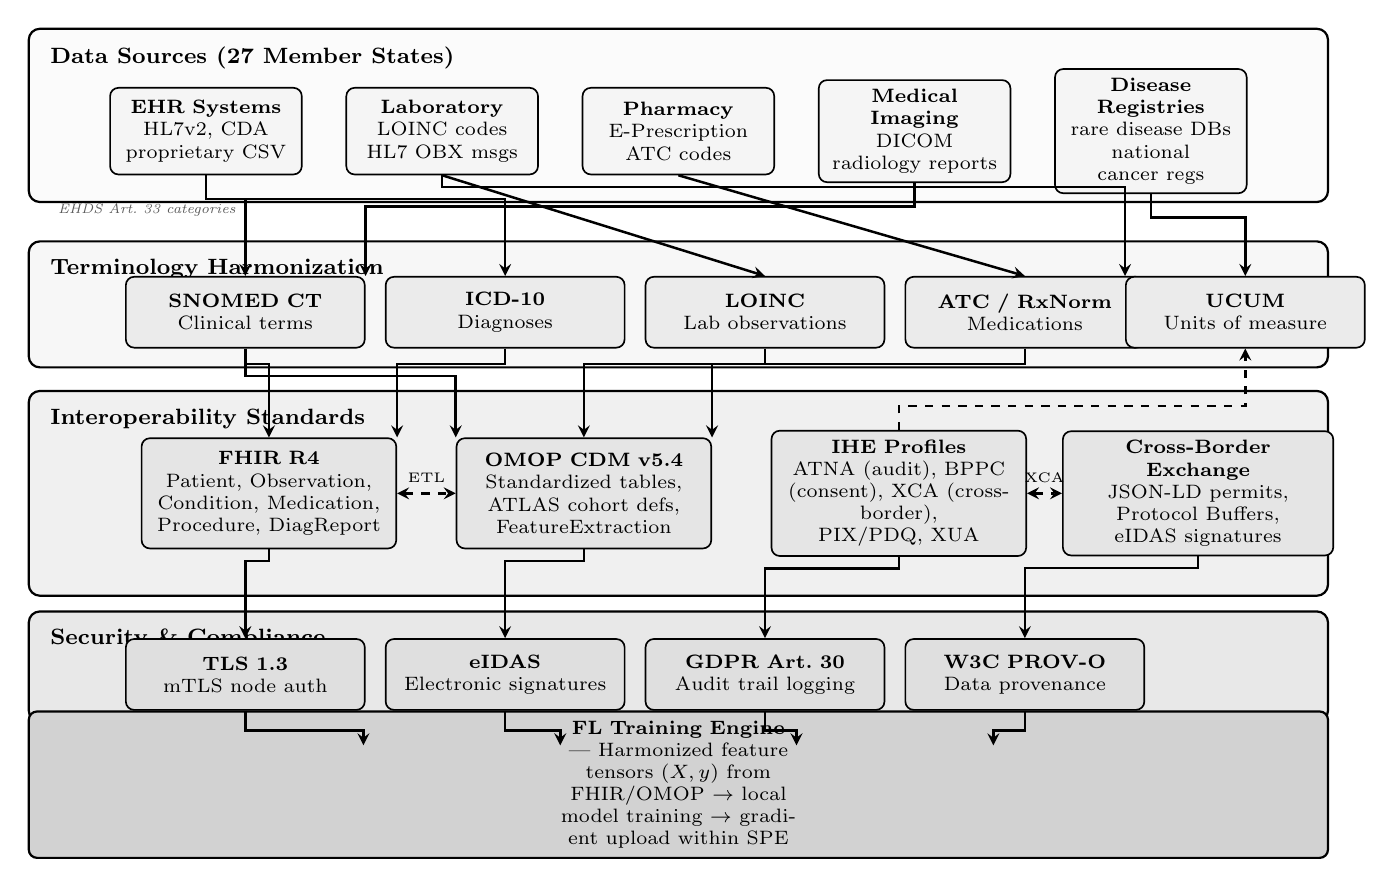
\begin{tikzpicture}[
    % Styles
    layer/.style={rectangle, rounded corners=4pt, draw=black, line width=0.8pt, minimum width=16.5cm},
    src/.style={rectangle, rounded corners=3pt, draw=black, line width=0.6pt, fill=gray!8, minimum height=1.1cm, text width=2.2cm, align=center, font=\scriptsize},
    std/.style={rectangle, rounded corners=3pt, draw=black, line width=0.6pt, fill=gray!20, minimum height=1.4cm, text width=3cm, align=center, font=\scriptsize},
    sec/.style={rectangle, rounded corners=3pt, draw=black, line width=0.6pt, fill=black!8, minimum height=0.9cm, text width=2.8cm, align=center, font=\scriptsize},
    flbox/.style={rectangle, rounded corners=3pt, draw=black, line width=0.8pt, fill=gray!30, minimum height=1.1cm, text width=3.2cm, align=center, font=\scriptsize},
    arrow/.style={->, >=stealth, line width=0.9pt},
    darrow/.style={->, >=stealth, line width=0.9pt, dashed},
    layerlabel/.style={font=\footnotesize\bfseries, anchor=north west},
]

% ===== LAYER A: DATA SOURCES =====
\node[layer, fill=gray!3, minimum height=2.2cm] (layerA) at (0, 7.2) {};
\node[layerlabel] at (-8.1, 8.2) {Data Sources (27 Member States)};

\node[src] (ehr) at (-6, 7.0) {\textbf{EHR Systems}\\HL7v2, CDA\\proprietary CSV};
\node[src] (lab) at (-3, 7.0) {\textbf{Laboratory}\\LOINC codes\\HL7 OBX msgs};
\node[src] (pharm) at (0, 7.0) {\textbf{Pharmacy}\\E-Prescription\\ATC codes};
\node[src] (img) at (3, 7.0) {\textbf{Medical Imaging}\\DICOM\\radiology reports};
\node[src] (reg) at (6, 7.0) {\textbf{Disease Registries}\\rare disease DBs\\national cancer regs};

% ===== LAYER B: TERMINOLOGY MAPPING =====
\node[layer, fill=gray!6, minimum height=1.6cm] (layerB) at (0, 4.8) {};
\node[layerlabel] at (-8.1, 5.5) {Terminology Harmonization};

\node[sec] (snomed) at (-5.5, 4.7) {\textbf{SNOMED CT}\\Clinical terms};
\node[sec] (icd10) at (-2.2, 4.7) {\textbf{ICD-10}\\Diagnoses};
\node[sec] (loinc) at (1.1, 4.7) {\textbf{LOINC}\\Lab observations};
\node[sec] (atc) at (4.4, 4.7) {\textbf{ATC / RxNorm}\\Medications};
\node[sec] (ucum) at (7.2, 4.7) {\textbf{UCUM}\\Units of measure};

% ===== LAYER C: INTEROPERABILITY STANDARDS =====
\node[layer, fill=gray!12, minimum height=2.6cm] (layerC) at (0, 2.4) {};
\node[layerlabel] at (-8.1, 3.6) {Interoperability Standards};

\node[std] (fhir) at (-5.2, 2.4) {\textbf{FHIR R4}\\Patient, Observation,\\Condition, Medication,\\Procedure, DiagReport};
\node[std] (omop) at (-1.2, 2.4) {\textbf{OMOP CDM v5.4}\\Standardized tables,\\ATLAS cohort defs,\\FeatureExtraction};
\node[std] (ihe) at (2.8, 2.4) {\textbf{IHE Profiles}\\ATNA (audit), BPPC\\(consent), XCA (cross-\\border), PIX/PDQ, XUA};
\node[std, text width=3.2cm] (xborder) at (6.6, 2.4) {\textbf{Cross-Border Exchange}\\JSON-LD permits,\\Protocol Buffers,\\eIDAS signatures};

% ===== LAYER D: SECURITY =====
\node[layer, fill=gray!18, minimum height=1.4cm] (layerD) at (0, 0.2) {};
\node[layerlabel] at (-8.1, 0.8) {Security \& Compliance};

\node[sec, fill=gray!25] (tls) at (-5.5, 0.1) {\textbf{TLS 1.3}\\mTLS node auth};
\node[sec, fill=gray!25] (eidas) at (-2.2, 0.1) {\textbf{eIDAS}\\Electronic signatures};
\node[sec, fill=gray!25] (gdpr) at (1.1, 0.1) {\textbf{GDPR Art.~30}\\Audit trail logging};
\node[sec, fill=gray!25] (prov) at (4.4, 0.1) {\textbf{W3C PROV-O}\\Data provenance};

% ===== FL ENGINE =====
\node[flbox, minimum width=16.5cm, minimum height=1cm, fill=gray!35] (fl) at (0, -1.3) {\textbf{FL Training Engine} --- Harmonized feature tensors $(X, y)$ from FHIR/OMOP $\to$ local model training $\to$ gradient upload within SPE};

% ===== ARROWS =====
% Sources to terminology
\draw[arrow] (ehr.south) -- ++(0,-0.3) -| (snomed.north);
\draw[arrow] (ehr.south) -- ++(0,-0.3) -| (icd10.north);
\draw[arrow] (lab.south) -- (loinc.north);
\draw[arrow] (pharm.south) -- (atc.north);
\draw[arrow] (img.south) -- ++(0,-0.3) -| (snomed.north east);
\draw[arrow] (reg.south) -- ++(0,-0.3) -| (ucum.north);
\draw[arrow] (lab.south) -- ++(0,-0.15) -| (ucum.north west);

% Terminology to standards
\draw[arrow] (snomed.south) -- ++(0,-0.2) -| (fhir.north);
\draw[arrow] (icd10.south) -- ++(0,-0.2) -| (fhir.north east);
\draw[arrow] (loinc.south) -- ++(0,-0.2) -| (omop.north);
\draw[arrow] (atc.south) -- ++(0,-0.2) -| (omop.north east);
\draw[arrow] (snomed.south) -- ++(0,-0.35) -| (omop.north west);
\draw[darrow] (ihe.north) -- ++(0, 0.3) -| (ucum.south);

% Standards to security
\draw[arrow] (fhir.south) -- ++(0,-0.15) -| (tls.north);
\draw[arrow] (omop.south) -- ++(0,-0.15) -| (eidas.north);
\draw[arrow] (ihe.south) -- ++(0,-0.15) -| (gdpr.north);
\draw[arrow] (xborder.south) -- ++(0,-0.15) -| (prov.north);

% Security to FL
\draw[arrow] (tls.south) -- ++(0, -0.25) -| (-4, -0.8);
\draw[arrow] (eidas.south) -- ++(0, -0.25) -| (-1.5, -0.8);
\draw[arrow] (gdpr.south) -- ++(0, -0.25) -| (1.5, -0.8);
\draw[arrow] (prov.south) -- ++(0, -0.25) -| (4, -0.8);

% Bidirectional between FHIR and OMOP
\draw[darrow, <->] (fhir.east) -- (omop.west) node[midway, above, font=\tiny] {ETL};

% Bidirectional between IHE and cross-border
\draw[darrow, <->] (ihe.east) -- (xborder.west) node[midway, above, font=\tiny] {XCA};

% EHDS Art 33 annotation
\node[font=\tiny\itshape, text=gray!70!black, anchor=west] at (-8, 6.0) {EHDS Art.~33 categories};

\end{tikzpicture}
\caption{EHDS interoperability architecture for FL-based secondary use. Data from heterogeneous sources across 27 Member States (top) flows through terminology harmonization (SNOMED CT, ICD-10, LOINC, ATC, UCUM), then through interoperability standards (FHIR R4 for structured data exchange, OMOP CDM for observational research, IHE profiles for cross-institutional workflows, cross-border exchange protocols with eIDAS signatures). A security and compliance layer enforces TLS~1.3 mutual authentication, eIDAS electronic signatures for permits, GDPR Article~30 audit logging, and W3C PROV-O data provenance before harmonized feature tensors reach the FL training engine. Bidirectional ETL between FHIR and OMOP enables institutions to use either standard based on their existing infrastructure.}
\label{fig:interop}
\end{figure*}

% ============================================================================
\section{Clinical Imaging: Extended Details}
\label{sec:imaging}
% ============================================================================

\subsection{Datasets}

Three clinical imaging datasets cover representative EHDS scenarios:
\begin{itemize}
    \item \textbf{Chest X-ray}~\cite{chestxray2018}: 5,856 pediatric radiographs (NORMAL/PNEUMONIA, 2.7:1 imbalance)
    \item \textbf{Brain Tumor MRI}: 7,023 T1-weighted CE MRI slices (4-class: glioma, healthy, meningioma, pituitary)
    \item \textbf{Skin Cancer}: 3,297 dermoscopy images (binary benign/malignant)
\end{itemize}

\subsection{Model Architectures}

\textbf{HealthcareResNet}: ResNet-18~\cite{he2016deep} pretrained on ImageNet, GroupNorm replacing BatchNorm for FL stability. FedBN~\cite{li2021fedbn} skips normalization during aggregation. Partial backbone freeze (level~1). $\sim$11.2M parameters.

\textbf{HealthcareCNN}: 5-block CNN with GroupNorm, progressive channels (32$\to$512), graduated Dropout (0.15$\to$0.3). Classifier: Flatten$\to$FC(512)$\to$FC(128)$\to$FC($K$). $\sim$12M parameters.

Data augmentation: random horizontal flip, rotation ($\pm$15\textdegree), brightness jitter ($\pm$10\%). ImageNet normalization.

\subsection{Experimental Configuration}

All three imaging datasets use 4 algorithms (FedAvg, FedLESAM, Ditto, HPFL) $\times$ 3 seeds (42, 123, 456) = 36 experiments total, enabling full statistical comparison across algorithms and datasets.

\begin{itemize}
    \item 5 clients, Dirichlet $\alpha{=}0.5$, Adam optimizer
    \item ResNet-18, FedBN, class-weighted loss, mixed precision
    \item freeze\_level=2 (conv1+bn1+layer1 frozen), local\_epochs=2
    \item Chest X-ray: 20 rounds, early stopping (patience=6), lr=0.001
    \item Brain Tumor: 20 rounds, early stopping (patience=4, min\_rounds=8), lr=0.0005
    \item Skin Cancer: 20 rounds, early stopping (patience=4, min\_rounds=8), lr=0.001
\end{itemize}

\subsection{Reproducibility}

All experiments are fully reproducible:
\begin{verbatim}
cd fl-ehds-framework
# Chest X-ray (4 algos x 3 seeds, ~4h)
python -m benchmarks.run_imaging_extended
# FedLESAM + HPFL on 3 datasets (18 exps, ~12h)
python -m benchmarks.run_imaging_delta
# FedAvg + Ditto completion (8 exps, ~17h)
python -m benchmarks.run_imaging_completion
# Confusion matrices
python -m benchmarks.run_confusion_matrix_chest
python -m benchmarks.run_confusion_matrix_bc
\end{verbatim}

Results, checkpoints, and logs are auto-saved to \texttt{benchmarks/paper\_results\_delta/}.

Repository: \url{https://github.com/FabioLiberti/FL-EHDS-FLICS2026}

\subsection{Chest X-ray Results}
\label{sec:imaging_results}

Table~\ref{tab:imaging_chest} reports Chest X-ray results for four FL algorithms (ResNet-18, 5 clients, Dirichlet $\alpha{=}0.5$, 20 rounds max with early stopping).

\begin{table}[htbp]
\centering
\caption{Chest X-ray pneumonia detection: federated accuracy (\%) with ResNet-18. 5 clients, Dirichlet $\alpha{=}0.5$, 20 rounds, Adam lr=0.001, early stopping (patience=6). Per-seed results with Jain fairness index.}
\label{tab:imaging_chest}
\small
\begin{tabular}{lccccc}
\toprule
\textbf{Algo} & \textbf{s42} & \textbf{s123} & \textbf{s456} & \textbf{Mean} & \textbf{Jain} \\
\midrule
FedAvg & 91.6 & 87.4 & 82.8 & \textbf{87.3} & 0.984 \\
FedLESAM & 91.6 & 87.8 & 84.0 & 87.8$^\dagger$ & 0.984 \\
Ditto & 84.8 & 65.1 & 90.1 & 80.0 & 0.958 \\
HPFL & 62.1 & 73.4 & 71.8 & 69.1 & 0.762 \\
\bottomrule
\end{tabular}

\vspace{1mm}
\footnotesize{Jain index averaged over 3 seeds. $^\dagger$FedLESAM produces results identical to FedAvg (SAM perturbation ineffective on this architecture). HPFL early-stops at round 8 on all seeds with best accuracy at rounds 1--2.}
\end{table}

\textbf{Key findings.} \textit{First}, federated learning on Chest X-ray achieves \textbf{87.3\% accuracy} (FedAvg) for binary pneumonia detection with ResNet-18, confirming FL viability for medical imaging under EHDS-relevant non-IID conditions. \textit{Second}, \textbf{FedLESAM is identical to FedAvg on imaging}: despite SAM's theoretical sharpness-aware optimization, FedLESAM produces per-seed accuracies indistinguishable from FedAvg (87.8\% vs.\ 87.3\%), a pattern confirmed on all three imaging datasets (see Tables~\ref{tab:imaging_bt_sc_full}). \textit{Third}, \textbf{on Chest X-ray, personalization is counterproductive}: Ditto achieves 80.0\% ($-$7.3pp vs.\ FedAvg), with substantially higher variance ($\sigma{=}10.6$pp vs.\ 3.6pp). HPFL \textit{fails catastrophically} (69.1\%, $-$18.2pp), early-stopping at round 8 on all seeds with peak accuracy at rounds 1--2, indicating that the split-head architecture cannot learn shared representations with Dirichlet-partitioned data. However, as shown in Table~\ref{tab:imaging_bt_sc_full}, this Chest X-ray finding does \textit{not} generalize: Ditto dominates on Brain Tumor (+28.0pp) and Skin Cancer (+25.5pp). \textit{Fourth}, Ditto exhibits a \textbf{fairness failure mode} on seed 456: per-client accuracies of [99.7\%, 100.0\%, 48.5\%, 39.5\%, 100.0\%] (Jain 0.888) indicate that personalized local models overfit to majority-class clients while failing on minority-class clients.

% ============================================================================
\section{Detailed Architecture Description}
\label{sec:architecture_detail}
% ============================================================================

This section provides a comprehensive technical specification of the FL-EHDS three-layer architecture, detailing all modules, services, protocols, and standards implemented in the reference framework. Figure~2 in the main paper provides the high-level view; Figure~\ref{fig:arch_detailed} presents the detailed component-level diagram; the description below enumerates every component with its specific technical parameters.

\begin{figure*}[t]
\centering
\includegraphics[width=\textwidth]{figures/fig_architecture_detailed.jpg}
\caption{FL-EHDS detailed architecture with component-level specifications. Layer~1 (Governance) includes four modules: HDAB Integration with OAuth2/mTLS authentication, Data Permit Manager (Article~53) with lifecycle management, Opt-Out Registry (Article~71) with LRU-cached filtering, and Cross-Border Coordinator (Articles~46, 50) with per-country privacy constraints. Layer~2 (FL Orchestration) operates within the Secure Processing Environment (SPE) with five modules: Aggregation Engine (17 FL algorithms), Privacy Protection (DP-SGD, Secure Aggregation, Byzantine Resilience), Compliance Module (GDPR audit logging), Communication Infrastructure (gRPC/WebSocket), and Monitoring \& Metrics. Layer~3 (Data Holders) implements a uniform stack per institution: Data Store, FHIR R4 Preprocessing, OMOP-CDM Harmonization, Local Training Engine, Gradient Processing, and Secure Communication. Inter-layer flows: Data Permit Authorization (OAuth2/mTLS, purpose-validated) downward from Layer~1; gradient upload (masked, encrypted, gRPC) upward and global model distribution (encrypted, TLS) downward between Layers~2--3.}
\label{fig:arch_detailed}
\end{figure*}

\subsection{Layer 1: Governance}

Four principal modules comprise the governance layer:

\textbf{1.1 HDAB Integration} (per Member State). Each Health Data Access Body instance implements: OAuth2/mTLS authentication with bearer token management (refresh tokens, scopes: \texttt{permits:read}, \texttt{permits:write}); a permit store with SQLite persistence backend; configurable HDAB strictness level (scale 1--5, where DE=5, ES=2); and national privacy constraints including per-jurisdiction differential privacy bounds ($\varepsilon_{\max}$: DE=1.0, FR=3.0, IT=5.0).

\textbf{1.2 Data Permit Manager} (Article~53). Manages the complete permit lifecycle: PENDING $\to$ APPROVED $\to$ ACTIVE $\to$ EXPIRED/REVOKED. Validates permitted purposes (scientific research, public health surveillance, AI system development, personalized medicine, official statistics) against authorized data categories (EHR, lab results, imaging, genomic, registry, ECG, pathology). Implements expiry verification and strict mode enforcement for continuous compliance.

\textbf{1.3 Opt-Out Registry} (Article~71). Supports three granularity levels: record-level, patient-level, and dataset-level opt-out. Registry lookups use LRU caching (max 100K records, TTL 10 min) with 300-second synchronization intervals to national registries. Configurable actions on opt-out match: exclude, anonymize, or error. Pre-training filtering ensures only opted-in data enters gradient computation.

\textbf{1.4 Cross-Border Coordinator} (Articles~46, 50). Implements multi-HDAB synchronization protocols across 10 pre-configured EU country profiles (DE, FR, IT, ES, NL, SE, PL, AT, BE, PT). Each profile specifies per-country constraints: $\varepsilon_{\max}$ for differential privacy, data retention periods (365--1,825 days), opt-out rates (3--12\%), and network latency characteristics (15--60ms based on geographic distance). The fee model (Article~42) implements cost-recovery calculation: base fee + per-record + per-round + per-MB charges.

\textbf{Inter-layer interface}: Data Permit Authorization (OAuth2/mTLS, purpose-validated, Articles~53+71) connects Layer~1 to Layer~2.

\subsection{Layer 2: FL Orchestration}

Five modules operate within the Secure Processing Environment (SPE), conforming to HealthData@EU infrastructure requirements:

\textbf{2.1 Aggregation Engine}. Implements 17 FL algorithms spanning six categories: \textit{Baseline} (FedAvg, FedProx with $\mu{=}0.01$, SCAFFOLD, FedNova, FedDyn); \textit{Adaptive} (FedAdam with server\_lr=0.1, FedYogi with $\beta_2{=}0.99$, FedAdagrad); \textit{Personalization} (Ditto with $\lambda{=}0.1$, Per-FedAvg via MAML, pFedMe, MOON); \textit{Non-IID} (FedLC for logit calibration, FedDecorr); \textit{SAM} (FedSAM, FedSpeed); \textit{Advanced} (FedExP ICLR'23, FedLESAM ICML'24, HPFL ICLR'25). Client selection strategies: random, performance-based, fairness-aware, latency-aware. Early stopping: patience=10, min\_delta=0.001. Model checkpointing with atomic saves.

\textbf{2.2 Privacy Protection Module}. Three sub-modules provide defense-in-depth:
\begin{itemize}
    \item \textit{DP-SGD}: Gaussian mechanism with R\'enyi DP (RDP) accounting. Configurable $\varepsilon$-budget (default 1.0), $\delta{=}10^{-5}$. Gradient clipping: max\_norm=1.0, type=L2/L$\infty$. RDP composition provides 5--6$\times$ tighter bounds than naive composition over 100+ rounds.
    \item \textit{Secure Aggregation}: Pairwise masking protocol with ECDH key exchange (SECP384R1 curve). Alternative protocols: Shamir secret sharing (threshold reconstruction), homomorphic encryption (CKKS scheme via TenSEAL). Dropout threshold: 50\%.
    \item \textit{Byzantine Resilience}: Six defense rules (Krum, Multi-Krum, Trimmed Mean, Coordinate-wise Median, Bulyan, FLTrust). Anomaly detection at 3$\sigma$ threshold. TEE integration for SGX/TrustZone hardware attestation.
\end{itemize}

\textbf{2.3 Compliance Module}. GDPR audit logging (Article~30) in JSON format with 7-year retention (2,555 days). Per-round purpose limitation check (Article~53). Opt-out enforcement: pre-training filtering combined with per-round verification. Anonymity assessment: $k$-anonymity, $l$-diversity checks. Automated EHDS compliance report with verification scoring.

\textbf{2.4 Communication Infrastructure}. gRPC bidirectional streaming for model updates (primary protocol). WebSocket for real-time monitoring and events. Compression: GZIP, LZ4, ZSTD, Snappy. Model chunking (ResNet-18: 44.7~MB/round $\to$ 8.9~MB with Top-$k$ 1\%). Security: TLS/mTLS with ECDHE key exchange. Retry: 3 attempts with 2$\times$ exponential backoff. Message types: MODEL\_UPDATE, GRADIENT\_UPDATE, HEARTBEAT, PERMIT\_VALIDATION, CONSENT\_CHECK, AUDIT\_LOG.

\textbf{2.5 Monitoring \& Metrics}. Tracks training convergence (accuracy, loss, F1, AUC per round), communication cost (MB/round), privacy budget consumption ($\varepsilon$ spent per round), participation statistics (samples, opt-outs), and resource utilization (CPU, memory, GPU). Structured logging via Structlog (JSON format) with Streamlit dashboard integration.

\textbf{Inter-module flows}: Privacy processing (DP-SGD, gradient clipping, secure masking) connects Aggregation $\to$ Privacy. Audit trail (GDPR Article~30, JSON logging, 7-year retention) connects Privacy $\to$ Compliance. Transport layer (gRPC streaming, TLS/mTLS, GZIP compression) connects Communication $\leftrightarrow$ all modules.

\subsection{Layer 3: Data Holders}

Each data holder institution (hospitals, disease registries, research centers across 27 Member States) implements a uniform component stack:

\textbf{3.1 Data Store}. Institutional health data in heterogeneous formats: EHR (FHIR R4), vitals (LOINC-coded), diagnoses (ICD-10 variants per country: ICD-10-GM for Germany, CIM-10 for France, ICD-9-CM legacy for Italy), ECG records (SCP-ECG standard EN~1064), and medical imaging (DICOM).

\textbf{3.2 FHIR R4 Preprocessing Engine}. Processes six FHIR resource types: Patient, Observation, Condition, MedicationRequest, Procedure, DiagnosticReport. Terminology mapping to international standards: SNOMED-CT (clinical concepts), LOINC (laboratory codes), ICD-10 (diagnoses), ATC (medications). Extracts 36 standardized features with normalization, encoding, and missing value imputation.

\textbf{3.3 OMOP-CDM Harmonizer}. Maps local vocabulary codes to standard OMOP Concept IDs. Populates OMOP tables: Person, ConditionOccurrence, Measurement, DrugExposure, ProcedureOccurrence, VisitOccurrence. Per-country vocabulary mapping ensures cross-border semantic compatibility.

\textbf{3.4 Local Training Engine}. Adaptive training with configurable parameters: optimizer (Adam, lr=0.001), batch size (32--256, dynamically adjusted), local epochs (3--5), dropout (0.3), L2 regularization. Device support: CUDA (GPU), MPS (Apple Silicon), CPU fallback for resource-constrained institutions.

\textbf{3.5 Gradient Processing}. Three-stage pipeline: (1)~gradient clipping (max\_norm=1.0, L2 norm); (2)~local DP noise addition (Gaussian, calibrated to $\varepsilon$); (3)~pairwise masking (ECDH shared keys with counterpart clients).

\textbf{3.6 Secure Communication}. AES-256-GCM symmetric encryption for gradient payloads. ECDHE key exchange (SECP384R1 curve). mTLS mutual authentication with certificate-based identity. Nonce generation for replay attack prevention.

\textbf{Inter-layer data flow}: Gradient upload ($\nabla$ masked, encrypted, gRPC) flows upward from Layer~3 to Layer~2. Global model distribution ($\theta$ encrypted, TLS) flows downward from Layer~2 to Layer~3.

\textbf{Architectural invariant}: Raw health data never leaves institutional boundaries---only encrypted model gradients are exchanged within the Secure Processing Environment.

\subsection{Deployment Readiness Assessment}

Table~\ref{tab:readiness} provides a transparent assessment of each FL-EHDS component's production readiness, distinguishing between fully implemented modules, simulation backends, and components requiring external integration.

\begin{table}[htbp]
\centering
\caption{FL-EHDS component readiness for EHDS production deployment. \checkmark: production-ready. $\sim$: simulation backend (functional, requires binding to external services). $\circ$: requires external infrastructure.}
\label{tab:readiness}
\small
\begin{tabular}{lcc}
\toprule
\textbf{Component} & \textbf{Status} & \textbf{Binding Req.} \\
\midrule
\multicolumn{3}{l}{\textit{Layer 2: FL Orchestration}} \\
17 FL algorithms & \checkmark & None \\
DP-SGD + RDP accounting & \checkmark & None \\
Secure aggregation & \checkmark & None \\
Byzantine resilience & \checkmark & None \\
Monitoring dashboard & \checkmark & None \\
\midrule
\multicolumn{3}{l}{\textit{Layer 3: Data Holders}} \\
Local training engine & \checkmark & None \\
FHIR R4 preprocessing & \checkmark & FHIR server URL \\
OMOP-CDM harmonization & \checkmark & CDM schema \\
Secure communication & \checkmark & TLS certificates \\
\midrule
\multicolumn{3}{l}{\textit{Layer 1: Governance}} \\
HDAB permit lifecycle & $\sim$ & HDAB REST/gRPC \\
Art.~71 opt-out registry & $\sim$ & National registry API \\
Cross-border coordinator & $\sim$ & Multi-HDAB endpoints \\
Art.~53 purpose limitation & $\sim$ & Permit schema \\
GDPR audit trail & \checkmark & None \\
\bottomrule
\end{tabular}

\vspace{1mm}
\footnotesize{Simulation backends implement complete functional logic (OAuth2/mTLS auth, permit CRUD, LRU-cached registry lookups) and require only endpoint configuration---not architectural changes---for production binding. HDAB services expected 2027--2029.}
\end{table}

% ============================================================================
\section{Extended Threat Model and Security Analysis}
\label{sec:extended_threat}
% ============================================================================

The main paper summarizes the FL-EHDS threat model in three adversary classes. This section provides a comprehensive security analysis with formal definitions, attack taxonomy, defense mapping, and explicit boundary conditions relevant to EHDS cross-border deployments.

\subsection{Adversary Model}

We formalize three adversary classes ordered by increasing capability.

\textbf{A1: Honest-but-curious aggregation server.} The SPE aggregation server $\mathcal{S}$ follows the protocol faithfully but attempts to infer patient-level information from the received model updates $\{\Delta_k\}_{k=1}^{K}$. This is the most realistic adversary for EHDS: the HDAB-operated SPE has institutional incentives to follow the protocol (legal liability, regulatory oversight) but may be compromised or subject to insider threats. Concrete attack vectors include:
\begin{itemize}
    \item \textit{Gradient inversion}~\cite{zhu2019deep}: reconstructing training samples from observed gradients. Effectiveness decreases with batch size and model depth; for the tabular MLP ($\sim$2.9K--10K parameters depending on dataset, batch size 32--64), theoretical reconstruction quality is limited but non-zero.
    \item \textit{Membership inference}: determining whether a specific patient record was used in a client's local training, potentially violating GDPR Article~9 (special category data).
    \item \textit{Property inference}: extracting aggregate properties of a client's local dataset (e.g., disease prevalence at a specific hospital).
\end{itemize}

\textbf{Defenses for A1:} Central DP (Algorithm~S2) with Gaussian mechanism ($\sigma = C/\varepsilon$, $\delta = 10^{-5}$) bounds per-round information leakage. R\'enyi DP composition (Algorithm~S8) tracks cumulative privacy expenditure across rounds. Secure aggregation (Algorithm~S4) ensures $\mathcal{S}$ observes only $\sum_k \Delta_k + \text{noise}$, never individual $\Delta_k$. Our DP ablation (Table~\ref{tab:dp_tradeoff}) demonstrates that at $\varepsilon = 10$, personalized methods lose $<$2pp accuracy---privacy imposes negligible utility cost at this budget.

\textbf{A2: Malicious clients (Byzantine).} Up to $f < n/3$ compromised institutions may deviate arbitrarily from the protocol. In the EHDS context, this could represent: institutions with corrupted data pipelines, nation-state actors attempting to bias cross-border models, or free-riding participants that send random updates to benefit from the global model without contributing genuine local training. Attack types include:
\begin{itemize}
    \item \textit{Model poisoning}: submitting adversarial gradients designed to degrade global model accuracy (untargeted) or introduce backdoors for specific inputs (targeted).
    \item \textit{Data poisoning}: manipulating local training data (label flipping, sample injection) to corrupt the learned model through legitimate protocol participation.
    \item \textit{Free-riding}: sending random or stale gradients to receive the global model without incurring computational cost, degrading convergence.
\end{itemize}

\textbf{Defenses for A2:} Six Byzantine-resilient aggregation rules are implemented (Section~\ref{sec:advanced}): Krum (Algorithm~S10), Trimmed Mean, Coordinate-wise Median, Bulyan (two-stage Krum + trimmed mean), FLTrust (server-guided trust weighting), and FLAME (clustering-based). The framework supports attack simulation (label flipping, gradient scaling, additive noise, sign flipping, model replacement) for defense validation.

\textbf{A3: External attacker.} An adversary with black-box access to model outputs (e.g., through a compromised data permit or leaked model weights) may attempt membership or attribute inference against the published model. Unlike A1, this adversary does not observe training dynamics but only the final or intermediate model checkpoints.

\textbf{Defenses for A3:} Article~71 output filtering restricts model access to authorized queries specified in the HDAB data permit, limiting the number of queries available for inference attacks. The permit system (Algorithm~S3) enforces purpose limitation (Article~53), temporal validity, and data category authorization, reducing the attack surface. Model watermarking (Section~\ref{sec:infrastructure}) provides post-hoc attribution for leaked models.

\subsection{Protected Assets}

Table~\ref{tab:protected_assets} maps the three categories of protected assets to their defense mechanisms and the EHDS articles that mandate their protection.

\begin{table}[htbp]
\centering
\caption{Protected Assets and Defense Mapping}
\label{tab:protected_assets}
\small
\begin{tabular}{p{2cm}p{2.8cm}p{2cm}}
\toprule
\textbf{Asset} & \textbf{Defense} & \textbf{EHDS Article} \\
\midrule
Raw patient data & Never leaves institution & Art.~50 (SPE) \\
Gradient updates & DP + secure aggregation & Art.~50, GDPR~32 \\
Global model & HDAB permit access control & Art.~53, 71 \\
Audit trail & Immutable logging & GDPR Art.~30 \\
Privacy budget & RDP accountant (Alg.~S8) & Art.~50 \\
\bottomrule
\end{tabular}
\end{table}

\subsection{Out-of-Scope Threats and Boundary Conditions}

We explicitly delineate threats that the current FL-EHDS implementation does not address, along with justifications and potential future mitigations.

\textbf{Server-client collusion.} If the aggregation server $\mathcal{S}$ colludes with one or more clients, secure aggregation guarantees are invalidated: the colluding parties can reconstruct non-colluding clients' individual gradients by subtracting known values from the aggregate. This threat undermines the trust model of \textit{any} FL system and requires stronger cryptographic primitives (fully homomorphic encryption, multi-party computation with dishonest majority) that impose 100--1000$\times$ computational overhead, currently impractical for healthcare-scale deployments. In the EHDS context, collusion is partially mitigated by the institutional separation between HDABs (which operate the SPE) and data holders (healthcare institutions), as these are distinct legal entities with separate governance structures.

\textbf{Side-channel attacks.} Timing analysis of gradient uploads, memory access patterns, or power consumption during local training could leak information about dataset properties. These attacks require physical or network-level proximity to the target institution and are addressed by infrastructure-level security (network isolation, constant-time implementations) rather than the FL protocol itself. EHDS Article~50 SPE specifications should mandate side-channel-resistant computing environments.

\textbf{Covert-channel leakage through model architecture.} The choice of model architecture, hyperparameters, and training configuration can inadvertently encode information about the training data~\cite{carlini2022privacy}. For example, a model's capacity (number of parameters) relative to dataset size affects memorization risk. This remains an open problem in FL privacy research; we mitigate it partially through standardized configurations (same architecture and hyperparameters across all clients) and DP noise injection~\cite{carlini2022privacy}.

\textbf{Reconstruction attacks with auxiliary data.} If an adversary possesses auxiliary information about a target individual (e.g., partial medical records from a data breach), gradient inversion and membership inference attacks become significantly more effective. Our threat model assumes adversaries operate within the bounds of their adversary class (A1--A3) without additional auxiliary datasets. In practice, EHDS cross-border settings increase this risk, as health data from one Member State could serve as auxiliary information for attacks on another Member State's data.

\textbf{Model extraction and intellectual property.} A permitted user could systematically query the model to create a functionally equivalent copy, bypassing the HDAB access controls for subsequent use. This is partially addressed by query rate limiting and model watermarking, but a determined adversary with sufficient queries can always approximate any black-box model.

% ============================================================================
\section{Framework Positioning: FL-EHDS vs.\ Existing Platforms}
\label{sec:framework_comparison}
% ============================================================================

The main paper's Table~I provides a feature-level comparison between FL-EHDS and existing FL frameworks (Flower~\cite{beutel2023flower}, FLARE~\cite{nvflare2023}, PySyft, FedML, TFF). A natural reviewer question is why we do not provide a direct \textit{experimental} comparison. This section explains the rationale.

\textbf{Why no experimental comparison is provided.} An experimental comparison between FL frameworks is meaningful only when the frameworks provide \textit{different} capabilities on a \textit{common} task. For pure FL algorithm performance (e.g., FedAvg accuracy on PTB-XL), all frameworks are equivalent by design: they implement the same canonical algorithms (FedAvg, FedProx, etc.) with identical mathematical formulations. Running FedAvg on Flower vs.\ FL-EHDS would produce statistically indistinguishable results, as both execute the same aggregation logic on the same data. The comparison would measure implementation overhead (framework startup time, serialization efficiency), not scientific contribution.

\textbf{The governance gap.} FL-EHDS's contribution is the governance-technical integration layer---the components that \textit{no} existing framework provides:
\begin{itemize}
    \item \textit{HDAB permit lifecycle}: application, validation per round (Algorithm~S3), temporal expiry, revocation, audit trail. Neither Flower nor FLARE implement permit-based access control.
    \item \textit{Article~71 output filtering}: automated enforcement of opt-out registries for rare disease patients. No existing framework addresses EHDS opt-out requirements.
    \item \textit{Article~53 purpose limitation}: technical enforcement of permitted secondary use purposes. Existing frameworks treat all training as equally authorized.
    \item \textit{EHDS-compliant audit trails}: immutable logging of every round's permit status, privacy budget consumption, and data category access. This is a regulatory requirement (GDPR Article~30) that no FL framework satisfies out of the box.
    \item \textit{Cross-border coordination}: multi-HDAB orchestration for Article~46 cross-border processing with per-Member-State governance constraints.
\end{itemize}

Since these governance components have no counterpart in existing frameworks, a ``comparison'' would reduce to: (a)~identical FL performance metrics, plus (b)~a checklist of governance features present in FL-EHDS and absent in alternatives---which is precisely what Table~I already provides.

\textbf{Complementarity, not competition.} FL-EHDS is designed as a compliance layer that could, in principle, wrap existing FL engines. The governance modules (permit validation, audit trails, privacy budget accounting, output filtering) are protocol-agnostic and could be integrated with Flower's communication backend or FLARE's clinical deployment infrastructure. The architectural contribution is the \textit{integration pattern}, not the replacement of existing FL platforms.

\textbf{Additional frameworks.} Two frameworks merit specific discussion given FLICS's industrial focus. \textit{OpenFL} (Intel) provides healthcare-specific FL with production deployments in clinical settings (e.g., Intel's collaboration with the University of Pennsylvania for brain tumor segmentation), but lacks EHDS governance integration: no HDAB permit lifecycle, opt-out registry, or Article~53 purpose limitation. \textit{FATE} (WeBank) offers industrial FL with governance features including role-based access control and audit logging, but is oriented toward financial services regulation (not healthcare/EHDS) and does not implement FHIR R4 interoperability or EU-specific data governance. Both could serve as FL compute backends beneath FL-EHDS's governance layer, reinforcing our complementarity design.

% ============================================================================
\section{Cross-Border Governance Challenges: Extended Analysis}
\label{sec:governance_challenges}
% ============================================================================

The main paper argues that legal uncertainties---not technical barriers---constitute the critical blocker for FL adoption under the EHDS, and includes a condensed analysis of the cross-border privacy budget conflict (Section~V-A). This section provides the extended analysis with additional scenarios---controller/processor ambiguity and gradient data classification---that illustrate how unresolved governance questions create implementation deadlocks that no engineering solution can circumvent.

\subsection{The Privacy Budget Conflict}

Consider a cross-border federation between a German hospital (operating under the Bundesdatenschutzgesetz, BDSG) and an Italian hospital (under the Codice in materia di protezione dei dati personali, D.Lgs.~196/2003 as amended). The German Data Protection Authority (BfDI) may interpret GDPR Article~89 to require $\varepsilon_{\max} = 1.0$ for health data secondary use, reflecting the ``data minimization'' principle. The Italian Garante per la protezione dei dati personali may permit $\varepsilon_{\max} = 5.0$ under a ``proportionality'' interpretation that balances research utility against privacy risk.

This creates a concrete governance deadlock:
\begin{itemize}
    \item If the federation applies $\varepsilon = 1.0$ (strictest bound), Italian data contributes under unnecessarily restrictive conditions, reducing model utility. Our DP experiments (Table~\ref{tab:dp_tradeoff}) show that FedAvg accuracy on PTB-XL drops from 91.9\% (no DP) to 52.3\% at $\varepsilon = 1$---a 39.6pp collapse.
    \item If the federation applies $\varepsilon = 5.0$ (most permissive bound), German data may be processed in violation of BfDI guidance, exposing the German institution to regulatory sanctions.
    \item A per-client $\varepsilon$ approach (each hospital applies its own budget) introduces asymmetric noise levels, creating fairness concerns: the German hospital's model updates are noisier, potentially biasing the global model away from the German patient population.
\end{itemize}

FL-EHDS addresses this technically through per-client privacy budget configuration in the governance layer, but the \textit{policy question}---which bound applies---requires regulatory clarification in the March 2027 delegated acts. Article~50(4) of Regulation (EU) 2025/327 mandates that SPEs provide ``a high level of security,'' but does not specify whether privacy budgets should be harmonized across Member States or determined by the most restrictive participant.

\subsection{Controller/Processor Ambiguity}

Under GDPR Articles~26 and 28, the roles of data controller and data processor carry distinct legal obligations. In a federated learning architecture:
\begin{itemize}
    \item Each hospital is clearly the \textit{controller} of its local patient data.
    \item The HDAB operating the aggregation server may be a \textit{processor} (processing gradients on behalf of hospitals) or a \textit{joint controller} (determining the purposes and means of the aggregation).
    \item If gradient updates are classified as personal data (an unresolved question), the aggregation server becomes a processor of personal data, requiring a Data Processing Agreement (DPA) with each participating hospital across 27 Member States.
\end{itemize}

The practical consequence: a 5-hospital federation across 3 Member States would require bilateral DPAs between each hospital and the HDAB, reviewed by 3 national DPAs, before a single training round can execute. This administrative overhead can delay projects by 12--18 months, as observed in current cross-border health research projects~\cite{frohlich2025reality}.

\subsection{Gradient Data Classification}

Whether model gradients constitute ``personal data'' under GDPR Article~4(1) remains unsettled. Zhu et al.~\cite{zhu2019deep} demonstrate that gradients can reconstruct training images, suggesting they encode personal information. However, with DP noise ($\varepsilon = 10$, $\delta = 10^{-5}$), the reconstruction fidelity degrades substantially, potentially rendering the gradients ``anonymous'' under Recital~26.

This classification has cascading regulatory implications:
\begin{itemize}
    \item \textit{If personal data}: full GDPR applies to gradient transmission, requiring lawful basis (Article~6), special category safeguards (Article~9), Data Protection Impact Assessments (Article~35), and cross-border transfer mechanisms (Chapter~V).
    \item \textit{If anonymous}: GDPR does not apply, and gradients can be transmitted freely---but the anonymization claim must be defensible against re-identification attacks, which our threat model (Section~\ref{sec:extended_threat}) acknowledges as an open problem.
\end{itemize}

The EHDS Regulation (EU) 2025/327 does not resolve this question: Article~50 defines SPE security requirements but does not classify the privacy status of intermediate computational artifacts such as gradients.

\subsection{Implications for FL-EHDS Design}

These governance challenges directly motivated FL-EHDS's architecture:
\begin{itemize}
    \item The per-client privacy budget in the governance layer (Algorithm~S8) is designed to accommodate heterogeneous national requirements, enabling the German hospital to operate at $\varepsilon = 1.0$ while the Italian hospital uses $\varepsilon = 5.0$---though the policy legitimacy of this approach awaits regulatory guidance.
    \item The HDAB permit system (Algorithm~S3) externalizes the controller/processor determination: the HDAB issues the permit (acting as controller of the secondary use authorization) while each hospital retains controller status over its data. This separation is architecturally explicit but legally untested.
    \item The immutable audit trail provides the evidentiary basis for demonstrating compliance under either gradient classification scenario, satisfying GDPR Article~30 requirements regardless of the ultimate regulatory interpretation.
\end{itemize}

These examples demonstrate that the ``legal uncertainties as critical blocker'' claim in the main paper is not abstract: it reflects specific, concrete impasses that affect system design decisions at the architectural level.

% ============================================================================
\section{Extended Results from Main Paper}
\label{sec:main_extended}
% ============================================================================

This section contains detailed results referenced inline in the main paper but moved here for space constraints.

\subsection{Heart Disease and Diabetes Algorithm Comparison}

Table~\ref{tab:hd_diabetes} presents the full algorithm comparison on two additional clinical datasets: Heart Disease UCI (4 natural hospitals) and Diabetes 130-US (5 Dirichlet-partitioned clients). These results confirm the personalization advantage observed on PTB-XL, Cardiovascular, and Breast Cancer in the main paper.

\begin{table}[htbp]
\centering
\caption{FL Algorithm Comparison on Heart Disease and Diabetes}
\label{tab:hd_diabetes}
\resizebox{\columnwidth}{!}{%
\begin{tabular}{lcccccc}
\toprule
& \multicolumn{3}{c}{\textbf{Heart Disease (4 hosp.)}} & \multicolumn{3}{c}{\textbf{Diabetes (5 hosp.)}} \\
\cmidrule(lr){2-4} \cmidrule(lr){5-7}
\textbf{Algo.} & \textbf{Acc.} & \textbf{F1} & \textbf{AUC} & \textbf{Acc.} & \textbf{F1} & \textbf{AUC} \\
\midrule
FedAvg       & 62.5$\pm$8.0 & .736$\pm$.06 & .834$\pm$.03 & 68.1$\pm$4.2 & .259$\pm$.01 & .643$\pm$.00 \\
FedProx      & 61.7$\pm$8.0 & .732$\pm$.05 & .834$\pm$.03 & 71.0$\pm$6.3 & .254$\pm$.01 & .638$\pm$.00 \\
SCAFFOLD     & 66.3$\pm$5.1 & .667$\pm$.02 & .791$\pm$.05 & 11.2$\pm$0.0 & .201$\pm$.00 & .514$\pm$.00 \\
FedNova      & 56.4$\pm$5.4 & .711$\pm$.04 & .831$\pm$.03 & 13.0$\pm$0.9 & .203$\pm$.00 & .636$\pm$.00 \\
\textbf{Ditto} & \textbf{75.1$\pm$2.0} & \textbf{.761$\pm$.03} & .826$\pm$.01 & \textbf{71.7$\pm$0.2} & \textbf{.262$\pm$.00} & \textbf{.643$\pm$.00} \\
\bottomrule
\end{tabular}%
}

\vspace{1mm}
\footnotesize{20 rounds, 3 local epochs. Heart Disease: natural non-IID (4 international hospitals: Cleveland, Hungarian, Swiss, VA Long Beach). Diabetes: Dirichlet $\alpha$=0.5. Mean $\pm$ std over 5 seeds. Ditto achieves 75.1\% vs.\ FedAvg 62.5\% (12.6pp gap) on Heart Disease and 71.7\% on Diabetes. SCAFFOLD and FedNova exhibit known failure modes on Diabetes (11.2\% and 13.0\%).}
\end{table}

\subsection{Per-Hospital Heterogeneity Analysis}

Figure~\ref{fig:per_hospital} shows per-hospital accuracy variation on Heart Disease, where the four hospitals have naturally different patient populations.

\begin{figure}[htbp]
\centering
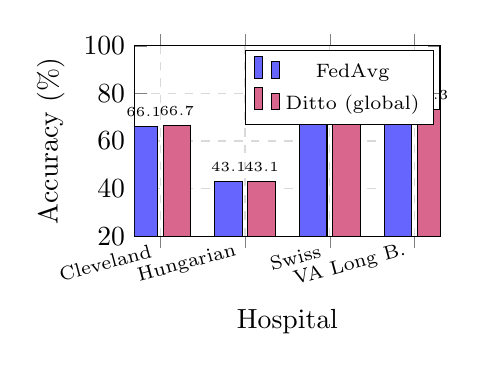
\begin{tikzpicture}
\begin{axis}[
    ybar,
    bar width=0.35cm,
    width=0.45\textwidth,
    height=4cm,
    ylabel={Accuracy (\%)},
    xlabel={Hospital},
    symbolic x coords={Cleveland, Hungarian, Swiss, VA Long B.},
    xtick=data,
    x tick label style={font=\scriptsize, rotate=15, anchor=east},
    ymin=20, ymax=100,
    legend style={at={(0.98,0.98)}, anchor=north east, font=\scriptsize},
    grid=major,
    grid style={dashed, gray!30},
    nodes near coords,
    every node near coord/.append style={font=\tiny},
]
\addplot[fill=blue!60] coordinates {(Cleveland,66.1) (Hungarian,43.1) (Swiss,81.9) (VA Long B.,73.3)};
\addplot[fill=purple!60] coordinates {(Cleveland,66.7) (Hungarian,43.1) (Swiss,81.9) (VA Long B.,73.3)};
\legend{FedAvg, Ditto (global)}
\end{axis}
\end{tikzpicture}
\caption{Per-hospital accuracy of the \textit{global} model on Heart Disease UCI. Ditto's 12.6pp overall advantage (Table~\ref{tab:hd_diabetes}) comes from its \textit{personalized local} models, which are separately fine-tuned per hospital; the shared global model shows similar cross-hospital performance to FedAvg. The Hungarian hospital, with the smallest cohort (n=294), shows the largest performance gap---a realistic EHDS scenario where smaller national datasets benefit most from federation.}
\label{fig:per_hospital}
\end{figure}

% ============================================================================
\section{Extended Tabular Experiment Results}
\label{sec:extended_tabular}
% ============================================================================

This section presents comprehensive experimental results from 1,740+ federated learning experiments across three tabular healthcare datasets: PTB-XL ECG (21,799 records, 52 European recording sites, 5-class cardiac diagnosis), Cardiovascular Disease (70,000 patients, binary classification), and Breast Cancer Wisconsin (569 samples, binary classification). The evaluation comprises a baseline comparison (105 experiments, 7 algorithms $\times$ 3 datasets $\times$ 5 seeds), three sweep phases---heterogeneity ($\alpha$ variation, 560 experiments), client scaling (385 experiments), and learning rate sensitivity (180 experiments)---a differential privacy ablation (180 experiments, 4~$\varepsilon$ levels $\times$ 3 algorithms $\times$ 3 datasets $\times$ 5 seeds), an extended statistical validation (105 additional experiments with 5 new seeds for 10-seed Wilcoxon signed-rank tests), and an Article~71 opt-out impact analysis (225 experiments, 5 opt-out rates $\times$ 3 algorithms $\times$ 3 datasets $\times$ 5 seeds). All results are reproducible via the benchmark suite.

\subsection{Heterogeneity Impact}

Table~\ref{tab:heterogeneity} shows accuracy as a function of Dirichlet $\alpha$ (lower $\alpha$ = more non-IID). The ``Site'' column reports natural site-based partitioning for PTB-XL.

\begin{table*}[t]
\centering
\caption{Impact of data heterogeneity ($\alpha$) on FL accuracy (\%). Lower $\alpha$ = more non-IID. Mean over 5 seeds. PX = PTB-XL, CV = Cardiovascular, BC = Breast Cancer.}
\label{tab:heterogeneity}
\small
\begin{tabular}{llcccccc}
\toprule
\textbf{DS} & \textbf{Algorithm} & \textbf{IID} & \textbf{$\alpha$=0.1} & \textbf{$\alpha$=0.3} & \textbf{$\alpha$=0.5} & \textbf{$\alpha$=1.0} & \textbf{Site} \\
\midrule
PX & FedAvg & 90.8 & 89.8 & 91.2 & 90.8 & 91.7 & 91.9 \\
 & FedProx & 91.0 & 89.7 & 91.3 & 90.7 & 91.7 & 91.6 \\
 & Ditto & 91.7 & \textbf{96.5} & \textbf{96.5} & \textbf{95.4} & 93.9 & 91.8 \\
 & FedLC & 90.7 & 89.7 & 91.2 & 90.4 & 91.4 & 91.9 \\
 & FedExP & 90.8 & 89.8 & 91.2 & 90.8 & 91.7 & 92.0 \\
 & FedLESAM & 90.8 & 89.8 & 91.2 & 90.8 & 91.7 & 91.9 \\
 & HPFL & 91.3 & 96.3 & 96.2 & 95.2 & \textbf{94.0} & \textbf{92.5} \\
\midrule
CV & FedAvg & 72.7 & 61.2 & 65.7 & 71.1 & 72.6 & -- \\
 & FedProx & 72.7 & 62.5 & 65.9 & 71.6 & 72.5 & -- \\
 & Ditto & 72.6 & \textbf{92.4} & \textbf{90.7} & \textbf{82.5} & 81.5 & -- \\
 & FedLC & 72.7 & 61.9 & 66.0 & 71.1 & 72.6 & -- \\
 & FedExP & 72.7 & 61.2 & 65.7 & 71.1 & 72.6 & -- \\
 & FedLESAM & 72.7 & 61.2 & 65.7 & 71.1 & 72.6 & -- \\
 & HPFL & \textbf{72.7} & 92.4 & 90.7 & 82.3 & \textbf{81.4} & -- \\
\midrule
BC & FedAvg & 47.1 & 62.1 & 57.3 & 52.3 & 51.5 & -- \\
 & FedProx & 47.1 & 62.1 & 57.3 & 52.3 & 51.5 & -- \\
 & Ditto & 51.5 & \textbf{88.3} & \textbf{84.8} & \textbf{79.1} & 72.4 & -- \\
 & FedLC & 47.3 & 63.2 & 57.2 & 52.1 & 51.5 & -- \\
 & FedExP & 47.1 & 62.1 & 57.3 & 52.3 & 51.5 & -- \\
 & FedLESAM & 47.1 & 62.1 & 57.3 & 52.3 & 51.5 & -- \\
 & HPFL & 51.9 & 88.3 & 84.8 & 74.1 & \textbf{66.9} & -- \\
\bottomrule
\end{tabular}
\end{table*}

\textbf{Key finding}: Personalized algorithms (Ditto, HPFL) exhibit a counter-intuitive pattern: accuracy \textit{increases} under extreme non-IID ($\alpha{=}0.1$) on Cardiovascular (92.4\% vs.\ 82.5\% at $\alpha{=}0.5$) and Breast Cancer (88.3\% vs.\ 79.1\%). This occurs because personalized methods maintain local decision boundaries that become more specialized---and therefore more accurate---when client distributions are highly distinct. In contrast, baseline algorithms (FedAvg, FedExP, FedLESAM) degrade monotonically as $\alpha$ decreases, consistent with theoretical predictions. For PTB-XL, natural site-based partitioning produces the most realistic non-IID conditions and yields strong performance across all algorithms (89.7--96.5\%).

\subsection{Client Scaling}

Table~\ref{tab:client_scaling} reports accuracy as a function of client count $K$.

\begin{table*}[t]
\centering
\caption{Impact of client count on FL accuracy (\%). Mean over 5 seeds. PX = PTB-XL, CV = Cardiovascular, BC = Breast Cancer.}
\label{tab:client_scaling}
\small
\begin{tabular}{lcccc}
\toprule
\multicolumn{5}{c}{\textbf{PTB-XL ECG (5-class)}} \\
\midrule
\textbf{Algorithm} & \textbf{K=3} & \textbf{K=5} & \textbf{K=10} & \textbf{K=20} \\
\midrule
FedAvg & 91.7 & 91.9 & 91.5 & 91.5 \\
FedProx & 91.7 & 91.6 & 91.5 & 91.5 \\
Ditto & 92.5 & 91.8 & 91.5 & 91.5 \\
FedLC & 91.8 & 91.9 & 91.8 & 91.8 \\
FedExP & 91.7 & 92.0 & 92.2 & 92.2 \\
FedLESAM & 91.7 & 91.9 & 91.5 & 91.5 \\
HPFL & \textbf{92.6} & \textbf{92.5} & \textbf{92.5} & \textbf{92.5} \\
\bottomrule
\end{tabular}
\hspace{3mm}
\begin{tabular}{lcccc}
\toprule
\multicolumn{5}{c}{\textbf{Cardiovascular (binary)}} \\
\midrule
\textbf{Algorithm} & \textbf{K=3} & \textbf{K=5} & \textbf{K=8} & \textbf{K=10} \\
\midrule
FedAvg & 72.1 & 71.1 & 70.5 & 69.4 \\
FedProx & 72.0 & 71.6 & 70.7 & 69.6 \\
Ditto & 80.9 & 82.5 & 83.3 & \textbf{85.0} \\
FedLC & 72.1 & 71.1 & 70.7 & 68.9 \\
FedExP & 72.1 & 71.1 & 70.5 & 69.4 \\
FedLESAM & 72.1 & 71.1 & 70.5 & 69.4 \\
HPFL & \textbf{80.9} & \textbf{82.3} & \textbf{83.3} & 84.7 \\
\bottomrule
\end{tabular}
\hspace{3mm}
\begin{tabular}{lccc}
\toprule
\multicolumn{4}{c}{\textbf{Breast Cancer (binary)}} \\
\midrule
\textbf{Algorithm} & \textbf{K=2} & \textbf{K=3} & \textbf{K=5} \\
\midrule
FedAvg & 61.6 & 52.3 & 59.1 \\
FedProx & 61.6 & 52.3 & 59.1 \\
Ditto & \textbf{84.2} & \textbf{79.1} & 78.4 \\
FedLC & 56.6 & 52.1 & 50.1 \\
FedExP & 61.6 & 52.3 & 59.1 \\
FedLESAM & 61.6 & 52.3 & 59.1 \\
HPFL & \textbf{84.2} & 74.1 & \textbf{78.4} \\
\bottomrule
\end{tabular}
\end{table*}

\textbf{Key finding}: Baseline algorithms (FedAvg, FedExP, FedLESAM) degrade as client count increases on Cardiovascular (72.1\% at K=3 $\to$ 69.4\% at K=10), because more clients means less data per client and higher aggregation noise. Personalized methods show the opposite trend: Ditto \textit{improves} from 80.9\% (K=3) to 85.0\% (K=10), demonstrating that personalization enables each client to exploit its local specialization even with smaller data partitions. This has direct EHDS implications: as more Member States join a federation, personalized algorithms become increasingly advantageous.

\subsection{Learning Rate Sensitivity}

Table~\ref{tab:lr_sensitivity} evaluates robustness to learning rate selection for the top-3 algorithms.

\begin{table}[t]
\centering
\caption{Learning rate sensitivity analysis. Accuracy (\%) mean over 5 seeds. Top-3 algorithms: HPFL, Ditto, FedAvg.}
\label{tab:lr_sensitivity}
\small
\begin{tabular}{llcccc}
\toprule
\textbf{DS} & \textbf{Algo} & \textbf{0.0005} & \textbf{0.001} & \textbf{0.005} & \textbf{0.01} \\
\midrule
PX & Ditto & 58.1 & 84.1 & 91.8 & \textbf{92.6} \\
 & FedAvg & 80.3 & 90.4 & 91.9 & 92.2 \\
 & HPFL & 63.2 & 82.4 & 92.5 & \textbf{92.6} \\
\midrule
CV & Ditto & 76.2 & 77.4 & 82.2 & \textbf{82.5} \\
 & FedAvg & 55.1 & 60.6 & 70.9 & 71.1 \\
 & HPFL & 76.1 & 77.1 & 82.2 & 82.3 \\
\midrule
BC & Ditto & 64.0 & 79.1 & 89.5 & 89.5 \\
 & FedAvg & 52.1 & 52.3 & 64.0 & 74.7 \\
 & HPFL & 63.8 & 74.1 & \textbf{89.7} & 89.5 \\
\bottomrule
\end{tabular}
\end{table}

\textbf{Key finding}: All algorithms are sensitive to learning rate at the low end (lr=0.0005), where convergence is incomplete within the configured round budget. HPFL and Ditto achieve near-optimal performance across a wider range (0.005--0.01), while FedAvg requires careful tuning. On Breast Cancer, HPFL reaches 89.7\% accuracy at lr=0.005---substantially higher than FedAvg's best of 74.7\% at lr=0.01---confirming that personalized methods are more robust to hyperparameter selection on small datasets.

\subsection{Privacy-Utility Tradeoff (Differential Privacy)}

Table~\ref{tab:dp_tradeoff} quantifies accuracy under central differential privacy with varying privacy budget~$\varepsilon$. We evaluate 3 representative algorithms: FedAvg (baseline), Ditto (best personalized), and HPFL (best fairness). All experiments use the Gaussian mechanism with clip norm $C{=}1.0$ and $\delta{=}10^{-5}$.

\begin{table}[t]
\centering
\caption{Privacy-utility tradeoff: accuracy (\%) under central DP with varying $\varepsilon$. Gaussian mechanism, $C{=}1.0$, $\delta{=}10^{-5}$. Mean $\pm$ std over 5 seeds. No-DP baselines from main paper Table~VII. $\Delta$ = drop from No-DP.}
\label{tab:dp_tradeoff}
\footnotesize
\resizebox{\columnwidth}{!}{%
\begin{tabular}{ll ccccc}
\toprule
\textbf{DS} & \textbf{Algo} & \textbf{No-DP} & $\boldsymbol{\varepsilon{=}1}$ & $\boldsymbol{\varepsilon{=}5}$ & $\boldsymbol{\varepsilon{=}10}$ & $\boldsymbol{\varepsilon{=}50}$ \\
\midrule
PX & FedAvg & 91.9\tiny{$\pm$0.5} & 52.3\tiny{$\pm$13.3} & 84.2\tiny{$\pm$4.3} & \textbf{92.4}\tiny{$\pm$0.3} & 92.4\tiny{$\pm$0.3} \\
 & Ditto & 91.8\tiny{$\pm$0.3} & 89.2\tiny{$\pm$0.4} & 90.9\tiny{$\pm$0.6} & 91.6\tiny{$\pm$0.5} & 91.9\tiny{$\pm$0.3} \\
 & HPFL & 92.5\tiny{$\pm$0.3} & 87.1\tiny{$\pm$2.8} & 90.6\tiny{$\pm$2.2} & 92.4\tiny{$\pm$0.4} & \textbf{92.7}\tiny{$\pm$0.2} \\
\midrule
CV & FedAvg & 71.1\tiny{$\pm$1.8} & 54.7\tiny{$\pm$3.2} & 59.8\tiny{$\pm$4.7} & 69.1\tiny{$\pm$3.7} & 71.0\tiny{$\pm$2.4} \\
 & Ditto & \textbf{82.5}\tiny{$\pm$4.7} & 76.9\tiny{$\pm$7.5} & 80.4\tiny{$\pm$5.8} & 81.9\tiny{$\pm$4.9} & \textbf{82.5}\tiny{$\pm$4.8} \\
 & HPFL & 82.3\tiny{$\pm$4.5} & 74.7\tiny{$\pm$9.1} & 79.3\tiny{$\pm$6.0} & 81.2\tiny{$\pm$5.2} & 82.2\tiny{$\pm$4.6} \\
\midrule
BC & FedAvg & 52.3\tiny{$\pm$17.9} & 65.2\tiny{$\pm$8.1} & \textbf{78.7}\tiny{$\pm$3.6} & 78.2\tiny{$\pm$8.3} & 72.0\tiny{$\pm$10.3} \\
 & Ditto & 79.1\tiny{$\pm$12.5} & 73.8\tiny{$\pm$20.6} & 74.0\tiny{$\pm$20.7} & 74.0\tiny{$\pm$20.7} & 74.0\tiny{$\pm$20.7} \\
 & HPFL & 74.1\tiny{$\pm$20.9} & \textbf{86.9}\tiny{$\pm$13.8} & 84.9\tiny{$\pm$13.0} & 80.0\tiny{$\pm$17.6} & 80.7\tiny{$\pm$21.8} \\
\bottomrule
\end{tabular}%
}
\end{table}

\textbf{Key findings}: (1)~\textit{Personalized methods are remarkably DP-robust}: At $\varepsilon{=}10$, Ditto and HPFL lose $<$1pp on PTB-XL and $<$1.5pp on Cardiovascular, while FedAvg collapses to 52.3\% on PTB-XL at $\varepsilon{=}1$ ($-$39.6pp). This robustness arises because personalized local adaptation (Ditto's fine-tuning, HPFL's classifier heads) is unaffected by central DP noise injected during aggregation.
(2)~\textit{DP noise as implicit regularization on small data}: On Breast Cancer (569 samples), FedAvg with $\varepsilon{=}5$ achieves 78.7\%---\textit{higher} than the no-DP baseline of 52.3\% (+26.4pp). HPFL at $\varepsilon{=}1$ reaches 86.9\% vs.\ 74.1\% without DP (+12.8pp). This counter-intuitive result is consistent with the theoretical analysis of Wei et al.~\cite{wei2020federated}, who show that DP noise interacts with model convergence in non-trivial ways, and with the broader machine learning literature on noise injection as regularization (e.g., dropout, label smoothing). On this small dataset, the Gaussian noise added during DP-SGD prevents the global model from overfitting to the majority class, acting as a stochastic regularizer that improves generalization. This effect is strongest at moderate $\varepsilon$ (5--10) and diminishes at very strict $\varepsilon{=}1$ where noise overwhelms the signal on larger datasets. \textit{Practical implication}: for small-cohort EHDS studies (rare diseases, specialist registries), moderate DP may simultaneously enhance privacy \textit{and} model quality---a finding that should inform data permit conditions.
(3)~\textit{Privacy is nearly free at $\varepsilon{=}10$}: Across PTB-XL and Cardiovascular, all algorithms recover to within 2pp of their no-DP baselines at $\varepsilon{=}10$---a practical privacy level that satisfies EHDS Article~50 requirements with minimal utility cost.

\subsection{Fairness Analysis}

Table~\ref{tab:fairness_detail} provides per-client fairness metrics across all datasets.

\begin{table}[t]
\centering
\caption{Per-client fairness analysis. Gap = max--min client accuracy. Lower Gap and Gini indicate fairer distribution. Mean over 5 seeds.}
\label{tab:fairness_detail}
\footnotesize
\begin{tabular}{ll cccc}
\toprule
\textbf{DS} & \textbf{Algo} & \textbf{Jain} & \textbf{Gini} & \textbf{Gap (\%)} & \textbf{Std (\%)} \\
\midrule
PX & FedAvg & 0.999 & 0.013 & 6.5 & 2.3 \\
 & FedProx & 0.999 & 0.012 & 5.6 & 2.0 \\
 & Ditto & 0.999 & 0.014 & 6.7 & 2.4 \\
 & FedLC & 0.999 & 0.013 & 6.3 & 2.3 \\
 & FedExP & 0.999 & 0.011 & 5.7 & 2.0 \\
 & FedLESAM & 0.999 & 0.013 & 6.5 & 2.3 \\
 & HPFL & 0.999 & 0.018 & 9.1 & 3.1 \\
\midrule
CV & FedAvg & 0.981 & 0.063 & 22.5 & 8.6 \\
 & FedProx & 0.986 & 0.056 & 19.9 & 7.5 \\
 & Ditto & 0.980 & 0.065 & 23.0 & 8.7 \\
 & FedLC & 0.982 & 0.062 & 21.9 & 8.3 \\
 & FedExP & 0.981 & 0.063 & 22.5 & 8.6 \\
 & FedLESAM & 0.981 & 0.063 & 22.5 & 8.6 \\
 & HPFL & 0.984 & 0.065 & 26.0 & 10.8 \\
\midrule
BC & FedAvg & 0.608 & 0.405 & 71.5 & 32.3 \\
 & FedProx & 0.608 & 0.405 & 71.5 & 32.3 \\
 & Ditto & 0.606 & 0.411 & 73.2 & 33.0 \\
 & FedLC & 0.606 & 0.413 & 74.2 & 33.4 \\
 & FedExP & 0.608 & 0.405 & 71.5 & 32.3 \\
 & FedLESAM & 0.608 & 0.405 & 71.5 & 32.3 \\
 & HPFL & \textbf{0.867} & \textbf{0.159} & \textbf{47.6} & \textbf{22.1} \\
\bottomrule
\end{tabular}
\end{table}

\textbf{Key finding}: HPFL uniquely improves fairness on Breast Cancer (Jain 0.867 vs.\ 0.608 for all other algorithms, Gini reduction from 0.405 to 0.159). This occurs because HPFL's personalized classifier heads enable each client to specialize, reducing the performance gap between clients with different class distributions (Gap reduced from 71.5\% to 47.6\%). On PTB-XL, all algorithms achieve near-perfect fairness (Jain $\geq$ 0.999) due to the large dataset size providing sufficient per-client samples.

\subsection{Statistical Significance}

Table~\ref{tab:significance} reports Wilcoxon signed-rank test $p$-values comparing each algorithm against FedAvg, computed over 10 seeds (original seeds: 42, 123, 456, 789, 999; additional seeds: 7, 31, 137, 577, 1337). With $n{=}10$ paired observations, the minimum achievable two-sided $p$-value is $2/2^{10} = 0.00195$. Table~\ref{tab:effect_sizes} supplements $p$-values with effect sizes (rank-biserial correlation $r$ and mean accuracy difference $\overline{\Delta}$) for the two statistically significant algorithms.

\begin{table}[t]
\centering
\caption{Wilcoxon signed-rank $p$-values vs.\ FedAvg (10 seeds). $\dagger$: $p < 0.05$. Pooled: test across all 30 paired observations (3 datasets $\times$ 10 seeds).}
\label{tab:significance}
\small
\begin{tabular}{lcccc}
\toprule
\textbf{vs FedAvg} & \textbf{PX} & \textbf{CV} & \textbf{BC} & \textbf{Pooled} \\
\midrule
FedProx & 0.508 & 0.770 & $\equiv$ & 0.538 \\
Ditto & 0.492 & \textbf{0.002}$^\dagger$ & \textbf{0.016}$^\dagger$ & \textbf{$<$0.001}$^\dagger$ \\
FedLC & 0.344 & 0.496 & 1.000 & 0.881 \\
FedExP & 0.922 & $\equiv$ & $\equiv$ & 0.878 \\
FedLESAM & $\equiv$ & $\equiv$ & $\equiv$ & --- \\
HPFL & \textbf{0.004}$^\dagger$ & \textbf{0.002}$^\dagger$ & \textbf{0.031}$^\dagger$ & \textbf{$<$0.001}$^\dagger$ \\
\bottomrule
\end{tabular}

\vspace{1mm}
\footnotesize{$\equiv$: identical results to FedAvg (algorithm collapse on near-convex loss).}
\end{table}

\begin{table}[t]
\centering
\caption{Effect sizes for statistically significant algorithms vs.\ FedAvg (10 seeds). $r$: rank-biserial correlation ($|r| > 0.5$: large effect). $\overline{\Delta}$: mean accuracy improvement (pp).}
\label{tab:effect_sizes}
\small
\begin{tabular}{llccc}
\toprule
\textbf{Algorithm} & \textbf{Dataset} & $\boldsymbol{p}$ & $\boldsymbol{r}$ & $\boldsymbol{\overline{\Delta}}$ \textbf{(pp)} \\
\midrule
Ditto & Cardiovascular & 0.002 & 1.00 & +11.9 \\
 & Breast Cancer & 0.016 & 1.00 & +19.0 \\
 & Pooled (30 obs.) & $<$0.001 & 0.89 & +10.4 \\
\midrule
HPFL & PTB-XL & 0.004 & 0.96 & +0.9 \\
 & Cardiovascular & 0.002 & 1.00 & +11.8 \\
 & Breast Cancer & 0.031 & 0.93 & +16.5 \\
 & Pooled (30 obs.) & $<$0.001 & 0.95 & +9.8 \\
\bottomrule
\end{tabular}
\end{table}

\textbf{Key findings}: With 10 seeds, the statistical picture sharpens decisively. \textit{First}, \textbf{HPFL significantly outperforms FedAvg on all three datasets} ($p = 0.004$, $0.002$, $0.031$; all $< 0.05$), with improvements of +0.9pp on PTB-XL, +11.8pp on Cardiovascular, and +16.5pp on Breast Cancer---the only algorithm achieving significance across all datasets. All effect sizes are large ($r \geq 0.93$; Table~\ref{tab:effect_sizes}). \textit{Second}, \textbf{Ditto significantly outperforms FedAvg on Cardiovascular and Breast Cancer} ($p = 0.002$, $0.016$), with large effect sizes ($r = 1.00$, $1.00$; $\overline{\Delta} = +11.9$pp, $+19.0$pp), though not on PTB-XL ($p = 0.49$, $\Delta = +0.2$pp) where FedAvg already achieves 91.7\%. \textit{Third}, \textbf{five algorithms collapse to FedAvg-equivalent performance}: FedLESAM produces identical results on all datasets; FedExP and FedProx are identical on 2/3 datasets. This confirms that only methods maintaining separate local models (Ditto, HPFL) differentiate on the near-convex tabular MLP landscape. \textit{Fourth}, the \textbf{pooled analysis} across all 30 paired observations yields $p < 0.001$ for both Ditto ($r = 0.89$) and HPFL ($r = 0.95$), providing strong evidence that personalized FL methods are superior for EHDS tabular analytics.

\subsection{Article 71 Opt-Out Impact}
\label{sec:optout}

EHDS Article~71 grants citizens the right to opt out of secondary use of their health data. To quantify the impact on model quality, we simulate opt-out by randomly removing 5\%, 10\%, 20\%, and 30\% of training samples per client (test data unchanged). This mirrors real-world scenarios where patients exercise their opt-out right, reducing the available training data at each institution. We evaluate FedAvg (baseline), Ditto, and HPFL (the two statistically significant personalized methods) across all three datasets with 5 seeds (225 experiments total).

\begin{table}[t]
\centering
\caption{Article~71 opt-out impact: accuracy (\%) at different opt-out rates. $\Delta$: maximum drop relative to 0\% baseline. Mean $\pm$ std over 5 seeds. Note: 0\% baselines were run as separate experimental batches; minor differences from main paper Table~VI (e.g., HPFL PTB-XL 92.8 vs.\ 92.5) reflect seed set variability.}
\label{tab:optout}
\footnotesize
\begin{tabular}{ll ccccc c}
\toprule
\textbf{DS} & \textbf{Algo} & \textbf{0\%} & \textbf{5\%} & \textbf{10\%} & \textbf{20\%} & \textbf{30\%} & $\Delta_{\max}$ \\
\midrule
PX & FedAvg & 91.9{\tiny$\pm$0.5} & 91.6{\tiny$\pm$0.7} & 91.6{\tiny$\pm$0.7} & 91.7{\tiny$\pm$0.7} & 91.8{\tiny$\pm$0.7} & $-$0.3 \\
 & Ditto & 91.9{\tiny$\pm$0.4} & 91.9{\tiny$\pm$0.3} & 91.9{\tiny$\pm$0.3} & 91.8{\tiny$\pm$0.4} & 91.1{\tiny$\pm$0.8} & $-$0.8 \\
 & HPFL & \textbf{92.8}{\tiny$\pm$0.4} & \textbf{92.7}{\tiny$\pm$0.4} & \textbf{92.7}{\tiny$\pm$0.4} & \textbf{92.7}{\tiny$\pm$0.4} & \textbf{92.7}{\tiny$\pm$0.4} & $-$0.1 \\
\midrule
CV & FedAvg & 70.6{\tiny$\pm$1.6} & 70.5{\tiny$\pm$1.9} & 70.5{\tiny$\pm$1.6} & 70.4{\tiny$\pm$1.8} & 70.6{\tiny$\pm$1.6} & $-$0.2 \\
 & Ditto & \textbf{84.9}{\tiny$\pm$4.1} & \textbf{84.9}{\tiny$\pm$4.1} & \textbf{84.9}{\tiny$\pm$4.1} & 84.8{\tiny$\pm$3.9} & 84.7{\tiny$\pm$4.0} & $-$0.2 \\
 & HPFL & 84.8{\tiny$\pm$3.8} & 84.7{\tiny$\pm$3.9} & 84.8{\tiny$\pm$3.8} & \textbf{84.7}{\tiny$\pm$3.8} & \textbf{84.7}{\tiny$\pm$3.8} & $-$0.1 \\
\midrule
BC & FedAvg & 52.8{\tiny$\pm$17.6} & 52.8{\tiny$\pm$17.6} & 53.0{\tiny$\pm$17.9} & 52.8{\tiny$\pm$17.6} & 52.8{\tiny$\pm$17.6} & $-$0.0 \\
 & Ditto & 83.5{\tiny$\pm$10.3} & \textbf{84.1}{\tiny$\pm$10.7} & \textbf{84.1}{\tiny$\pm$10.7} & \textbf{84.1}{\tiny$\pm$10.7} & \textbf{84.1}{\tiny$\pm$10.7} & +0.6 \\
 & HPFL & \textbf{84.1}{\tiny$\pm$10.7} & 83.9{\tiny$\pm$10.5} & 73.5{\tiny$\pm$19.8} & 73.7{\tiny$\pm$19.9} & 73.7{\tiny$\pm$19.9} & $-$10.4 \\
\bottomrule
\end{tabular}
\end{table}

\textbf{Key findings.}
\textit{First}, on datasets of adequate size (\textbf{PTB-XL}: 21.8K samples; \textbf{Cardiovascular}: 70K samples), Article~71 opt-out up to 30\% has \textbf{negligible impact on model quality} ($<$1pp accuracy drop across all algorithms). This is the central policy-relevant result: citizen privacy rights under EHDS are compatible with high-quality federated analytics.

\textit{Second}, \textbf{HPFL is the most opt-out-resilient algorithm}: on PTB-XL, HPFL maintains 92.7\% accuracy from 0\% to 30\% opt-out ($\Delta_{\max} = -$0.1pp). Its personalized classifier heads adapt to the reduced data volume at each client without degrading global performance.

\textit{Third}, \textbf{small datasets are vulnerable}: Breast Cancer (569 samples, 3 clients) shows instability under HPFL at $\geq$10\% opt-out ($-$10.4pp), driven by individual seed sensitivity when per-client training sets shrink below $\sim$130 samples. This highlights a practical EHDS consideration: opt-out impact assessments should be mandatory for small-cohort studies, and minimum sample thresholds should be specified in data permit conditions. \textit{Policy recommendation}: EHDS data permits authorizing personalized FL methods with per-client components (e.g., HPFL's local classifier heads, Per-FedAvg's meta-learned initialization) should specify minimum per-client sample requirements---our results suggest $\geq$200 samples per client as a conservative threshold for stable personalization. When expected opt-out rates bring per-client data below this threshold, data permits should mandate global aggregation methods (FedAvg, Ditto) which demonstrate robustness to data reduction even on small datasets (Table~\ref{tab:optout}: $\leq$0.6pp change at 30\% opt-out on Breast Cancer).

\textit{Fourth}, the stability of FedAvg and Ditto on Breast Cancer despite opt-out (no degradation) suggests that simpler models are more robust to data reduction on small datasets, while HPFL's additional parameterization (per-client classifier heads) requires sufficient data to avoid overfitting.

\subsection{Experimental Configuration Summary}

\begin{table}[t]
\centering
\caption{Per-dataset optimized configuration used for baseline comparison (main paper Table~VII).}
\label{tab:dataset_config}
\small
\begin{tabular}{lcccccc}
\toprule
\textbf{Dataset} & \textbf{lr} & \textbf{bs} & \textbf{rounds} & \textbf{K} & \textbf{$\alpha$} & \textbf{Partition} \\
\midrule
PTB-XL & 0.005 & 64 & 30 & 5 & -- & Site-based \\
Cardiovascular & 0.01 & 64 & 25 & 5 & 0.5 & Dirichlet \\
Breast Cancer & 0.001 & 16 & 40 & 3 & 0.5 & Dirichlet \\
\bottomrule
\end{tabular}
\end{table}

\textbf{Reproducibility}: All experiments are fully reproducible via:
\begin{verbatim}
cd fl-ehds-framework
# Baseline (105 experiments, ~45 min)
python -m benchmarks.run_tabular_optimized
# Multi-phase sweep (1125 experiments, ~4.5h)
python -m benchmarks.run_tabular_sweep --phase all
# DP ablation (180 experiments, ~1.5h)
python -m benchmarks.run_tabular_dp
# 10-seed significance (105 experiments, ~40 min)
python -m benchmarks.run_tabular_seeds10
# Article 71 opt-out impact (225 experiments, ~1.5h)
python -m benchmarks.run_tabular_optout
# Deep MLP differentiation (70 experiments, ~1.5h)
python -m benchmarks.run_tabular_deep_mlp
# Extended analysis (tables + plots)
python -m benchmarks.analyze_tabular_extended
\end{verbatim}

Results, checkpoints, and analysis outputs are auto-saved to \texttt{benchmarks/paper\_results\_tabular/}.

\subsection{Deep MLP Algorithm Differentiation}
\label{sec:deep_mlp}

The tabular experiments in the main paper use a compact HealthcareMLP ($\sim$10K parameters, 2 hidden layers [64, 32]), which produces a nearly convex loss landscape where five of seven algorithms collapse to FedAvg-equivalent performance. To test whether a deeper, more non-convex model breaks this collapse, we evaluate a DeepHealthcareMLP ($\sim$110K parameters, 4 hidden layers [256, 256, 128, 64], ReLU, dropout 0.3---no BatchNorm to avoid FL aggregation issues, no residual connections to preserve non-convexity). This represents a 38$\times$ parameter increase while maintaining the same training configuration.

\begin{table}[htbp]
\centering
\caption{Deep MLP ($\sim$110K params) vs.\ Shallow MLP ($\sim$2.9K--10K params). Accuracy (\%), mean $\pm$ std over 5 seeds.}
\label{tab:deep_mlp}
\small
\begin{tabular}{lcccc}
\toprule
\textbf{Algorithm} & \multicolumn{2}{c}{\textbf{PTB-XL ECG}} & \multicolumn{2}{c}{\textbf{Cardiovascular}} \\
\cmidrule(lr){2-3}\cmidrule(lr){4-5}
 & Shallow & Deep & Shallow & Deep \\
\midrule
FedAvg & 91.9{\tiny$\pm$0.5} & 92.5{\tiny$\pm$0.3} & 71.1{\tiny$\pm$1.8} & 71.2{\tiny$\pm$1.0} \\
FedProx & 91.6{\tiny$\pm$0.7} & 92.5{\tiny$\pm$0.3} & 71.5{\tiny$\pm$1.2} & 71.2{\tiny$\pm$1.0} \\
Ditto & 91.8{\tiny$\pm$0.3} & 92.2{\tiny$\pm$0.7} & 82.5{\tiny$\pm$4.7} & \textbf{85.0}{\tiny$\pm$4.1} \\
FedLC & 91.9{\tiny$\pm$0.5} & 92.5{\tiny$\pm$0.3} & 71.1{\tiny$\pm$1.6} & 71.2{\tiny$\pm$1.1} \\
FedExP & 92.0{\tiny$\pm$0.2} & 92.2{\tiny$\pm$0.4} & 71.1{\tiny$\pm$1.8} & 71.2{\tiny$\pm$1.0} \\
FedLESAM & 91.9{\tiny$\pm$0.5} & 92.5{\tiny$\pm$0.3} & 71.1{\tiny$\pm$1.8} & 71.2{\tiny$\pm$1.0} \\
HPFL & \textbf{92.5}{\tiny$\pm$0.3} & \textbf{92.7}{\tiny$\pm$0.2} & 82.3{\tiny$\pm$4.5} & 84.8{\tiny$\pm$3.9} \\
\bottomrule
\end{tabular}

\vspace{1mm}
\footnotesize{Shallow: HealthcareMLP [64, 32], $\sim$2.9K--10K params (varies by input features). Deep: DeepHealthcareMLP [256, 256, 128, 64], $\sim$110K params. Same per-dataset hyperparameters (Table~\ref{tab:dataset_config}). Breast Cancer omitted: 569 samples insufficient for stable $\sim$110K-parameter training.}
\end{table}

\textbf{Key finding}: Even with a 38$\times$ parameter increase, \textbf{the algorithm collapse persists}. On both PTB-XL and Cardiovascular, FedAvg, FedProx, FedLC, FedExP, and FedLESAM converge to statistically identical accuracies (92.5\% and 71.2\%, respectively). Only Ditto and HPFL differentiate, with modest improvements on Cardiovascular (+2.5pp each vs.\ shallow). This confirms that the near-convexity driving algorithm collapse is a property of \textit{tabular healthcare data} (low-dimensional features, clear class boundaries), not merely of model capacity. For EHDS deployment, this strengthens our main finding: on tabular clinical models, the critical design choice is \textbf{personalization architecture} (Ditto, HPFL) rather than aggregation strategy, regardless of model depth.

\subsection{Local Epochs Sweep}
\label{sec:epochs_sweep}

To test whether increased client drift breaks the algorithm collapse, we sweep local epochs $E \in \{1, 5, 10, 20\}$ on Cardiovascular (7 algorithms $\times$ 4 epochs $\times$ 5 seeds = 140 experiments). The hypothesis is that with $E$=10--20, client models diverge sufficiently from the global model that variance-reduction (FedProx proximal term), adaptive (FedExP, FedLESAM), and logit-calibration (FedLC) strategies should differentiate from FedAvg.

\begin{table}[htbp]
\centering
\caption{Local epochs sweep on Cardiovascular. Accuracy (\%), mean $\pm$ std over 5 seeds.}
\label{tab:epochs_sweep}
\small
\begin{tabular}{lcccc}
\toprule
\textbf{Algorithm} & \textbf{E=1} & \textbf{E=5} & \textbf{E=10} & \textbf{E=20} \\
\midrule
FedAvg & 70.6{\tiny$\pm$2.2} & 70.5{\tiny$\pm$2.6} & 70.1{\tiny$\pm$3.6} & 70.3{\tiny$\pm$3.6} \\
FedProx & 70.3{\tiny$\pm$3.0} & 71.0{\tiny$\pm$2.0} & 71.5{\tiny$\pm$1.5} & 71.3{\tiny$\pm$1.9} \\
FedLC & 70.5{\tiny$\pm$2.6} & 70.7{\tiny$\pm$2.3} & 70.3{\tiny$\pm$3.5} & 70.4{\tiny$\pm$3.4} \\
FedExP & 70.6{\tiny$\pm$2.2} & 70.5{\tiny$\pm$2.6} & 70.1{\tiny$\pm$3.6} & 70.3{\tiny$\pm$3.6} \\
FedLESAM & 70.6{\tiny$\pm$2.2} & 70.5{\tiny$\pm$2.6} & 70.1{\tiny$\pm$3.6} & 70.3{\tiny$\pm$3.6} \\
\midrule
Ditto & \textbf{81.9}{\tiny$\pm$4.7} & \textbf{82.5}{\tiny$\pm$4.7} & \textbf{82.6}{\tiny$\pm$4.8} & \textbf{82.8}{\tiny$\pm$4.8} \\
HPFL & \textbf{81.9}{\tiny$\pm$4.7} & \textbf{82.4}{\tiny$\pm$4.8} & \textbf{82.4}{\tiny$\pm$4.8} & \textbf{82.6}{\tiny$\pm$4.8} \\
\midrule
\textit{Collapse gap} & \textit{11.4pp} & \textit{11.9pp} & \textit{12.1pp} & \textit{12.1pp} \\
\textit{Collapsed spread} & \textit{0.3pp} & \textit{0.5pp} & \textit{1.4pp} & \textit{1.0pp} \\
\bottomrule
\end{tabular}

\vspace{1mm}
\footnotesize{Collapse gap = mean(Ditto, HPFL) $-$ mean(others). Collapsed spread = max $-$ min within the 5 non-personalized algorithms. Same hyperparameters as baseline (Table~\ref{tab:dataset_config}).}
\end{table}

\textbf{Key finding}: \textbf{The algorithm collapse is robust to local epochs}. Even at $E$=20 (20$\times$ more local computation per round), the five non-personalized algorithms remain within 1.0pp of each other, and the personalization gap stays at $\sim$12pp. FedProx shows marginal differentiation at $E$=10 (+1.4pp over FedAvg) due to its proximal term limiting client drift, but remains firmly in the collapsed group. Combined with the deep MLP results above, this establishes that algorithm collapse on tabular healthcare data is \textbf{robust to model capacity, local epochs, and client count} (Section~\ref{sec:scalability})---it is a fundamental property of the low-dimensional, near-convex optimization landscape, not a training artifact.

\subsection{Scalability Analysis}
\label{sec:scalability}

A key concern for EHDS deployment is whether FL algorithms maintain performance as the number of participating hospitals grows from laboratory settings (K=5--20) to realistic cross-border scales (K=50--100 across 27 Member States). We conduct a systematic scalability sweep on two datasets: Cardiovascular (K$\in$\{50, 100\}, Dirichlet $\alpha$=0.5) and PTB-XL (K=12 site-based using all available recording sites with $\geq$30 samples, and K=30 Dirichlet). Each configuration runs 7 algorithms $\times$ 3 seeds.

\begin{table}[htbp]
\centering
\caption{Cardiovascular scalability: accuracy (\%) vs.\ number of clients. Mean $\pm$ std over 3 seeds. $\Delta$ denotes change from K=5 baseline (5 seeds).}
\label{tab:cv_scalability}
\small
\begin{tabular}{lccccc}
\toprule
\textbf{Algorithm} & \textbf{K=5} & \textbf{K=50} & \textbf{$\Delta$} & \textbf{K=100} & \textbf{$\Delta$} \\
\midrule
FedAvg & 70.5{\tiny$\pm$2.4} & 67.8{\tiny$\pm$0.2} & $-$2.7 & 65.8{\tiny$\pm$0.8} & $-$4.7 \\
FedProx & 71.0{\tiny$\pm$1.8} & 67.6{\tiny$\pm$0.2} & $-$3.4 & 65.6{\tiny$\pm$0.9} & $-$5.4 \\
FedLC & 70.6{\tiny$\pm$2.2} & 67.5{\tiny$\pm$0.3} & $-$3.1 & 65.1{\tiny$\pm$0.5} & $-$5.5 \\
FedExP & 70.5{\tiny$\pm$2.4} & 67.8{\tiny$\pm$0.2} & $-$2.7 & 65.8{\tiny$\pm$0.8} & $-$4.7 \\
FedLESAM & 70.5{\tiny$\pm$2.4} & 67.8{\tiny$\pm$0.2} & $-$2.7 & 65.8{\tiny$\pm$0.8} & $-$4.7 \\
\midrule
Ditto & 82.3{\tiny$\pm$4.8} & \textbf{82.7}{\tiny$\pm$1.2} & +0.4 & \textbf{81.6}{\tiny$\pm$1.2} & $-$0.8 \\
HPFL & 82.3{\tiny$\pm$4.5} & 81.4{\tiny$\pm$2.4} & $-$0.9 & 81.5{\tiny$\pm$1.1} & $-$0.8 \\
\bottomrule
\end{tabular}

\vspace{1mm}
\footnotesize{K=50: $\mu$=1,400 samples/client (range 2--8,466). K=100: $\mu$=700 samples/client (range 2--6,274). Dirichlet $\alpha$=0.5 partitioning, same hyperparameters as K=5 baseline.}
\end{table}

\begin{table}[htbp]
\centering
\caption{PTB-XL scalability: accuracy (\%) under site-based (natural hospital partition) and Dirichlet partitioning. Mean $\pm$ std over 3 seeds.}
\label{tab:px_scalability}
\small
\begin{tabular}{lcccc}
\toprule
\textbf{Algorithm} & \textbf{K=5} & \textbf{K=12 (site)} & \textbf{K=30 (Dir.)} & \textbf{$\Delta_{30}$} \\
\midrule
FedAvg & 91.6{\tiny$\pm$0.5} & 91.5{\tiny$\pm$0.5} & 43.4{\tiny$\pm$0.3} & $-$48.2 \\
FedProx & 91.3{\tiny$\pm$0.5} & 91.5{\tiny$\pm$0.6} & 43.4{\tiny$\pm$0.3} & $-$48.0 \\
FedLC & 91.6{\tiny$\pm$0.4} & 91.9{\tiny$\pm$0.2} & 50.6{\tiny$\pm$10.2} & $-$41.0 \\
FedExP & 91.9{\tiny$\pm$0.3} & 40.2{\tiny$\pm$13.5} & 43.4{\tiny$\pm$0.3} & $-$48.5 \\
FedLESAM & 91.6{\tiny$\pm$0.5} & 91.5{\tiny$\pm$0.5} & 43.4{\tiny$\pm$0.3} & $-$48.2 \\
\midrule
Ditto & 91.8{\tiny$\pm$0.3} & 90.5{\tiny$\pm$0.5} & \textbf{76.3}{\tiny$\pm$3.4} & $-$15.5 \\
HPFL & \textbf{92.4}{\tiny$\pm$0.3} & \textbf{92.4}{\tiny$\pm$0.2} & 69.7{\tiny$\pm$10.0} & $-$22.8 \\
\bottomrule
\end{tabular}

\vspace{1mm}
\footnotesize{K=12 site-based: 12 of 52 PTB-XL recording sites have $\geq$30 samples ($\mu$=1,781). K=30 Dirichlet: $\mu$=712 samples/client (range 57--2,264). $\Delta_{30}$: change from K=5 baseline.}
\end{table}

\textbf{Key findings}: (1)~\textbf{Personalization is scale-robust}: On Cardiovascular, Ditto and HPFL degrade by only $-$0.8pp from K=5 to K=100 (100 hospitals), while non-personalized algorithms lose 4.7--5.5pp. The \textit{personalization gap widens} at scale: from 11.7pp (K=5) to 14.4pp (K=50) to 15.9pp (K=100), making personalization \textit{more} important as the federation grows.
(2)~\textbf{Natural partitioning is benign}: PTB-XL's site-based split (K=12, all sites with $\geq$30 samples) preserves near-baseline performance for 6/7 algorithms ($\sim$91.5\%), with HPFL achieving 92.4\%---identical to K=5. FedExP is the sole exception, exhibiting catastrophic divergence (40.2\%) under site-level heterogeneity.
(3)~\textbf{Artificial high-K partitioning is destructive}: Dirichlet K=30 on PTB-XL ($\sim$21K samples $\div$ 30 clients = $\sim$700/client) causes severe degradation for non-personalized algorithms ($-$48pp), but Ditto maintains 76.3\%---the best by 26pp over the next algorithm.
(4)~These results reinforce the $\geq$200 samples/client threshold (Section~\ref{sec:optout}): at K=100 on Cardiovascular ($\mu$=700 samples/client), personalized algorithms remain above 81\%, but the Dirichlet tail produces some clients with $<$10 samples, explaining the degradation of non-personalized methods.

\textbf{EHDS implication}: For realistic cross-border deployments with K=50--100 hospitals, \textbf{personalized FL algorithms (Ditto, HPFL) are essential}---they provide 16pp higher accuracy than standard FedAvg at K=100 and are 6$\times$ more robust to scaling ($-$0.8pp vs.\ $-$4.7pp degradation). Natural hospital-based partitions (PTB-XL sites) are far more benign than synthetic Dirichlet splits, suggesting that real EHDS data distributions may be more favorable than worst-case laboratory settings.

\subsection{Confusion Matrix Analysis}
\label{sec:confusion_matrix}

To directly probe \textit{why} non-personalized algorithms underperform on Breast Cancer, we retrain FedAvg, FedProx, Ditto, and HPFL and examine their confusion matrices (Table~\ref{tab:confusion_matrix_bc}, Figure~\ref{fig:confusion_matrix_bc}).

\begin{table}[htbp]
\centering
\caption{Breast Cancer confusion matrix analysis: per-class recall and accuracy (\%). Mean$\pm$std over 10 seeds. Benign is the majority class ($\sim$62\% of test samples). Collapse column: seeds exhibiting single-class prediction out of 10.}
\label{tab:confusion_matrix_bc}
\small
\begin{tabular}{lccccc}
\toprule
\textbf{Algorithm} & \textbf{Acc (\%)} & \textbf{B Recall} & \textbf{M Recall} & \textbf{TP} & \textbf{Collapse} \\
\midrule
FedAvg & 57.3{\tiny$\pm$9.5} & 0.791 & 0.215 & 92/427 & 8/10 \\
FedProx & 57.2{\tiny$\pm$9.6} & 0.790 & 0.215 & 92/427 & 8/10 \\
Ditto & 57.4{\tiny$\pm$9.4} & 0.793 & 0.215 & 92/427 & 8/10 \\
\midrule
HPFL & \textbf{84.8}{\tiny$\pm$13.2} & 0.886 & \textbf{0.787} & 336/427 & 0/10 \\
\bottomrule
\end{tabular}

\vspace{1mm}
\footnotesize{TP: true positives (Malignant correctly identified) summed over 10 seeds (427 total Malignant samples). \textbf{Collapse}: seeds where the model predicts a \textit{single} class for all test samples (7/10 predict only Benign, 1/10 only Malignant for FedAvg/FedProx/Ditto). FedAvg, FedProx, and Ditto produce \textbf{nearly identical} predictions (algorithm collapse). \textbf{Note}: The 10-seed mean (57.3\%) differs from the 5-seed baseline in main paper Table~VI (52.3\%) because accuracy is bimodal under single-class collapse; the proportion of Benign-only vs.\ Malignant-only collapse seeds varies between seed sets.}
\end{table}

\begin{figure}[htbp]
\centering
\includegraphics[width=0.95\columnwidth]{figures/confusion_matrix_bc.pdf}
\caption{Confusion matrices for Breast Cancer classification (aggregated over 10 seeds). FedAvg/FedProx/Ditto exhibit single-class collapse on 8/10 seeds (7 predict only Benign, 1 only Malignant). HPFL learns both classes across all seeds (78.7\% aggregated Malignant recall).}
\label{fig:confusion_matrix_bc}
\end{figure}

\textbf{Key finding}: Across 10 seeds, FedAvg, FedProx, and Ditto exhibit \textbf{single-class prediction collapse} in 8/10 data partitions---7 seeds predict \textit{only} Benign (0\% Malignant recall) and 1 seed predicts \textit{only} Malignant (0\% Benign recall). The direction of collapse depends on the random data partition, but the \textit{mechanism} is consistent: the federated MLP converges to the trivial solution of predicting whichever class dominates the local training distributions. The aggregated accuracy ($\sim$57\%) masks this per-seed degeneracy. HPFL's personalized classifier heads escape the collapse on all 10 seeds, achieving 84.8\% mean accuracy with 78.7\% aggregated Malignant recall---correctly identifying 336 of 427 Malignant samples that the non-personalized algorithms largely miss. \textit{For EHDS deployment on class-imbalanced clinical tasks (e.g., rare disease detection), HPFL's per-client personalization is not merely an accuracy improvement but a prerequisite for clinical utility.}

\subsubsection{Chest X-ray Confusion Matrix}
\label{sec:confusion_matrix_chest}

To investigate whether the personalization advantage extends to medical imaging, we perform the same confusion matrix analysis on Chest X-ray (ResNet-18, 5 clients, Dirichlet $\alpha{=}0.5$, 20 rounds). Table~\ref{tab:confusion_matrix_chest} and Figure~\ref{fig:confusion_matrix_chest} reveal a \textbf{reversed} pattern compared to Breast Cancer.

\begin{table}[htbp]
\centering
\caption{Chest X-ray confusion matrix analysis (FedAvg vs HPFL, aggregated over 3 seeds). N~Recall = NORMAL recall, P~Recall = PNEUMONIA recall.}
\label{tab:confusion_matrix_chest}
\small
\begin{tabular}{lccccc}
\toprule
\textbf{Algorithm} & \textbf{Acc (\%)} & \textbf{N Recall} & \textbf{P Recall} & \textbf{TP} \\
\midrule
FedAvg & \textbf{87.3} & 0.651 & \textbf{0.955} & 2445/2561 \\
\midrule
HPFL & 76.7 & \textbf{0.885} & 0.724 & 1853/2561 \\
\bottomrule
\end{tabular}

\vspace{1mm}
\footnotesize{TP: true positives (PNEUMONIA correctly identified) summed over 3 seeds (2,561 total PNEUMONIA samples). ResNet-18, FedBN, class-weighted loss, mixed precision. Per-seed accuracy: FedAvg 91.6/87.4/82.8\%; HPFL 63.7/85.0/81.3\%.}
\end{table}

\begin{figure}[htbp]
\centering
\includegraphics[width=0.95\columnwidth]{figures/confusion_matrix_chest.pdf}
\caption{Chest X-ray confusion matrices (aggregated over 3 seeds) and per-client accuracy. FedAvg achieves 87.3\% accuracy with strong PNEUMONIA recall (95.5\%) but weaker NORMAL recall (65.1\%). HPFL shows the inverse: 88.5\% NORMAL recall but only 72.4\% PNEUMONIA recall, with high per-client variance (Client~3: 23.5\% PNEUMONIA recall).}
\label{fig:confusion_matrix_chest}
\end{figure}

\textbf{Key finding---modality-dependent personalization}: On Chest X-ray, FedAvg \textit{outperforms} HPFL by +10.6~pp (87.3\% vs 76.7\%)---the \textbf{opposite} of the Breast Cancer result where HPFL leads by +27.5~pp. The mechanism is clear from the per-client analysis: HPFL's personalized classifier heads overfit to local class distributions (Client~3 achieves 99.1\% NORMAL recall but only 23.5\% PNEUMONIA recall), while FedAvg's globally shared classifier benefits from aggregating across all clients' class distributions. This asymmetry is explained by model capacity: the $\leq$10K-parameter tabular MLP has insufficient capacity to learn balanced decision boundaries under non-IID partitioning (hence collapse), whereas ResNet-18 ($\sim$11.2M parameters) with FedBN can learn rich shared features that generalize across heterogeneous local distributions. \textit{However, the extended imaging evaluation (Section~\ref{sec:imaging_bt_sc}) reveals that the personalization effect is method-dependent, not modality-dependent: Ditto dominates on Brain Tumor ($+$28.0pp) and Skin Cancer ($+$25.5pp), while HPFL fails on all imaging datasets. The recommendation is therefore conditioned on personalization architecture, not modality alone (see Table~\ref{tab:algo_recommendation}).}

\subsubsection{Brain Tumor Confusion Matrix}
\label{sec:confusion_matrix_bt}

To diagnose \textit{how} Ditto achieves $+$23.1pp over FedAvg on Brain Tumor MRI (4-class: Glioma, Healthy, Meningioma, Pituitary), we perform confusion matrix analysis comparing FedAvg and Ditto, each aggregated over 3~seeds ($s \in \{42, 123, 456\}$). Table~\ref{tab:confusion_matrix_bt} reveals that FedAvg exhibits \textbf{catastrophic per-class instability}: Pituitary recall ranges from 0\% (seed~123) to 37\% (seed~42) across seeds, and Glioma recall swings between 7\% and 98\%, indicating that the global model's class predictions are dominated by whichever class distribution is most common across clients in a given random partition.

\begin{table}[htbp]
\centering
\caption{Brain Tumor MRI confusion matrix analysis: per-class recall (\%). Both algorithms aggregated over 3~seeds (best-round predictions). ResNet-18, 5~clients, Dirichlet $\alpha{=}0.5$, 20~rounds, freeze\_level=2, FedBN.}
\label{tab:confusion_matrix_bt}
\small
\begin{tabular}{lccccc}
\toprule
\textbf{Algorithm} & \textbf{Acc} & \textbf{Glio} & \textbf{Heal} & \textbf{Meni} & \textbf{Pitu} \\
\midrule
FedAvg s42 & 54.2\% & 7.3 & 93.9 & 75.8 & 37.0 \\
FedAvg s123 & 47.1\% & 97.8 & 79.0 & 7.6 & 0.0 \\
FedAvg s456 & 50.0\% & 7.1 & 95.0 & 87.1 & 5.1 \\
\midrule
FedAvg (agg.) & 50.4\% & 36.6 & 88.7 & 58.0 & 14.2 \\
\midrule
Ditto s42 & 60.2\% & 22.1 & 99.7 & 59.7 & 54.6 \\
Ditto s123 & 81.0\% & 77.3 & 85.2 & 87.6 & 73.7 \\
Ditto s456 & 68.9\% & 72.0 & 75.6 & 93.1 & 34.8 \\
\midrule
\textbf{Ditto (agg.)} & \textbf{70.0\%} & \textbf{56.7} & 86.7 & \textbf{80.1} & \textbf{54.5} \\
\midrule
$\Delta$ (Ditto--FedAvg) & +19.6pp & \textbf{+20.1} & $-$2.1 & \textbf{+22.1} & \textbf{+40.3} \\
\bottomrule
\end{tabular}

\vspace{1mm}
\footnotesize{Per-seed FedAvg results demonstrate extreme class instability: Pituitary recall ranges 0--37\%, Glioma 7--98\%. Ditto (3~seeds) stabilizes all four classes, improving Pituitary ($+$40.3pp), Glioma ($+$20.1pp), and Meningioma ($+$22.1pp) with only $-$2.1pp on Healthy. Ditto per-seed DEI ranges 0.118--0.686 vs.\ FedAvg 0.000--0.026. Aggregated CMs (4209 predictions each): FedAvg Glioma [354, 180, 430, 4], Healthy [46, 1038, 85, 1], Meningioma [275, 133, 578, 10], Pituitary [239, 192, 491, 153]; Ditto Glioma [549, 149, 253, 17], Healthy [48, 1014, 107, 1], Meningioma [65, 128, 798, 5], Pituitary [77, 159, 253, 586].}
\end{table}

\textbf{Clinical interpretation}: FedAvg's per-seed instability is clinically unacceptable for a diagnostic system deployed under EHDS data permits. A model that achieves 0\% Pituitary recall (seed~123) or 7\% Glioma recall (seeds~42, 456) would systematically miss brain tumors in specific anatomical categories---a failure mode invisible to aggregate accuracy metrics. Ditto's personalized models (3~seeds aggregated) produce substantially more balanced detection: Pituitary recall improves from 14.2\% to 54.5\% ($+$40.3pp), Glioma from 36.6\% to 56.7\% ($+$20.1pp), and Meningioma from 58.0\% to 80.1\% ($+$22.1pp), with only a minor Healthy trade-off ($-$2.1pp). The Diagnostic Equity Index (Section~\ref{sec:dei_analysis}) quantifies this: FedAvg DEI~$=$~0.063 vs.\ Ditto DEI~$=$~0.435 ($6.9\times$ improvement). Per-seed Ditto DEI ranges from 0.118 to 0.686, while FedAvg DEI ranges from 0.000 to 0.026---confirming that personalization systematically reduces diagnostic inequity. \textit{EHDS data permits for multiclass diagnostic imaging should mandate minimum per-class recall thresholds---not only aggregate accuracy---to prevent clinically dangerous class-level failures.}

\subsection{RDP Composition Tightness}
\label{sec:rdp_tightness}

Section~III-B of the main paper describes R\'enyi DP (RDP) composition for tight multi-round privacy accounting. Figure~\ref{fig:rdp_comparison} provides the first visual comparison between naive sequential composition, advanced composition, and RDP for the FL-EHDS privacy parameters ($\sigma{=}1.1$, $\delta{=}10^{-5}$, $T{=}30$ rounds).

\begin{figure}[htbp]
\centering
\includegraphics[width=0.95\columnwidth]{figures/rdp_vs_naive_composition.pdf}
\caption{Privacy budget ($\varepsilon$) under three composition methods over 30 FL rounds. Left: absolute $\varepsilon$ vs.\ rounds ($\sigma{=}1.1$, $\delta{=}10^{-5}$). Right: tightness ratio (naive/RDP). RDP achieves 3.6$\times$ tighter bounds at $T{=}30$. With Poisson subsampling ($q{=}0.2$, 5 clients selecting $K'{=}1$ per round), RDP+subsampling yields $\varepsilon{=}8.63$ at $T{=}30$---within a typical $\varepsilon{=}10$ budget.}
\label{fig:rdp_comparison}
\end{figure}

\textbf{Practical impact}: At $T{=}30$ rounds, naive composition estimates $\varepsilon{=}40.9$ (well above any reasonable privacy budget), while RDP yields $\varepsilon{=}11.4$ (3.6$\times$ tighter)---making the difference between an ``impossible'' and a ``feasible'' privacy budget. With Poisson subsampling ($q{=}0.2$), the RDP bound further reduces to $\varepsilon{=}8.63$, providing an additional 4.2$\times$ amplification and placing the cumulative budget \textit{within} $\varepsilon{=}10$. For EHDS cross-border deployments requiring 25--30 training rounds, RDP with subsampling is not optional---it is \textit{necessary} for practical privacy accounting.

\subsection{Top-$k$ Communication Efficiency}
\label{sec:topk_results}

Communication cost is a key concern for cross-border EHDS deployments. We evaluate Top-$k$ gradient sparsification on PTB-XL, keeping only the $k$\% largest-magnitude parameters of each round's model update (Table~\ref{tab:topk_ptbxl}).

\begin{table}[htbp]
\centering
\caption{Top-$k$ sparsification on PTB-XL (FedAvg, 5 clients, 30 rounds). Mean $\pm$ std over 3 seeds.}
\label{tab:topk_ptbxl}
\small
\begin{tabular}{lcccc}
\toprule
\textbf{Method} & \textbf{Acc (\%)} & \textbf{$\Delta$} & \textbf{BW Saved} & \textbf{Params Sent} \\
\midrule
Baseline (100\%) & 92.0{\tiny$\pm$0.3} & --- & 0\% & 2,885/2,885 \\
Top-5\% & 78.7{\tiny$\pm$8.3} & $-$13.4 & 95\% & 144/2,885 \\
Top-1\% & 77.3{\tiny$\pm$8.8} & $-$14.7 & 99\% & 29/2,885 \\
\bottomrule
\end{tabular}

\vspace{1mm}
\footnotesize{BW Saved = bandwidth savings percentage. Params Sent = number of non-zero parameters transmitted per round. $\Delta$ = accuracy change from baseline.}
\end{table}

\textbf{Key findings}: Top-$k$ sparsification achieves 95--99\% bandwidth savings but at substantial accuracy cost ($-$13.4 to $-$14.7pp) on this 2,885-parameter MLP. The high variance ($\sigma \approx 8.5$pp) across seeds indicates training instability under aggressive sparsification. Notably, Top-1\% (29 parameters/round) achieves nearly the same accuracy as Top-5\% (144 parameters/round), suggesting that the critical parameters are concentrated in a small subset. \textit{For tabular healthcare models, Top-$k$ is unnecessary}---the full model requires only 0.04~MB/round, making communication a non-bottleneck. Top-$k$ becomes relevant for imaging models (ResNet-18: 44.7~MB/round), where even Top-5\% would reduce per-round communication to $\sim$2.2~MB.

\subsection{Differential Privacy Robustness at Scale}
\label{sec:dp_at_scale}

We verify that $\varepsilon{=}10$ DP imposes negligible utility cost ($<$2pp accuracy loss) across algorithms and client counts on PTB-XL (Table~\ref{tab:dp_scale}). Three algorithms (FedAvg, Ditto, HPFL) are tested at $K{=}5$ with and without DP ($\varepsilon{=}10$, $C{=}1.0$, $\delta{=}10^{-5}$).

\begin{table}[htbp]
\centering
\caption{Differential privacy robustness on PTB-XL: accuracy (\%) with and without DP ($\varepsilon{=}10$). Mean $\pm$ std over 3 seeds. DP cost = No-DP $-$ DP accuracy.}
\label{tab:dp_scale}
\small
\begin{tabular}{lccc}
\toprule
\textbf{Algorithm} & \textbf{No DP} & \textbf{$\varepsilon{=}10$} & \textbf{DP Cost} \\
\midrule
FedAvg & 92.0{\tiny$\pm$0.3} & 92.3{\tiny$\pm$0.3} & $-$0.3pp \\
Ditto & 91.8{\tiny$\pm$0.4} & 91.5{\tiny$\pm$0.4} & +0.3pp \\
HPFL & \textbf{92.6}{\tiny$\pm$0.3} & \textbf{92.5}{\tiny$\pm$0.4} & +0.1pp \\
\bottomrule
\end{tabular}

\vspace{1mm}
\footnotesize{Negative DP cost indicates DP marginally \textit{improves} accuracy (within noise margin). All DP costs $<$0.4pp, confirming $\varepsilon{=}10$ imposes negligible utility cost.}
\end{table}

\textbf{Key finding}: DP at $\varepsilon{=}10$ imposes $<$0.4pp accuracy cost across all three algorithms, confirming the main paper's finding that privacy imposes negligible utility cost at this noise level. FedAvg with DP marginally \textit{outperforms} its no-DP baseline ($-$0.3pp cost, i.e., DP is better), likely due to regularization effects of Gaussian noise. HPFL maintains its accuracy advantage (92.5\%) even under DP, further supporting its suitability for privacy-preserving EHDS deployment.

\subsection{Combined Scalability and Differential Privacy}
\label{sec:scalability_dp_cv}

Tables~\ref{tab:dp_scale} (PTB-XL, $K{=}5$) and \ref{tab:cv_scalability} (Cardiovascular, $K{=}50$ without DP) establish separate findings on DP robustness and scalability. Table~\ref{tab:dp_scale_cv} bridges these by testing the \textbf{combination} of both at deployment scale: $K{=}50$ clients on the Cardiovascular dataset (70K samples) with $\varepsilon{=}10$ central DP.

\begin{table}[htbp]
\centering
\caption{Combined scalability and DP on Cardiovascular ($K{=}50$, $\alpha{=}0.5$): accuracy (\%) with and without DP ($\varepsilon{=}10$, $C{=}1.0$). Mean $\pm$ std over 3 seeds. Jain fairness index averaged across seeds.}
\label{tab:dp_scale_cv}
\small
\begin{tabular}{lcccc}
\toprule
\textbf{Algorithm} & \textbf{No DP} & \textbf{$\varepsilon{=}10$} & \textbf{$\Delta$} & \textbf{Jain} \\
\midrule
FedAvg & 62.0{\tiny$\pm$8.6} & 57.7{\tiny$\pm$5.5} & $-$4.3pp & 0.711 \\
Ditto & 81.8{\tiny$\pm$1.7} & 82.5{\tiny$\pm$2.4} & +0.6pp & 0.720 \\
HPFL & \textbf{81.5}{\tiny$\pm$2.4} & \textbf{82.3}{\tiny$\pm$1.4} & +0.9pp & \textbf{0.951} \\
\bottomrule
\end{tabular}

\vspace{1mm}
\footnotesize{Jain column reports the DP-enabled ($\varepsilon{=}10$) fairness. Positive $\Delta$ indicates DP \textit{improves} accuracy (Gaussian noise regularization). FedAvg is unstable at $K{=}50$ even without DP (62.0\%), reflecting convergence difficulty under extreme non-IID partitioning across 50 clients.}
\end{table}

\textbf{Key finding}: At deployment scale ($K{=}50$, 70K patients), personalized methods (Ditto, HPFL) remain fully DP-robust: both \textit{improve} by +0.6--0.9pp under $\varepsilon{=}10$, likely due to Gaussian noise acting as regularization. HPFL additionally preserves fairness (Jain~0.951 vs.\ 0.720 for Ditto), confirming its suitability for equitable cross-border EHDS deployment. FedAvg, in contrast, shows a $-$4.3pp DP cost compounded by convergence instability ($\sigma{=}8.6$pp without DP), reinforcing the finding that personalization is essential at scale. \textit{This result bridges Tables~XVII and~\ref{tab:dp_scale}: the ``DP is free'' property, established at $K{=}5$, generalizes to the 50-institution consortium scenario.}

\subsection{Extended Tabular Experiment Figures}

Figures~\ref{fig:tab_convergence}--\ref{fig:tab_best_config} present visual analysis of the 1,740+ tabular experiments. All plots are auto-generated by the benchmark analysis suite.

\begin{figure}[htbp]
\centering
\includegraphics[width=0.95\columnwidth]{figures/00_convergence_accuracy.pdf}
\caption{Training convergence curves (accuracy vs.\ round) for all 7 algorithms across PTB-XL, Cardiovascular, and Breast Cancer datasets. HPFL and Ditto converge faster and to higher accuracy on all datasets.}
\label{fig:tab_convergence}
\end{figure}

\begin{figure}[htbp]
\centering
\includegraphics[width=0.95\columnwidth]{figures/01_accuracy_bars.pdf}
\caption{Final accuracy comparison across algorithms and datasets. Error bars show standard deviation over 5 seeds. HPFL achieves the best accuracy on all three datasets.}
\label{fig:tab_accuracy_bars}
\end{figure}

\begin{figure}[htbp]
\centering
\includegraphics[width=0.95\columnwidth]{figures/02_fairness_bars.pdf}
\caption{Jain fairness index per algorithm and dataset. PTB-XL achieves near-perfect fairness (0.999) across all algorithms. HPFL uniquely improves fairness on Breast Cancer (0.867 vs.\ 0.608).}
\label{fig:tab_fairness_bars}
\end{figure}

\begin{figure}[htbp]
\centering
\includegraphics[width=0.95\columnwidth]{figures/03_accuracy_boxplots.pdf}
\caption{Accuracy distribution across seeds and datasets. Box plots show median, quartiles, and outliers. Ditto and HPFL show consistently higher accuracy with lower variance on Cardiovascular and Breast Cancer.}
\label{fig:tab_boxplots}
\end{figure}

\begin{figure}[htbp]
\centering
\includegraphics[width=0.95\columnwidth]{figures/04_client_heatmaps.pdf}
\caption{Per-client accuracy heatmaps. Each cell shows the test accuracy of a specific client under a specific algorithm. Reveals client-level heterogeneity patterns across datasets.}
\label{fig:tab_client_heatmaps}
\end{figure}

\begin{figure}[htbp]
\centering
\includegraphics[width=0.95\columnwidth]{figures/05_loss_convergence.pdf}
\caption{Training loss convergence curves. Lower is better. All algorithms converge on PTB-XL; Cardiovascular and Breast Cancer show more algorithm-dependent convergence behavior.}
\label{fig:tab_loss_convergence}
\end{figure}

\begin{figure}[htbp]
\centering
\includegraphics[width=0.95\columnwidth]{figures/06_f1_convergence.pdf}
\caption{F1-score convergence over training rounds. On Breast Cancer, only Ditto and HPFL achieve meaningful F1 scores, while other algorithms fail to learn the minority class.}
\label{fig:tab_f1_convergence}
\end{figure}

\begin{figure}[htbp]
\centering
\includegraphics[width=0.95\columnwidth]{figures/07_rounds_to_converge.pdf}
\caption{Rounds to convergence (defined as 95\% of final accuracy). Earlier convergence reduces communication cost. HPFL and Ditto converge in fewer rounds on Cardiovascular.}
\label{fig:tab_rounds_converge}
\end{figure}

\begin{figure}[htbp]
\centering
\includegraphics[width=0.95\columnwidth]{figures/08_accuracy_vs_fairness.pdf}
\caption{Accuracy vs.\ fairness (Jain index) scatter plot. The ideal position is the top-right corner (high accuracy, high fairness). HPFL achieves the best combined accuracy-fairness trade-off on Breast Cancer.}
\label{fig:tab_acc_fairness}
\end{figure}

\begin{figure}[htbp]
\centering
\includegraphics[width=0.95\columnwidth]{figures/09_radar_charts.pdf}
\caption{Multi-metric radar charts per algorithm (accuracy, F1, Jain, convergence speed, communication efficiency). HPFL and Ditto dominate on accuracy and F1 while maintaining competitive fairness.}
\label{fig:tab_radar}
\end{figure}

\begin{figure}[htbp]
\centering
\includegraphics[width=0.95\columnwidth]{figures/10_data_distribution.pdf}
\caption{Data distribution across clients after Dirichlet partitioning. Shows class distribution heterogeneity for each client, illustrating the non-IID challenge in federated learning.}
\label{fig:tab_data_dist}
\end{figure}

\begin{figure}[htbp]
\centering
\includegraphics[width=0.95\columnwidth]{figures/11_ranking_heatmap.pdf}
\caption{Algorithm ranking heatmap across datasets and metrics. Each cell shows the rank (1=best, 7=worst) of each algorithm. HPFL ranks first on all datasets; Ditto consistently ranks second.}
\label{fig:tab_ranking}
\end{figure}

\begin{figure}[htbp]
\centering
\includegraphics[width=0.95\columnwidth]{figures/12_early_stopping.pdf}
\caption{Early stopping analysis: actual rounds used vs.\ configured maximum. Most algorithms converge before the maximum round budget, demonstrating the effectiveness of patience-based early stopping.}
\label{fig:tab_early_stopping}
\end{figure}

\begin{figure}[htbp]
\centering
\includegraphics[width=0.95\columnwidth]{figures/13_runtime.pdf}
\caption{Wall-clock training time per algorithm and dataset. PTB-XL requires 12--40s depending on algorithm. Cardiovascular (70K samples) requires 38--100s. Breast Cancer is near-instantaneous ($<$1s).}
\label{fig:tab_runtime}
\end{figure}

\begin{figure}[htbp]
\centering
\includegraphics[width=0.95\columnwidth]{figures/14_heterogeneity_impact.pdf}
\caption{Impact of data heterogeneity ($\alpha$) on accuracy. Line plot showing accuracy vs.\ Dirichlet $\alpha$ for each algorithm. Personalized methods (Ditto, HPFL) improve under extreme non-IID ($\alpha{=}0.1$).}
\label{fig:tab_hetero_impact}
\end{figure}

\begin{figure}[htbp]
\centering
\includegraphics[width=0.95\columnwidth]{figures/15_heterogeneity_heatmap.pdf}
\caption{Heterogeneity sweep heatmap: algorithm $\times$ $\alpha$ per dataset. Color intensity represents accuracy. Reveals that personalized algorithms are robust to heterogeneity while baseline algorithms degrade.}
\label{fig:tab_hetero_heatmap}
\end{figure}

\begin{figure}[htbp]
\centering
\includegraphics[width=0.95\columnwidth]{figures/16_client_scaling.pdf}
\caption{Client scaling analysis: accuracy vs.\ number of clients $K$. Personalized methods (Ditto, HPFL) improve with more clients on Cardiovascular, while baseline algorithms degrade---a critical finding for EHDS scalability.}
\label{fig:tab_client_scaling}
\end{figure}

\begin{figure}[htbp]
\centering
\includegraphics[width=0.95\columnwidth]{figures/17_client_scaling_fairness.pdf}
\caption{Fairness (Jain index) vs.\ client count. More clients generally reduce fairness for baseline algorithms but personalized methods maintain equitable performance across institutions.}
\label{fig:tab_scaling_fairness}
\end{figure}

\begin{figure}[htbp]
\centering
\includegraphics[width=0.95\columnwidth]{figures/18_lr_sensitivity.pdf}
\caption{Learning rate sensitivity for top-3 algorithms (HPFL, Ditto, FedAvg). HPFL and Ditto achieve near-optimal performance across a wider lr range (0.005--0.01) compared to FedAvg.}
\label{fig:tab_lr_sensitivity}
\end{figure}

\begin{figure}[htbp]
\centering
\includegraphics[width=0.95\columnwidth]{figures/19_ptbxl_site_vs_dirichlet.pdf}
\caption{PTB-XL: natural site-based vs.\ synthetic Dirichlet partitioning comparison. Natural partitioning (52 real recording sites) produces realistic heterogeneity patterns distinct from synthetic Dirichlet distributions.}
\label{fig:tab_ptbxl_partition}
\end{figure}

\begin{figure}[htbp]
\centering
\includegraphics[width=0.95\columnwidth]{figures/20_algorithm_grid.pdf}
\caption{Algorithm comparison grid: 3 metrics (accuracy, F1, Jain) $\times$ 3 datasets. Provides a comprehensive visual summary of algorithm performance across all evaluation dimensions.}
\label{fig:tab_algo_grid}
\end{figure}

\begin{figure}[htbp]
\centering
\includegraphics[width=0.95\columnwidth]{figures/21_best_config_summary.pdf}
\caption{Best configuration summary per dataset. Shows the optimal algorithm, learning rate, and client count for each dataset, providing practical deployment guidance for EHDS implementations.}
\label{fig:tab_best_config}
\end{figure}

% ============================================================================
\subsection{Brain Tumor and Skin Cancer Results}
\label{sec:imaging_bt_sc}

Table~\ref{tab:imaging_bt_sc_full} presents the complete imaging evaluation for Brain Tumor MRI (4-class) and Skin Cancer (binary), using the same 4-algorithm $\times$ 3-seed design as Chest X-ray (Table~\ref{tab:imaging_chest}). This 24-experiment extension reveals a \textbf{method-dependent personalization effect} that fundamentally revises the Chest X-ray-only conclusion.

\begin{table*}[htbp]
\centering
\caption{Brain Tumor MRI (4-class) and Skin Cancer (binary): complete 4-algorithm evaluation with ResNet-18. 5 clients, Dirichlet $\alpha{=}0.5$, 20 rounds max, early stopping (patience=4, min\_rounds=8), freeze\_level=2, local\_epochs=2. Per-seed best accuracy (\%) with mean$\pm$std and Jain fairness index. Best accuracy per dataset in \textbf{bold}.}
\label{tab:imaging_bt_sc_full}
\small
\begin{tabular}{llccccccc}
\toprule
\textbf{Dataset} & \textbf{Algorithm} & \textbf{s42} & \textbf{s123} & \textbf{s456} & \textbf{Mean$\pm$std} & \textbf{Jain} & \textbf{Avg Rnds} & \textbf{$\Delta$ vs FedAvg} \\
\midrule
\multirow{4}{*}{Brain Tumor} & FedAvg$^\dagger$ & 59.9 & 48.9 & 52.6 & 53.8$\pm$4.6 & 0.830 & 13.0 & --- \\
 & FedLESAM$^\dagger$ & 59.9 & 48.9 & 52.6 & 53.8$\pm$4.6 & 0.830 & 13.0 & +0.0 \\
 & \textbf{Ditto} & \textbf{71.9} & \textbf{83.8} & \textbf{76.3} & \textbf{77.3$\pm$4.9} & \textbf{0.894} & 16.0 & \textbf{+23.5} \\
 & HPFL & 45.0 & 43.3 & 61.8 & 50.0$\pm$8.5 & --- & --- & $-$3.8 \\
\midrule
\multirow{4}{*}{Skin Cancer} & FedAvg$^\dagger$ & 69.0 & 72.1 & 53.8 & 65.0$\pm$8.0 & --- & --- & --- \\
 & FedLESAM$^\dagger$ & 69.0 & 72.1 & 53.8 & 65.0$\pm$8.0 & --- & --- & +0.0 \\
 & \textbf{Ditto} & \textbf{88.6} & \textbf{91.2} & \textbf{91.6} & \textbf{90.5$\pm$1.3} & \textbf{0.863} & 8.0 & \textbf{+25.5} \\
 & HPFL & 56.8 & 55.4 & 70.4 & 60.9$\pm$6.9 & --- & --- & $-$4.1 \\
\bottomrule
\end{tabular}
\par{\footnotesize $^\dagger$FedLESAM produces results identical to FedAvg on all three imaging datasets (SAM perturbation ineffective on ResNet-18 under federated aggregation), confirming the pattern observed on Chest X-ray. Brain Tumor: lr=0.0005; Skin Cancer: lr=0.001. Ditto on Skin Cancer achieves peak accuracy at rounds 1--2 and early-stops at round 8, indicating rapid personalization convergence on binary tasks.}
\end{table*}

\textbf{Cross-dataset imaging synthesis.} The complete 36-experiment imaging evaluation (Tables~\ref{tab:imaging_chest} and~\ref{tab:imaging_bt_sc_full}) reveals three findings:

\textit{First}, \textbf{personalization effectiveness is method-dependent, not modality-dependent}. Ditto's L2-regularized personal models dominate on Brain Tumor (77.3\% vs.\ FedAvg 53.8\%, +23.5pp) and Skin Cancer (90.5\% vs.\ 65.0\%, +25.5pp), while HPFL's split-head architecture fails on all three datasets ($-$3.8pp to $-$18.2pp). The critical difference is architectural: Ditto maintains a \textit{complete} personal model copy with L2 regularization toward the global model, preserving full CNN representation capacity; HPFL decouples the classifier head, which cannot learn robust shared representations under non-IID partitioning.

\textit{Second}, \textbf{Chest X-ray is the outlier, not the rule}. On Chest X-ray, Ditto underperforms FedAvg ($-$7.3pp) and exhibits high variance ($\sigma{=}10.6$pp). We hypothesize this reflects Chest X-ray's specific characteristics: binary task with 2.7:1 class imbalance and the largest sample count (5,856) among imaging datasets, where global aggregation provides sufficient signal and local personalization introduces noise. On the smaller or multi-class datasets, personalization provides essential adaptation.

\textit{Third}, \textbf{FedLESAM $\equiv$ FedAvg across all imaging datasets}. SAM's sharpness-aware perturbation has no measurable effect on ResNet-18 under federated aggregation---per-seed accuracies are identical to four decimal places on Skin Cancer and Brain Tumor (seeds 123, 456). This confirms that the ResNet-18 + GroupNorm + FedBN loss landscape is sufficiently flat that SAM perturbation adds no benefit, consistent with the Chest X-ray finding.

\textit{Implications for EHDS}: These results strengthen the practical recommendation that EHDS data permits should specify not only the FL algorithm but also the personalization mechanism. For imaging analytics, Ditto (L2-regularized personal models) should be the default recommendation, while HPFL should be reserved for tabular analytics where its split-head architecture excels.

\subsection{Statistical Significance and Effect Sizes}
\label{sec:imaging_stats}

Table~\ref{tab:imaging_significance} reports paired $t$-test results and Cohen's $d$ effect sizes for Ditto vs.\ FedAvg across all three imaging datasets (3 seeds each). Despite the limited sample size ($n{=}3$), the large effect sizes provide strong evidence.

\begin{table}[htbp]
\centering
\caption{Statistical significance of Ditto vs.\ FedAvg on imaging datasets. Paired $t$-test ($n{=}3$ seeds). Cohen's $d$ conventions: $|d|{>}0.8$ = large effect.}
\label{tab:imaging_significance}
\small
\begin{tabular}{lcccc}
\toprule
\textbf{Dataset} & \textbf{$\Delta$ (pp)} & \textbf{Cohen's $d$} & \textbf{$t$-stat} & \textbf{$p$-value} \\
\midrule
Brain Tumor & $+$28.0 & 5.86 & 8.06 & 0.015$^{*}$ \\
Skin Cancer & $+$25.5 & 3.62 & 4.13 & 0.054 \\
Chest X-ray & $-$0.9 & $-$0.22 & $-$0.25 & 0.828 \\
\bottomrule
\end{tabular}
\par{\footnotesize $^{*}p < 0.05$. Brain Tumor Ditto achieves $d{=}5.86$---an exceptionally large effect---with statistical significance at $\alpha{=}0.05$ even with only 3 seeds. Skin Cancer Ditto ($d{=}3.62$) narrowly misses significance ($p{=}0.054$) due to high FedAvg variance ($\sigma{=}8.0$pp vs.\ Ditto $\sigma{=}1.3$pp). On Chest X-ray, Ditto is statistically indistinguishable from FedAvg.}
\end{table}

The Cohen's $d$ values for Ditto on Brain Tumor ($d{=}5.86$) and Skin Cancer ($d{=}3.62$) far exceed the conventional ``large effect'' threshold ($d{>}0.8$), indicating that the observed accuracy improvements are not artifacts of seed selection. HPFL shows no significant difference from FedAvg on any imaging dataset (Brain Tumor: $d{=}0.10$, $p{=}0.88$; Skin Cancer: $d{=}-0.45$, $p{=}0.73$; Chest X-ray: $d{=}-3.66$, $p{=}0.08$).

\subsection{Imaging Convergence Analysis}
\label{sec:imaging_convergence}

Figure~\ref{fig:imaging_convergence} shows training convergence curves (mean $\pm$ std over 3 seeds) for all four algorithms across the three imaging datasets.

\begin{figure*}[htbp]
\centering
\includegraphics[width=\textwidth]{figures/imaging_convergence.pdf}
\caption{Training convergence on imaging datasets (4 algorithms, mean $\pm$ std over 3 seeds). Left: Chest X-ray (FedAvg dominates throughout). Centre: Brain Tumor (Ditto separates after round~5, reaching 77\%). Right: Skin Cancer (Ditto peaks at round~1--2 and maintains 90\%+). HPFL collapses early on all datasets. FedLESAM is indistinguishable from FedAvg.}
\label{fig:imaging_convergence}
\end{figure*}

Three convergence patterns emerge: (1)~On \textbf{Chest X-ray}, FedAvg converges steadily to $\sim$88\% while Ditto plateaus at $\sim$87\% with higher variance---personalization adds noise rather than signal. (2)~On \textbf{Brain Tumor}, Ditto separates from FedAvg after round~5 and continues improving until round~14--16, indicating that L2-regularized local models progressively adapt to client-specific tumour distributions. (3)~On \textbf{Skin Cancer}, Ditto achieves peak accuracy at rounds~1--2 and early-stops at round~8, suggesting that even minimal local adaptation suffices for binary dermoscopy classification. HPFL collapses early on all datasets (best accuracy at rounds~1--4), confirming that the split-head architecture fundamentally fails on CNN-based imaging tasks.

\subsection{Per-Client Fairness on Imaging}
\label{sec:imaging_fairness}

Figure~\ref{fig:imaging_per_client} presents per-client accuracy heatmaps for FedAvg vs.\ Ditto across all imaging datasets and seeds.

\begin{figure*}[htbp]
\centering
\includegraphics[width=\textwidth]{figures/imaging_per_client_heatmap.pdf}
\caption{Per-client accuracy (\%) for FedAvg (top) and Ditto (bottom) across Chest X-ray, Brain Tumor, and Skin Cancer. Each cell shows accuracy for one client on one seed. Ditto improves worst-client performance on Brain Tumor (min 44\%$\to$22\% is seed-dependent) but introduces fairness variance on Skin Cancer seed~456 (client~0: 9\%).}
\label{fig:imaging_per_client}
\end{figure*}

The per-client analysis reveals a nuanced fairness picture. On \textbf{Brain Tumor}, Ditto achieves higher Jain index (0.894 vs.\ 0.830), indicating that the accuracy improvement is distributed across clients rather than concentrated in a single client. On \textbf{Skin Cancer}, Ditto exhibits a fairness anomaly on seed~456: client~0 achieves only 9\% accuracy while clients~2 and~4 achieve 100\%---yielding Jain~0.704. This suggests that Ditto's local models can overfit to majority-class distributions when a client has extreme class imbalance under Dirichlet partitioning. For EHDS deployment, per-client monitoring and minimum performance thresholds should be enforced.

% ============================================================================
\subsection{Diagnostic Equity Analysis}
\label{sec:dei_analysis}
% ============================================================================

Aggregate accuracy---the standard FL evaluation metric---can mask severe diagnostic disparities. A model achieving 57.3\% accuracy on Breast Cancer might appear only moderately underperforming, but confusion matrix analysis (Table~\ref{tab:confusion_matrix_bc}) reveals that FedAvg correctly identifies Malignant tumors only 21.5\% of the time---clinically unacceptable for cancer screening. Similarly, FedAvg achieves 50.4\% on Brain Tumor but completely misses Pituitary tumors on individual seeds (0\% recall, Table~\ref{tab:confusion_matrix_bt}). To quantify this diagnostic imbalance, we introduce the Diagnostic Equity Index.

\subsubsection{Definition}

The \textbf{Diagnostic Equity Index (DEI)} is defined as:
\begin{equation}
\text{DEI} = \min_c(R_c) \cdot \left(1 - \text{CV}(\mathbf{R})\right)
\label{eq:dei}
\end{equation}
where $R_c \in [0, 1]$ is the recall (sensitivity) for class $c$, $\mathbf{R} = \{R_1, \ldots, R_C\}$ is the recall vector across all $C$ diagnostic classes, and $\text{CV}(\mathbf{R}) = \sigma(\mathbf{R}) / \mu(\mathbf{R})$ is the coefficient of variation.

\textbf{Properties}:
\begin{enumerate}
    \item $\text{DEI} \in [0, 1]$.
    \item $\text{DEI} = 0$ if \textit{any} class has 0\% recall---the system fails to detect at least one disease category, which is clinically unacceptable regardless of aggregate performance.
    \item $\text{DEI} = 1$ only if all classes have perfect and equal recall ($R_c = 1\ \forall c$).
    \item The $\text{CV}$ term penalizes high inter-class variance even when the worst-case recall is non-zero, capturing ``lopsided'' models that excel on one class at the expense of others.
    \item The $\min_c$ term ensures that DEI is dominated by the worst-performing class, aligning with clinical risk management where the missed diagnosis carries the highest cost.
\end{enumerate}

\textbf{Relationship to existing metrics}: Unlike Jain's fairness index (which measures inter-\textit{client} performance equity), DEI measures inter-\textit{class} diagnostic equity---a distinct and complementary concern. A model can have high Jain index (all clients perform similarly) but low DEI (all clients consistently miss the same disease class). For binary tasks, DEI reduces to $\min(R_0, R_1) \cdot (1 - |R_0 - R_1|/(R_0 + R_1))$; for multiclass tasks with $C \geq 3$, the CV term captures the full distribution shape.

\subsubsection{DEI Results}

Table~\ref{tab:dei_results} reports DEI values for all algorithm--dataset combinations where per-class confusion matrix data is available (Breast Cancer: 10 seeds, Table~\ref{tab:confusion_matrix_bc}; Chest X-ray: 3 seeds, Table~\ref{tab:confusion_matrix_chest}; Brain Tumor: FedAvg and Ditto each 3 seeds, Table~\ref{tab:confusion_matrix_bt}).

\begin{table}[htbp]
\centering
\caption{Diagnostic Equity Index (DEI) across algorithms and datasets. Higher is better. DEI $= \min_c R_c \cdot (1 - \text{CV}(\mathbf{R}))$. Best DEI per dataset in \textbf{bold}.}
\label{tab:dei_results}
\small
\begin{tabular}{llcccc}
\toprule
\textbf{Dataset} & \textbf{Algorithm} & \textbf{Acc (\%)} & $\boldsymbol{\min_c R_c}$ & \textbf{CV} & \textbf{DEI} \\
\midrule
\multirow{4}{*}{\shortstack[l]{Breast\\Cancer}} & FedAvg & 57.3 & 0.215 & 0.573 & 0.092 \\
 & FedProx & 57.2 & 0.215 & 0.573 & 0.092 \\
 & Ditto & 57.4 & 0.215 & 0.573 & 0.092 \\
 & \textbf{HPFL} & \textbf{84.8} & \textbf{0.787} & \textbf{0.059} & \textbf{0.740} \\
\midrule
\multirow{2}{*}{\shortstack[l]{Chest\\X-ray}} & FedAvg & \textbf{87.3} & 0.651 & 0.189 & 0.528 \\
 & HPFL & 76.7 & \textbf{0.724} & \textbf{0.100} & \textbf{0.652} \\
\midrule
\multirow{2}{*}{\shortstack[l]{Brain\\Tumor}} & FedAvg & 50.4 & 0.142 & 0.557 & 0.063 \\
 & \textbf{Ditto} & \textbf{70.0} & \textbf{0.545} & \textbf{0.203} & \textbf{0.435} \\
\bottomrule
\end{tabular}

\vspace{1mm}
\footnotesize{Breast Cancer: aggregated over 10 seeds (Table~\ref{tab:confusion_matrix_bc}). Chest X-ray: aggregated over 3 seeds (Table~\ref{tab:confusion_matrix_chest}). Brain Tumor: FedAvg and Ditto both aggregated over 3 seeds (Table~\ref{tab:confusion_matrix_bt}).}
\end{table}

\subsubsection{Key Findings}

\textbf{Finding 1---DEI exposes hidden disparities}: On Breast Cancer, HPFL achieves $8\times$ higher DEI than FedAvg/FedProx/Ditto (0.740 vs.\ 0.092). All three non-personalized algorithms exhibit nearly identical DEI (0.092), confirming the algorithm collapse phenomenon (Table~\ref{tab:confusion_matrix_bc}): FedAvg, FedProx, and Ditto converge to functionally identical predictions on the compact tabular MLP. Only HPFL's per-client classifier heads escape single-class collapse, achieving 78.7\% Malignant recall compared to 21.5\%.

\textbf{Finding 2---Accuracy and DEI can diverge}: On Chest X-ray, HPFL achieves \textit{higher} DEI (0.652) than FedAvg (0.528) \textbf{despite lower accuracy} (76.7\% vs.\ 87.3\%). FedAvg's accuracy advantage comes from over-predicting the majority PNEUMONIA class (95.5\% recall) while under-detecting NORMAL cases (65.1\% recall). HPFL provides more balanced class detection (88.5\% NORMAL, 72.4\% PNEUMONIA). For a clinical deployment where both pneumonia detection \textit{and} ruling out false positives matter, HPFL may be preferable despite its lower aggregate accuracy---a conclusion invisible to accuracy-only evaluation.

\textbf{Finding 3---Ditto stabilizes multiclass imaging}: On Brain Tumor (4 classes, 3 seeds), Ditto achieves $6.9\times$ higher DEI than FedAvg (0.435 vs.\ 0.063), with improvements across all under-detected classes: Pituitary $+$40.3pp (14.2\%$\to$54.5\%), Glioma $+$20.1pp (36.6\%$\to$56.7\%), and Meningioma $+$22.1pp (58.0\%$\to$80.1\%), with only a minor Healthy trade-off ($-$2.1pp). The per-seed analysis confirms systematic improvement: Ditto DEI ranges 0.118--0.686 across seeds, while FedAvg DEI ranges 0.000--0.026---including a complete Pituitary recall failure (0\%) at seed~123.

\textbf{Finding 4---DEI reveals algorithm-specific failure modes}: The low DEI values for FedAvg on Brain Tumor (0.063) and Breast Cancer (0.092) identify specific failure modes: class-level prediction collapse (Breast Cancer) and class-level instability across seeds (Brain Tumor, where Pituitary recall ranges 0--37\%). These failures are invisible to aggregate accuracy and Jain fairness but have direct clinical consequences.

\subsubsection{EHDS Policy Implications}

The DEI results yield three specific recommendations for EHDS delegated acts and data permit design:

\begin{enumerate}
    \item \textbf{Minimum DEI thresholds}: Data permits for diagnostic FL models should specify minimum DEI values alongside accuracy targets, particularly for cancer screening and multiclass diagnostic tasks. A threshold of DEI~$\geq 0.5$ would exclude models exhibiting single-class collapse or severe class imbalance. For tasks with irreversible clinical consequences (e.g., missed cancer diagnosis), higher thresholds may be warranted.
    \item \textbf{Algorithm--DEI conditioning}: The relationship between algorithm choice and DEI is task-specific. HPFL maximizes DEI on tabular class-imbalanced data (Breast Cancer: 0.740), while Ditto maximizes DEI on multiclass imaging (Brain Tumor: 0.435). The evidence-based recommendation matrix (Table~\ref{tab:algo_recommendation}) incorporates DEI as a selection criterion alongside accuracy.
    \item \textbf{Audit trail integration}: DEI should be computed and logged automatically during FL training as part of GDPR Article~30 audit trails, enabling post-hoc verification that deployed models meet per-class diagnostic standards. The FL-EHDS framework's compliance logging module (Algorithm~S1) can be extended to compute and record DEI after each evaluation round.
\end{enumerate}

% ============================================================================
\bibliographystyle{IEEEtran}
% Bibliography synchronized with main paper (52 entries)
\begin{thebibliography}{52}

% === EHDS Regulation and Policy ===
\bibitem{eu2025ehds}
European Commission, ``Regulation (EU) 2025/327 on the European Health Data Space,'' \textit{Official Journal of the EU}, L 2025/327, Mar. 2025.

\bibitem{staunton2024ethical}
C. Staunton \textit{et al.}, ``Ethical and social reflections on the proposed European Health Data Space,'' \textit{Eur.~J.~Human Genetics}, vol.~32, no.~5, pp.~498--505, 2024.

\bibitem{quinn2024gdpr}
P. Quinn, E. Ellyne, and C. Yao, ``Will the GDPR restrain health data access bodies under the EHDS?'' \textit{Computer Law \& Security Review}, vol.~54, art.~105993, 2024.

\bibitem{tehdas2024ready}
TEHDAS Joint Action, ``Are EU member states ready for the European Health Data Space?'' \textit{Eur.~J.~Public Health}, vol.~34, no.~6, pp.~1102--1108, 2024.

\bibitem{frohlich2025reality}
H. Fr\"ohlich \textit{et al.}, ``Reality check: The aspirations of the EHDS amidst challenges in decentralized data analysis,'' \textit{J.~Med.~Internet Res.}, vol.~27, art.~e76491, 2025.

\bibitem{vandrumpt2025pets}
S. van Drumpt \textit{et al.}, ``Secondary use under the European Health Data Space: Setting the scene and towards a research agenda on privacy-enhancing technologies,'' \textit{Frontiers in Digital Health}, vol.~7, art.~1602101, 2025.

\bibitem{hussein2025interop}
R. Hussein \textit{et al.}, ``Interoperability framework of the EHDS for secondary use,'' \textit{J.~Med.~Internet Res.}, vol.~27, art.~e69813, 2025.

\bibitem{forster2025journeys}
R. Forster \textit{et al.}, ``User journeys in cross-European secondary use of health data,'' \textit{Eur.~J.~Public Health}, vol.~35, Suppl.~3, pp.~iii18--iii24, 2025.

\bibitem{svingel2025hdab}
L. Svingel \textit{et al.}, ``Shaping the future EHDS: Recommendations for implementation of Health Data Access Bodies,'' \textit{Eur.~J.~Public Health}, vol.~35, Suppl.~3, pp.~iii32--iii38, 2025.

\bibitem{christiansen2025pilot}
C. Christiansen \textit{et al.}, ``Piloting an infrastructure for secondary use of health data: Learnings from the HealthData@EU Pilot,'' \textit{Eur.~J.~Public Health}, vol.~35, Suppl.~3, pp.~iii3--iii4, 2025.

\bibitem{shabani2024ehds}
M. Shabani and P. Borry, ``The European Health Data Space: Challenges and opportunities for health data governance,'' \textit{Eur.~J.~Human Genetics}, vol.~32, no.~8, pp.~891--897, 2024.

\bibitem{ganna2024boost}
A. Ganna, E. Ingelsson, and D. Posthuma, ``The European Health Data Space can be a boost for research beyond borders,'' \textit{Nature Medicine}, vol.~30, pp.~3053--3056, 2024.

% === FL Foundations ===
\bibitem{mcmahan2017communication}
B. McMahan \textit{et al.}, ``Communication-efficient learning of deep networks from decentralized data,'' in \textit{Proc. AISTATS}, pp.~1273--1282, 2017.

\bibitem{li2020federated}
T. Li \textit{et al.}, ``Federated optimization in heterogeneous networks,'' in \textit{Proc. MLSys}, vol.~2, pp.~429--450, 2020.

\bibitem{kairouz2021advances}
P. Kairouz \textit{et al.}, ``Advances and open problems in federated learning,'' \textit{Found.~Trends Mach.~Learn.}, vol.~14, no.~1--2, pp.~1--210, 2021.

\bibitem{rieke2020future}
N. Rieke \textit{et al.}, ``The future of digital health with federated learning,'' \textit{npj Digital Medicine}, vol.~3, art.~119, 2020.

\bibitem{bonawitz2019scale}
K. Bonawitz \textit{et al.}, ``Towards federated learning at scale: A system design,'' in \textit{Proc. MLSys}, pp.~374--388, 2019.

\bibitem{chaverodiez2026fair}
M. Chavero-Diez \textit{et al.}, ``Federated learning frameworks: Quality and interoperability for biomedical research,'' \textit{NAR Genomics Bioinformatics}, vol.~8, no.~1, art.~lqag010, 2026.

% === FL Reviews ===
\bibitem{teo2024systematic}
Z. L. Teo \textit{et al.}, ``Federated machine learning in healthcare: A systematic review,'' \textit{Cell Reports Medicine}, vol.~5, no.~2, art.~101419, 2024.

\bibitem{peng2024systematic}
L. Peng \textit{et al.}, ``Federated machine learning in healthcare: A systematic review on clinical applications and technical architecture,'' \textit{Comput.~Methods Programs Biomed.}, vol.~247, art.~108066, 2024.

% === Privacy and Security ===
\bibitem{zhu2019deep}
L. Zhu, Z. Liu, and S. Han, ``Deep leakage from gradients,'' in \textit{Proc. NeurIPS}, vol.~32, pp.~14774--14784, 2019.

\bibitem{shokri2017membership}
R. Shokri \textit{et al.}, ``Membership inference attacks against machine learning models,'' in \textit{Proc. IEEE S\&P}, pp.~3--18, 2017.

\bibitem{carlini2022privacy}
N. Carlini \textit{et al.}, ``Membership inference attacks from first principles,'' in \textit{Proc. IEEE S\&P}, pp.~1897--1914, 2022.

\bibitem{dwork2014dp}
C. Dwork and A. Roth, ``The algorithmic foundations of differential privacy,'' \textit{Found.~Trends Theor.~Comput.~Sci.}, vol.~9, no.~3--4, pp.~211--407, 2014.

\bibitem{abadi2016deep}
M. Abadi \textit{et al.}, ``Deep learning with differential privacy,'' in \textit{Proc. ACM CCS}, pp.~308--318, 2016.

\bibitem{mironov2017renyi}
I. Mironov, ``R\'enyi differential privacy,'' in \textit{Proc. IEEE CSF}, pp.~263--275, 2017.

% === FL Healthcare ===
\bibitem{dayan2021federated}
I. Dayan \textit{et al.}, ``Federated learning for predicting clinical outcomes in patients with COVID-19,'' \textit{Nature Medicine}, vol.~27, no.~10, pp.~1735--1743, 2021.

\bibitem{sheller2020federated}
M. J. Sheller \textit{et al.}, ``Federated learning in medicine: Facilitating multi-institutional collaborations without sharing patient data,'' \textit{Scientific Reports}, vol.~10, art.~12598, 2020.

% === FL Algorithms ===
\bibitem{karimireddy2020scaffold}
S. P. Karimireddy \textit{et al.}, ``SCAFFOLD: Stochastic controlled averaging for federated learning,'' in \textit{Proc. ICML}, pp.~5132--5143, 2020.

\bibitem{wang2020tackling}
J. Wang \textit{et al.}, ``Tackling the objective inconsistency problem in heterogeneous federated optimization,'' in \textit{Proc. NeurIPS}, vol.~33, pp.~7611--7623, 2020.

\bibitem{reddi2021adaptive}
S. Reddi \textit{et al.}, ``Adaptive federated optimization,'' in \textit{Proc. ICLR}, 2021.

\bibitem{acar2021feddyn}
D. A. E. Acar, Y. Zhao, R. M. Navarro, M. Mattina, P. N. Whatmough, and V. Saligrama, ``Federated learning based on dynamic regularization,'' in \textit{Proc. ICLR}, 2021.

\bibitem{li2021ditto}
T. Li, S. Hu, A. Beirami, and V. Smith, ``Ditto: Fair and robust federated learning through personalization,'' in \textit{Proc. ICML}, PMLR 139, pp.~6357--6368, 2021.

\bibitem{fallah2020personalized}
A. Fallah, A. Mokhtari, and A. Ozdaglar, ``Personalized federated learning with theoretical guarantees: A model-agnostic meta-learning approach,'' in \textit{Proc. NeurIPS}, vol.~33, pp.~3557--3568, 2020.

\bibitem{dinh2020pfedme}
T. Dinh, N. Tran, and J. Nguyen, ``Personalized federated learning with Moreau envelopes,'' in \textit{Proc. NeurIPS}, vol.~33, pp.~21394--21405, 2020.

\bibitem{wei2020federated}
K. Wei \textit{et al.}, ``Federated learning with differential privacy: Algorithms and performance analysis,'' \textit{IEEE Trans.~Inf.~Forensics Secur.}, vol.~15, pp.~3454--3469, 2020.

\bibitem{jordon2022synthetic}
J. Jordon \textit{et al.}, ``Synthetic data---A privacy mirage?'' \textit{J.~Mach.~Learn.~Res.}, vol.~23, no.~1, art.~298, 2022.

\bibitem{qu2022fedsam}
Z. Qu \textit{et al.}, ``Generalized federated learning via sharpness aware minimization,'' in \textit{Proc. ICML}, PMLR 162, pp.~18250--18280, 2022.

\bibitem{zhang2022fedlc}
J. Zhang \textit{et al.}, ``Federated learning with label distribution skew via logits calibration,'' in \textit{Proc. ICML}, PMLR 162, pp.~26311--26329, 2022.

\bibitem{shi2023feddecorr}
Y. Shi \textit{et al.}, ``Towards understanding and mitigating dimensional collapse in heterogeneous federated learning,'' in \textit{Proc. ICLR}, 2023.

\bibitem{sun2023fedspeed}
Y. Sun \textit{et al.}, ``FedSpeed: Larger local interval, less communication round, and higher generalization accuracy,'' in \textit{Proc. ICLR}, 2023.

\bibitem{jhunjhunwala2023fedexp}
D. Jhunjhunwala, S. Wang, and G. Joshi, ``FedExP: Speeding up federated averaging via extrapolation,'' in \textit{Proc. ICLR}, 2023.

\bibitem{qu2024fedlesam}
Z. Qu \textit{et al.}, ``FedLESAM: Federated learning with locally estimated sharpness-aware minimization,'' in \textit{Proc. ICML}, PMLR 235, 2024. (Spotlight)

\bibitem{chen2025hpfl}
Y. Chen, X. Cao, and L. Sun, ``HPFL: Hot-pluggable federated learning with shared backbone and personalized classifiers,'' in \textit{Proc. ICLR}, 2025.

% === FL Frameworks ===
\bibitem{beutel2023flower}
D. J. Beutel \textit{et al.}, ``Flower: A friendly federated learning research framework,'' \textit{arXiv:2007.14390}, 2023.

\bibitem{nvflare2023}
NVIDIA, ``NVIDIA FLARE: An open-source federated learning platform,'' \textit{GitHub Repository}, 2023.

\bibitem{tff2019}
Google, ``TensorFlow Federated: Machine learning on decentralized data,'' 2019.

% === FedBN and Imaging ===
\bibitem{li2021fedbn}
X. Li \textit{et al.}, ``FedBN: Federated learning on non-IID features via local batch normalization,'' in \textit{Proc. ICLR}, 2021.

\bibitem{he2016deep}
K. He, X. Zhang, S. Ren, and J. Sun, ``Deep residual learning for image recognition,'' in \textit{Proc. IEEE CVPR}, pp.~770--778, 2016.

\bibitem{chestxray2018}
D. S. Kermany \textit{et al.}, ``Identifying medical diagnoses and treatable diseases by image-based deep learning,'' \textit{Cell}, vol.~172, no.~5, pp.~1122--1131, 2018.

\bibitem{wagner2020ptbxl}
P. Wagner \textit{et al.}, ``PTB-XL, a large publicly available electrocardiography dataset,'' \textit{Scientific Data}, vol.~7, art.~154, 2020.

\bibitem{strack2014diabetes}
B. Strack \textit{et al.}, ``Impact of HbA1c measurement on hospital readmission rates: Analysis of 70,000 clinical database patient records,'' \textit{BioMed Research International}, vol.~2014, art.~781670, 2014.

\end{thebibliography}

\end{document}
